\chapter{Пошукові методи ідентифікації}

\section{Постановка завдання параметричної ідентифікації} %{{{1 _id_task_

Нехай задано динамічний об'єкт
$\mathbf{O}$, що характеризується параметром
$p_o(t)$\label{atu:d:p_o}. Інформація про цей параметр може бути представлена
різними способами. Наприклад, може бути заданий тільки
діапазон
$ [p_{\min}, p_{\max}] $ можливих значень параметра, цей діапазон може
мати залежність від часу:
$ [p_{\min} (t), p_{\max} (t)] $.
Множину допустимих
значень параметра позначимо через
$ \mathcal{P} $. На підставі апріорних досліджень може бути задана
як щільність ймовірності для значень параметра, так і
залежність цієї ймовірності від часу. Наявність щільності
ймовірності дозволяє використовувати інформаційні оцінки
ідентифікації~\cite{info_cipkin, atu_asau10}, але не є необхідною умовою
для синтезу системи ідентифікації в цілому. Більш того,
для отримання досить точних інформаційних оцінок потрібно
затратити значно більше ресурсів на проведення моделювання,
ніж на власне ідентифікацію. Також можуть бути задані додаткові
обмеження, такі як максимальна швидкість зміни параметра і т.д.

Нехай також існує множина моделей \label{atu:d:N}$\mathbf{M}_i$,
$ i = 0 \ldots N-1 $. Структура об'єкту та моделей передбачається відомої і
однаковою, а параметрам об'єкта
$p_o(t) $ відповідають параметри моделей
$p_{i}(t)$.

Слід зазначити, що вимога визначеності структури для складних
нелінійних систем є принциповою. Задача структурної
ідентифікації систем, без сильних обмежень на структуру
об'єктів, представляється практично нерозв'язною. Окремим
випадком, для якого ідентифікація можлива, є постановка
задачі з обмеженою (і найчастіше, сильно обмеженою) множиною
допустимих структур. При цьому перебір цих структур буде
еквівалентний ідентифікації ще одного параметра. Існують
методи, що дозволяють провести структурну ідентифікацію в
більш загальному випадку, але обмеження залишаються суттєвими.



На вхід як моделей, так і об'єкта подається вхідний сигнал
\label{atu:d:u}$u(t)$.
Окремий випадок, коли ні об'єкт, ні моделі не вимагають
вхідного сигналу не порушує загальності постановки. У деяких
випадках не слід нехтувати похибкою вимірювання вхідного
сигналу $ w_u (t) $, проте, при аналізі динаміки систем ідентифікації в
цілому, цією величиною, як правило, нехтують.

У загальному випадку
$u(t)$,
$x(t)$,
$p(t)$ --- векторні величини. У тих випадках, коли розмірність
$x(t)$ не вище трьох, компоненти цього вектора будемо позначати
відповідно
$x(t) $,
$y(t) $,
$z(t) $.

Вихідні сигнали моделей \label{atu:d:x}$ x_i (t) $ вважаємо відомими точно,
так як похибки представлення значень при чисельних обчисленнях зазвичай нехтовно малі у порівнянні з
точністю вимірювань. Навпаки, вихід об'єкта
$x_{op}(t) $ вважаємо виміряним з певною похибкою вимірювання
\label{atu:d:w}
$ w (t) $:
%
\[
  x_o(t) = x_{op}(t) + w(t).
\]

Сигнал
$w(t) $ зазвичай задається як випадковий сигнал з відомим видом
розподілу, а також параметрами цього розподілу, наприклад,
задано нормальний розподіл з середньоквадратичним відхиленням
$ \sigma_w $ і характерним часом автокореляції
$ \tau_w $. При моделюванні процесів вимірювання зовнішніх сигналів
в допомогою АЦП може знадобитися більш складне уявлення:
%
\[
  x_o(t) = W( x_{op}(t) + w(t) ).
\]
%
де
$W$ --- функція, яка має скінчену множину значень, та відповідає
характеристикам конкретного АЦП, такі як розрядність,
інтегральні та диференційні похибки, динамічні властивості тощо.
Даний спосіб визначення
$ x_o (t) $ необхідний в тих випадках, коли треба відобразити при
моделюванні той факт, що даний сигнал приймає фіксований набір
значень, який визначається розрядністю АЦП.

Часові обмеження на роботу системи ідентифікації можуть бути
задані наступними способами. У найпростішому випадку, значення
$p_o$ вважається постійним, але обмежено повний час вимірювання
$T$. В іншому випадку задаються обмеження на динаміку
$p_o(t) $. Поширені способи:

a) обмеження похідної:
%
\begin{equation}
  \left| \od{p_o(t)}{t} \right| < d_{p,\max}.
  \label{atu:eq:p_lim_diff}
\end{equation}

Це найпростіший метод, але має обмежене застосування в реальних
задачах, так як різкі зміни значень параметра, пов'язані з
перемиканнями стану або режимів роботи системи, виходом з
ладу елементів системи не дають можливості коректно обмежити
величину
$ d_{p, \max} $. З іншого боку, такі зміни відбуваються досить рідко,
і цей факт не відображає обмеження (\ref{atu:eq:p_lim_diff}).

b) обмеження довжини кривої
$ p_o (t) $ на будь-якому з інтервалів часу
$ [t, t + \Delta t] $:
\begin{equation}
  \int\limits_{t}^{t+\Delta t} \sqrt{1 + \left( \od{p_o(t)}{t} \right)^2 } \, \mathrm{d}t < l_{p,\max}.
  \label{atu:eq:p_lim_l}
\end{equation}

Це обмеження виглядає дещо штучним, але воно, з одного боку,
вводить обмеження на можливі зміни
$ p_o (t) $, і з іншого боку, не обмежує різкі зміни параметра в
окремих областях.

c) спрощена форма варіанту b) --- обмеження довжини проекції
$ p_o (t) $ на вісь параметрів~$p$:
%
\begin{equation}
  \int\limits_{t}^{t+\Delta t} \left| \od{p_o(t)}{t} \right | \, \mathrm{d}t < l_{pl,\max}.
  \label{atu:eq:p_lim_pl}
\end{equation}

Метою задачі ідентифікації вважатимемо знаходження такого
сигналу
$ p_\mathrm{id}(t) $, для якого різниця
між $ q_\mathrm{id}(t) $ та
$q_o(t) $\label{atu:d:q_o} є мінімально. Поняття ``різниці'', як і вид критерію
$q$, визначається задачею.

% }}}1 _id_task_

\section{Критерії ідентифікації} % {{{1 _criteria_

\subsection{Властивості і параметри критеріїв ідентифікації} % {{{2

Особливість динаміки хаотичних систем не дозволяє визначити мету ідентифікації
як задачу мінімізації будь-якої міри
$\mu(x_o(t), x_i(t))$ у просторі вихідних
сигналів~\cite{atu_asau11,atu_asau12,atu_asau14,atu_electronika2013}.


На рис.~\ref{atu:f:lor_diff_x0} наведено приклад, що показує відмінність
траєкторій для системи Лоренца~\cite{moon_chaotic_vibr} при малому збуренні
значень початкових умов. Відносна різниця в початковому
значенні змінної стану
$x_0$ становить~$1 \times 10^{-8}$.

\begin{figure}[htb!]
  \PicDouble{p/lor_diff-p_xx_x0.png}{p/lor_diff-p_dx_x0.png}
  \caption{Різниця в поведінку системи Лоренца при малому збуренні початкових умов: сигнали~(a) та різниця~(b)}
\label{atu:f:lor_diff_x0}
\end{figure}


На рис.~\ref{atu:f:lor_diff_sigma} наведено приклад, що показує відмінність
траєкторій для системи Лоренца при малому збуренні значень
параметра
$\sigma$, що становить в відносних одиницях~$ 1 \times 10^{-9} $.

\begin{figure}[htb!]
  \PicDouble{p/lor_diff-p_xx_sigma.png}{p/lor_diff-p_dx_sigma.png}
  \caption{Різниця в поведінку системи Лоренца при малому збуренні параметра $ \sigma $: сигнали~(a) та різниця~(b)}
  \label{atu:f:lor_diff_sigma}
\end{figure}

Ці приклади, що демонструють чутливість фазових траєкторій
хаотичних систем як до дуже незначних змін параметрів,
так і до малих змін в стані системи, підкреслюють той факт, що
близькість (чи навіть збіг, за умови різної історії) параметрів
моделі і об'єкта не означає близькість фазових траєкторій
систем в сенсі найбільш часто використовуваних мір
функціональних просторів. Більш того, з огляду на щільність
заповнення аттракторов таких систем можна підібрати досить
близькі траєкторії для систем з різними значеннями параметрів
на обмеженому інтервалі часу.

Отже, для синтезу системи ідентифікації необхідно існування заданого скалярного
критерію $q(x(t))$, близькість величин якого для об'єкта і моделі (в сенсі
будь-якої міри) і дозволяє говорити про досягнення мети ідентифікації~\cite{crit_method_is}.


Для створення можливості використання критерію для цілей ідентифікації
динамічних системи, сам критерій повинен якимось чином відображати глобальні
властивості системи, а не її стан в конкретний момент часу, тобто не
змінюватися (принаймні істотно), якщо властивості системи, які представлені у
математичної моделі параметрами, не змінюються. У таких випадках має сенс
використовувати термін ``інтегральні критерії''.

Існує множина засобів визначення
критеріїв~\cite{atu_asau11,atu_asau12,atu_asau14,atu_khar_autodor25,atu_asau18,atu_st79,atu_apir2013}.
Для досить простих систем вид критерію, придатного для задачі ідентифікації,
можна вивести, визначивши будь-яким чином виходячи зі структури математичної
моделі. У деяких випадках вид критерію можна підібрати емпірично, на
підставі досвіду в синтезі систем ідентифікації для подібних систем~\cite{atu_asau24}. Проте,
найбільш обґрунтованим є підхід, заснований на використанні будь-яких фізичних
інваріантів.



Практично в кожному розділі фізики існують певні закони
збереження. Перш за все варто назвати загальновідомі і загальні
закони збереження енергії, імпульсу, моменту імпульсу. Також
існують і застосовуються закони збереження електричного,
лептонного і баріонів зарядів, принцип безбарвності
і~т.д~\cite{vigner_invar}.

Найбільш загальним, і, отже, найбільш вживаним є закон збереження енергії.
Крім закону збереження енергії, існують області, де має сенс
застосовувати інші, аж до синтетичних законів збереження, але
цей підхід застосовується рідше.

Кожен із законів збереження є інваріантом, і може служити для
синтезу критерію в якійсь галузі при певних умовах. Проте,
безпосередньо застосування фізичних законів збереження не
завжди зручно і прямолінійно. Наприклад, в теорії управління
системи динамічного хаосу відносять до ``дисипативних''
систем. Сам цей термін дещо відрізняється від аналогічного, що
застосовується у фізиці. Там система вважається дисипативною,
якщо вона не отримує енергію ззовні,
а наявну переводить в форму, яка не
описується використаним комплексом взаємодій, найчастіше
в тепло.

В теорії управління вважається, що система, зберігаючи
процес дисипації (переведення енергії в неконтрольовану
форму), отримує енергію ззовні, що і забезпечує її незатухаючу
динаміку~\cite{prigogine_selforganization, chernavskii_syn_info, prigogine_order_from_chaos}. Більш
того, сам вид вже існуючих математичних моделей хаотичних систем
не дозволяє явно виділити поняття енергії в чистому вигляді. У
таких випадках доводиться вдаватися до напівемпіричних методів,
розглядаючи доступні змінні стану системи, проводячи аналіз
їх впливу і, в результаті моделювання, вибираючи відповідний
вид критерію.


Розглянемо основні способи подання енергії:

Кінетична енергія тіла масою $m$, яке рухається зі швидкістю $v$:
%
\begin{equation}
  E_k = \frac{mv^2}{2} = \frac{m}{2} \left( \od{x}{t} \right)^2.
  \label{atu:eq:Ek_v}
\end{equation}
%
Слід звернути увагу, що, в порівнянні з класичним уявленням
енергії при обробці сигналів, тут присутній квадратична
залежність від похідної сигналу.

Потенційна енергія в однорідному полі (нульовий рівень обирається довільно):
%
\begin{equation}
  E_p = m g x .
  \label{atu:eq:Ep_g}
\end{equation}

Потенційна енергія в пружному наближенні:
%
\begin{equation}
  E_p = k \frac{x^2}{2} .
  \label{atu:eq:Ep_spring}
\end{equation}

Кінетична енергія тіла, що обертається:
%
\begin{equation}
  E_k = J \frac{\omega^2}{2} = \frac{J}{2} \left( \od{\varphi}{t} \right)^2 .
  \label{atu:eq:Ek_spin}
\end{equation}

Внутрішня теплова енергія:
%
\begin{equation}
  E_t = \frac{im}{2M} RT.
  \label{atu:eq:Et}
\end{equation}

Електрична енергія, накопичена в конденсаторі:
%
\begin{equation}
  E_c = \frac{C U^2}{2}.
  \label{atu:eq:Ec}
\end{equation}

Енергія магнітного поля, накопичена в котушці індуктивності:
%
\begin{equation}
  E_l = \frac{L I^2}{2} = \frac{L}{2} \left( \od{Q}{t}\right)^2 .
  \label{atu:eq:El}
\end{equation}

Енергія, яка перетворюється у тепло омічним опором:
%
\begin{equation}
  E_r = U I = I^2 R = \frac{U^2}{R} = U \od{Q}{t} .
  \label{atu:eq:Er}
\end{equation}


% \Cmt{Chemical kinetic -- $\max(x)$}.
%
% \Cmt{Electro-magnetic -- $x\cdot y$}.


Узагальнюючи вищезазначене, можна зробити висновок, що, незважаючи на
різноманітність фізичних процесів, кількість способів подання енергії
(розглядаємо зосереджені параметри) досить обмежена. Основні види залежностей:

\begin{itemize}

  \item
    Квадратична залежність від координати:
    $E \sim x^2$.

  \item
    Лінійна залежність від координати:
    $E \sim x$.

  \item
    Квадратична залежність від похідної координати за часом:
    $E \sim \left( \od{x}{t}\right)^2$.

  \item
    Лінійна залежність від добутку координат:
    $E \sim x \cdot y$.

  \item
    Лінійна залежність від добутку однієї координати на похідну іншої:
    $E \sim x \cdot \od{y}{t}$.

  \item
  Максимум величини на заданому інтервалі часу.

\end{itemize}

Таким чином, в тих випадках, коли немає можливості
використовувати явний, що безпосередньо випливає з суворого
аналізу системи критерій, як кандидати має сенс перебрати
можливі комбінації з перерахованих виразів. При цьому слід
враховувати, що, на відміну від строгих законів збереження
отримані величини характеризують систему (або її окремі
елементи) в досить грубому наближенні. Ще однією важливою
відмінністю критеріїв, побудованих за такою схемою, від суворих
законів збереження є те, що закони збереження виконуються строго
в кожен момент (з точністю, яка забезпечується вимірами). Навпаки,
критерії, отримані таким напівемпіричним шляхом, мають сенс
тільки після будь-якого усереднення.

Наслідком неможливості безпосереднього використання вихідних
сигналів об'єкта і моделей в якості критерію ідентифікації,
а також вимога фізичної вимірності критерію є той факт, що
для отримання оцінки критерію, як правило, потрібно чимало
часу~\cite{atu_ich2011, atu_DSMP2016}.

% }}}2


\subsection{Відмінність завдання ідентифікації від завдань рішення нелінійного рівняння і пошуку екстремуму} % {{{2

На перший погляд, при заданому критерії ідентифікації, задача ідентифікації
зводиться до класичної задачі розв'язання нелінійного рівняння: треба знайти
такі значення параметрів $p$, при яких критерій моделі (або будь-якої з
моделей) $q_m$ приймає значення, найбільш близьке до значення критерію
об'єкта $q_o$:
\[
  \mu( q_o, q_m(p) ) \to \min.
\]

Або ж при використанні функції якості ідентифікації
$ F (q_o, q_m) $ задача еквівалентна класичної задачі пошуку
екстремуму:
%
\[
  \overline{F}( q_o, q_m(p) ) \to \max.
\]
%
Насправді, існують певні аспекти, які роблять таке зведення практично
неможливим.

Перш за все, в постановці обох вихідних задач передбачається, що
спостережувана система статична: значення критерію не залежить від часу, і
провівши вимір в точці один раз, можна до нього не повертатися. Навпаки,
ідентифікація динамічної системи передбачає, що значення критерію, навіть після
будь-якого усереднення на кінцевому інтервалі часу, є величина динамічна,
причому динаміка визначається не тільки параметрами системи, але і
властивостями самої системи вимірювання, а також процесом взаємодії системи
вимірювання з моделями. При цьому можливі досить нетривіальні явища, такі як
параметричний резонанс~\cite{landau1}, поширення параметричних хвиль на множині моделей.

Також істотну роль можуть грати як шуми вимірювання, так і
побічні ефекти від процесу фільтрації шумів. Застосування
практично будь-якого фільтра призводить до запізнювання в
процесі вимірювання, і ігнорування цих явищ може привести
як до порушення стійкості пошуку, так і отримання абсолютно
неадекватних результатів при наявності стійкості.

У вихідних задачах передбачається, що не тільки значення
функції відомо точно в кожній точці, але також відомі всі
похідні (принаймні, необхідні для роботи методу). У реальних
задачах ідентифікації похідні безпосередньо не доступні для
вимірювання, а їх оцінка вимагає застосування спеціальних
методів. При цьому процес оцінювання похідних, як правило,
більш чутливий до шумів вимірювання, ніж вимірювання.




Всі ці явища роблять задачу ідентифікації складнішою, ніж
вихідні задачі, що навіть зумовило існування широкого
спектру методів ідентифікації. Тим не менш, деякі алгоритми,
що застосовуються при пошуку екстремуму, можуть бути корисні
при синтезі системи ідентифікації.


Поняття інтегрального критерію, що застосовується до реальних задач, передбачає
не тільки взяття або оцінку інтеграла та обраному часовому
інтервалі, а й нормування на величину цього інтервалу. Це дає можливість
застосованим критеріям не мати явної мультиплікативної залежності від часу, і
описувати властивості саме об'єкта. Таким чином, інтегральний критерій можна
уявити як різновид усереднення для виразу, що формує цей критерій.

Однак, такі види усереднення, як середнє арифметичне, медіана та
інші незастосовні для формування критерію для систем із змінним
параметром. Для реалізації можливості такого визначення
необхідно обмежити по часу діапазон усереднення. Оцінку
цього обмеження позначимо
\label{atu:d:tau_q}$\tau_q$.
В якійсь мірі це еквівалентно застосуванню фільтру нижніх
частот з частотою зрізу
\label{atu:d:a_q}$a_q = 1 / \tau_q$.
Розглянемо можливі реалізації такого усереднення.

Найбільш очевидний спосіб обмеженого за часом усереднення ---
ковзне середнє~\cite{greshilov_mat_met_prognoz}.
Якщо базовий вираз для формування критерію позначити як
$x(t)$, то цей спосіб усереднення має вигляд:
%
\begin{equation}
  q_{x,a}(t) =
  \frac{1}{\tau_q}
  \int\limits_{t-\tau_q}^{t} x(t) \, dt.
  \label{atu:eq:moving_avarage}
\end{equation}

Суфіксом ``,a'' при зазначенні критерію будемо позначати саме це
визначення. Незважаючи на простоту визначення, відмінні частотні
характеристики, застосування цього методу в реальних задачах
досить незручно. Перш за все, при чисельній реалізації такого
інтегрування необхідно зберігати велику кількість попередніх
значень, алгоритмічно забезпечити коректний старт при
$ t <  \tau_q $. Також при реалізації цього методу ефективним алгоритмом,
при якому кількість операцій на кожному кроці не залежить від
$ \tau_q $, виникають питання накопичення помилок обчислення.

Менш витратним (з точки зору обсягу обчислень) є метод експоненціального
згладжування~\cite{rastr_stat_meth_search},
динаміку якого стосовно сигналу $x(t)$ можна описати
рівнянням:
%
\begin{equation}
\od{q_{x,l}}{t}
=
\frac{1}{\tau_q} \left( x(t) - q_{x,l}(t) \right)
\label{atu:eq:qlin}
\end{equation}

Суфікс ``,l'' в подальшому викладі буде застосовуватися для
усереднення виду~(\ref{atu:eq:qlin}). Чисельна реалізація подібного
згладжування не представляє проблем. Існують ефективні, в тому
числі апаратні реалізації (\ref{atu:eq:qlin}) в дискретному поданні
(НІХ-фільтри). Також можливо, в разі наявності інформації про
спектральний склад
$x(t)$ застосовувати більш складні, але ефективні фільтри для завдання
усереднення. Однак, при ідентифікації хаотичних систем
безперервність спектра буде перешкоджати застосуванню
ефективних фільтрів.


Якщо
$q(x(t))$ --- придатний для використання у задачі ідентифікації критерій,
причому
$ x (t)> 0 \; \forall \; t> 0 $,
$ f (x) $ --- суворо монотонна функція
$ \forall x > 0 $, то і
$q(f(x(t))$ --- теж придатний для даної задачі критерій. Тим
не менш, близькість отриманої інтегральної залежності в
стаціонарному випадку
$q(p)$ до лінійної дозволяє системі ідентифікації функціонувати
в близьких режимах на всій області визначення~$p$.
Для досягнення цієї мети при виборі виду критерію слід, якщо
це можливо, використовувати фізичні обґрунтування для наближення
до лінійної залежності $q(p)$.
Також можна, використовувати перебір для вибору найбільш
підходящого визначення. З урахуванням (\ref{atu:eq:Ek_v})--(\ref{atu:eq:Er})
наведемо приклади подібних визначень.


\begin{equation}
\od{q_{x^2,l}}{t}
=
\frac{1}{\tau_q} \left( x^2(t) - q_{x^2,t}(t) \right)
,
\label{atu:eq:qx2l}
\end{equation}

\begin{equation}
  q_{rx,a}(t) =
  \sqrt{
    \frac{1}{\tau_q}
    \int\limits_{t-\tau_q}^{t} x^2(t) \, dt
  }.
  \label{atu:eq:qrxa}
\end{equation}

\begin{equation}
  q_{|x|,a}(t) =
  \frac{1}{\tau_q}
  \int\limits_{t-\tau_q}^{t} |x|(t) \, dt
  .
  \label{atu:eq:qxma}
\end{equation}

\begin{equation}
  q_{xy^{0.5},a}(t) =
  \sqrt{
    \frac{1}{\tau_q}
    \int\limits_{t-\tau_q}^{t} x(t)y(t) \, dt
  }
  .
  \label{atu:eq:qxy05a}
\end{equation}

При цьому слід зазначити, що в стаціонарному випадку, при значних
величинах
$ \tau_q $, різні методи усереднення дають результати, які практично неможливо
розрізнити, і залежності як від
$ \tau_q $, так і від
$ t $ стають нехтовно малими. Отриману залежність від
параметра об'єкта будемо позначати~$q(p)$\label{atu:d:q_p}.


% }}}2

% TODO dynamic q props

% }}}1 _criteria_

\section{Основні поняття і параметри пошукових систем ідентифікації}%{{{1

\subsection{Апріорна і поточна інформація}%{{{2

Без апріорної інформації неможлива побудова працездатної системи ідентифікації.
Основні апріорні величини визначаються на етапі постановки задачі
ідентифікації.

В першу чергу це параметри масштабу: множина допустимих значень
параметрів \label{atu:d:p_set} \(\mathcal{P} \), характерний час роботи
ідентифікованої системи~$T$,
а також необхідна точність і швидкодія ідентифікації (можуть
бути задані різними способами). У цей список може входити і
обмеження на динаміку зміни параметра. У процесі роботи ці
параметри можуть уточнюватися за поточною інформацією.

Частину апріорної (по відношенню до ідентифікації) інформації
надає процес синтезу критерію ідентифікації. В першу чергу, це сам вид
критерію. Їм визначаться як діапазон зміни величини цього критерію
$\Delta q$\label{atu:d:Delta_q}, так і динамічні властивості: залежності
$\sigma_q (\tau_q)$ або $\sigma_q(a_q)$,
в найпростіших випадках, при заданій точності --- характерний або
мінімальний час оцінювання ($\tau_{q, \min}$),
характерний час реакції
системи $\tau_p$ на зміну параметра з урахуванням динаміки вимірювання $q$.

Процес пошукової ідентифікації полягає в налаштовуванні параметрів однієї або
декількох моделей, визначення критеріїв ідентифікації і відповідних функцій
якості, і оцінювання за цією інформацією значення ідентифікованого параметра
\label{atu:d:p_id}$p_\mathrm{id}$. При використанні в цілях
ідентифікації декількох моделей, з'являються спільні дії, що застосовуються до
кожної з них.


% }}}2


\subsection{Функції якості ідентифікації і безрозмірний вид критерію} % {{{2


Критерій, заснований на фізичних принципах, найчастіше є розмірною величиною.
Навіть у тому разі, коли конкретний вид критерію визначено емпірично або
підбором, критерій найчастіше є розмірною величиною.
Як наслідок, безпосереднє
використання величини критерію досить незручно. Наприклад, при зміні одиниць
виміру, зміні загального масштабу об'єкта, значення такого критерію також
будуть змінитися, що досить незручно при синтезі системи ідентифікації.

Друга проблема викликана тим, що ні існування досить
адекватної моделі, ані побудова відповідного критерію якості
ідентифікації не дає можливість відповісти на питання
про якість результату, отриманого в процесі роботи системи
ідентифікації. Необхідна зовнішня умова, яка дозволяє оцінити
отриманий результат. Порівняння в просторі параметрів допустимо
практично тільки для штучних модельних задач. Отже, повинен
бути якимось чином заданий характерний масштаб в просторі
критеріїв, який визначає отриману якість ідентифікації.

Є, як мінімум, два підходи до вирішення даної проблеми. Перший
досить очевидний --- усі критерії наводяться до безрозмірного
вигляду шляхом нормування на будь-яку характерну величину тієї ж
розмірності. В якості такої величини можна взяти максимальне
значення критерію при поточних обмеженнях, значення критерію
для ``центральної'' точки множини $\mathcal{P}$,
а також відповідну за змістом і розмірності величину,
отриману з аналізу фізичних розмірностей. При цьому необхідна
якість ідентифікації задається в обраних безрозмірних одиницях.

Другий метод використовується при створенні екстремальних систем управління ---
введення ``функції якості''~\cite{eykhoff_modern_id,info_cipkin}.

При використанні введених позначень для задачі ідентифікації
визначимо її наступним чином:
\label{atu:d:F}$F(q_o, q_m)$.
На цю функцію накладаються наступні умови:

\begin{itemize}

  \item
    Інваріантність по відношенню до зсуву:
    $F(a+c,b+c) = F(a,b)$.
    Невиконання цієї вимоги означає залежність методу від
    використовуваної системи координат, і, як наслідок --- призводить
    до логічної суперечливості методу. Якщо в цієї умові покласти
    $ c = -b $, то очевидно, що для визначення функції
    $ F (a, b) $ з двома аргументами досить визначити функцію з одним
    аргументом: $ F (a-b, b-b) = F (a-b, 0 ) = F (a-b) $.

  \item
    Симетричність:
    $ F (a, b) = F (b, a) $ або ж
    $F (a) = F (-a) $, що еквівалентно визначенні функції як
    $F(|a|) $. Наявність цієї вимоги обумовлена потребою в отриманні
    незсунених оцінок ідентифікованого параметра.

  \item
    Існування одного екстремуму
    з певним значенням, для визначеності одиничним:
    $F(a,b) = 1  \Leftrightarrow a = b $.
    Або ж в поданні функції з одним аргументом
    $ F (0) = 1 $. Наявність декількох екстремумів робить результат
    процесу ідентифікації неоднозначним. Ця вимога абсолютно не
    накладає вимогу існування лише одного екстремуму на функцію
    $ F (q (p_m), q (p_o)), \; p_o = \mathrm{const} $. Проте, при монотонної залежності
    $q(p)$ це буде виконуватися автоматично.

  \item
    Монотонність на кожної з гілок:
    коли $ a_2-b_2 > a_1-b_1, \; a_i-b_i \ge 0$, то $F(a_1,b_1) \ge F(a_2,b_2)$.
    Порушення цієї умови також може привести до порушення
    процесу пошуку, так як при цьому вносяться штучні локальні
    екстремуми. При цьому умова
    $ F (a_1, b_1) = F (a_2, b_2) $ допустима тільки у видаленні від робочої
    області. Варіант з одним аргументом:
    $ a_2 > a_1, a_1 \ge 0 \to F(a_1) \ge F(a_2)$.

  \item
    Неперервність ---
    використовується класичне визначення з математичного
    аналізу. Формально ця вимога не є строго обов'язковою, багато з
    розглянутих в роботі методів можуть зберегти працездатність
    і при його порушенні. Тим не менш, не слід без особливої
    необхідності створювати штучні перешкоди нормальному
    функціонуванню системи ідентифікації.

\end{itemize}

Ці вимоги при застосуванні на практиці часто доповнюються
вимогою до простоти реалізації функції якості, або навіть до
можливості її схемотехнічної реалізації без застосування
елементів обчислювальної техніки.

Для зручності використання різних функцій якості в одній і
тій же системі ідентифікації, а також для спрощення порівняння
властивостей досліджуваних методів, приймемо:
%
\begin{equation}
  F(a,a) = 1;
  \quad
  \lim\limits_{b \to \pm \infty } F(a,b) = 0.
  \label{atu:eq:F_scale}
\end{equation}




З урахуванням позначення
\begin{equation}
  q_r = \frac{q_o - q_m}{q_\gamma},
\label{atu:eq:q_r}
\end{equation}
%
\noindent
яке відображає той факт, що першим етапом побудови функції якості
є приведення до безрозмірного вигляду, представлені найбільш
поширені види таких функцій~\cite{atu_ISDMCI2016,atu_asau24}:
%
\begin{equation}
  F_{\mathrm{gauss}} = \exp( - q_r^2 ),
\label{atu:eq:F_gauss}
\end{equation}
%
\begin{equation}
  F_{\mathrm{parabolic}} = 1 - q_r^2 \left( 1 - \frac{1}{e} \right),
\label{atu:eq:F_parabolic}
\end{equation}
%
\begin{equation}
  F_{\mathrm{triangle}} = 1 - |q_r| \left( 1 - \frac{1}{e} \right),
\label{atu:eq:F_triangle}
\end{equation}
%
\begin{equation}
  F_{\mathrm{hyper}} = \frac{1}{ 1 + |q_r| \left( 1 - \frac{1}{e} \right)},
\label{atu:eq:F_hyper}
\end{equation}
%
\begin{equation}
  F_{\mathrm{log}} = 1 - \ln \left( 1 + |q_r| \right) \frac{1-1/e}{\ln(2)}.
\label{atu:eq:F_log}
\end{equation}

Для усіх розглянутих функцій $q_\gamma$\label{atu:d:q_gamma}
--- величина, обернена до чутливості функції якості $\gamma$\label{atu:d:gamma},
яка задає масштаб і робочий діапазон функції якості.
При цьому, як правило, значення цих функцій можуть бути штучно
обмежені інтервалом
$ [0; 1] $. Кожна з розглянутих функцій має свій набір переваг і
недоліків~\cite{atu_ISDMCI2016}. Детальніше це питання буде розглянуто
в розділі~\ref{atu:ch:testsys}.

\begin{figure}[htb!]
  \begin{center}
    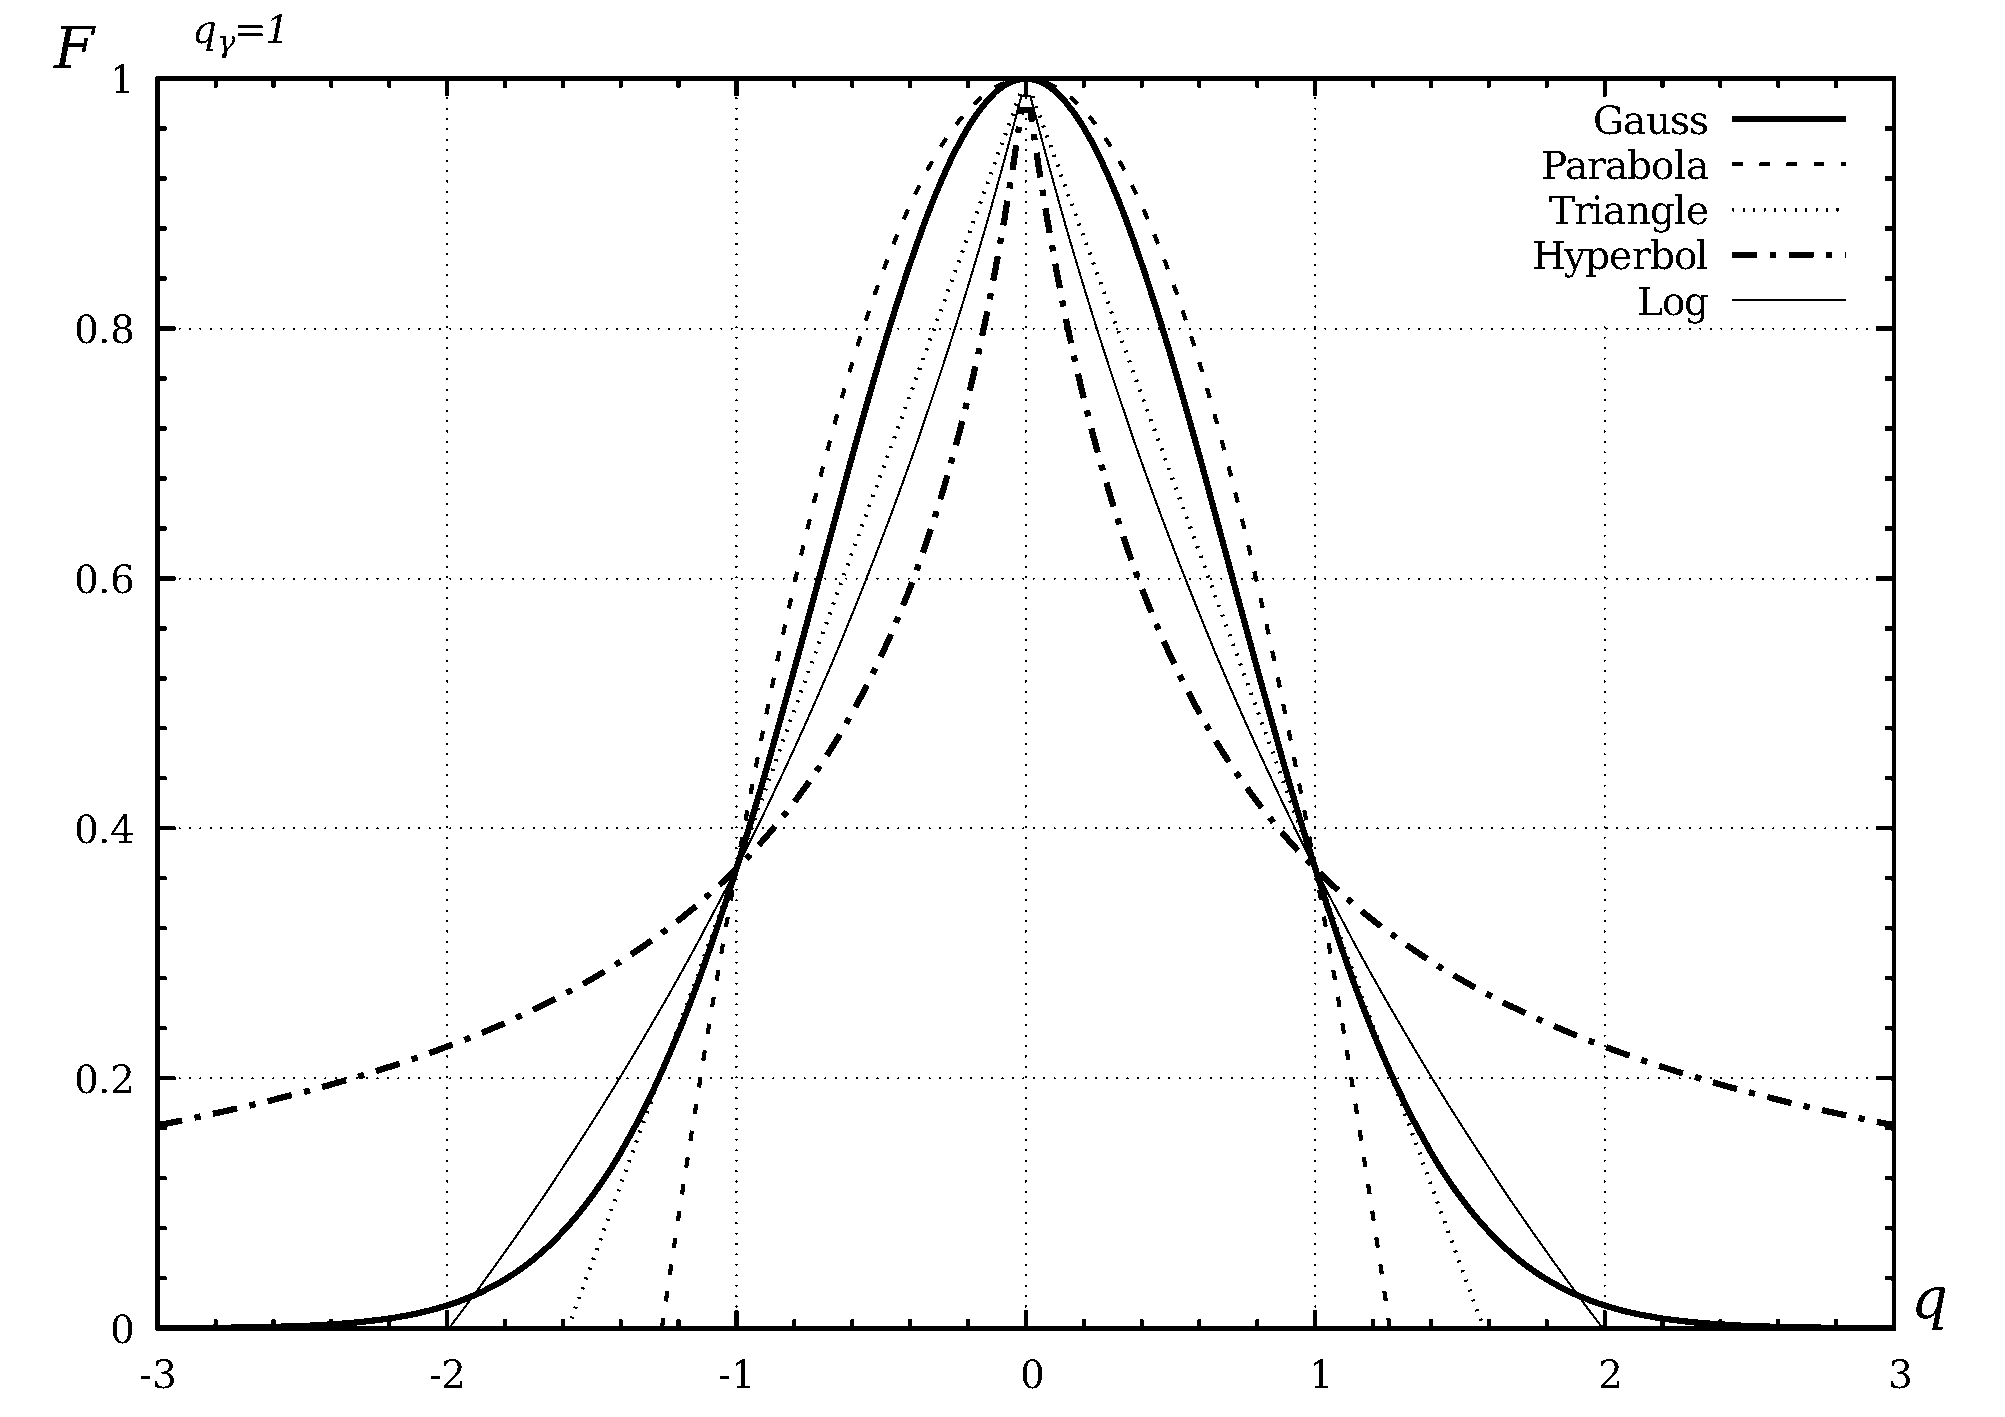
\includegraphics[width=55\TW]{p/F_types.png}
  \end{center}
  \caption{Функції якості ідентифікації (\ref{atu:eq:F_gauss})--(\ref{atu:eq:F_log})}
  \label{atu:f:F_types}
\end{figure}


% }}}2

% }}}1

\section{Структура пошукових систем} % {{{1


Введемо необхідні для подальшого викладу визначення.

Визначення:
\textbf{пошуковий агент} --- це динамічна система, яка отримує вихідні ($x(t)$),
і, при необхідності, вхідні ($u(t)$) сигнали від однієї або кількох моделей,
величину оцінки стану об'єкта за критерієм ідентифікації,
може обмінюватися інформацією з іншими елементами пошукової системи,
та, на підставі значення критерію
ідентифікації, реалізує алгоритм настройки параметрів моделі (моделей) таким
чином, щоб забезпечити визначення заданого параметра.

Визначення:
\textbf{координатор пошуку} --- це динамічна система, яка отримує інформацію
від пошукових агентів і на підставі цієї інформації визначає
$p_{\mathrm{id}}(t)$ --- величину ідентифікованого параметра.
Крім цього, координатор може, на підставі цієї ж інформації,
керувати процесом адаптації всієї пошукової системи.


Таким чином, система ідентифікації складається з множини агентів, та
множини координаторів пошуку, які спільно вирішують задачу ідентифікації.
За винятком ієрархічних систем ідентифікації, найчастіше використовується один координатор пошуку.

У найпростішому випадку, коли використовується один пошуковий агент, обов'язки
агента і координатора можуть бути поєднані. Якщо відкинути цей вироджений
випадок, найбільш простою є ``плоска'' структура системи ідентифікації (рис.~\ref{atu:f:agents_flat}).
При цьому координатор отримує
інформацію від усіх пошукових агентів, і, при необхідності, управляє ними.


\begin{figure}[htb!]
\begin{center}
../../p3/p/agents.pgf
\end{center}
\label{atu:f:agents_flat}
\caption{Мультиагентна система ідентифікації з плоскою структурою}
\end{figure}

У більш складних випадках може використовуватися ієрархічна
структура, при цьому кожен елемент, за винятком першого і
останнього рівня, служить як джерелом інформації для подальшого
рівня, так і координатором для попереднього. При цьому елемент
може як мати безпосередньо керовану модель, тобто виконувати
роль агента, так і задовольнятися роллю проміжного координатора.

Деякі конфігурації агентів і координаторів в даний час практично
застосовуються, можливо під іншими позначеннями і для інших задач, деякі
введені вперше. Розглянемо деякі конфігурації.

\textbf{Рій} --- множина агентів, що забезпечує ідентифікацію за рахунок
концентрації максимальної кількості агентів в області передбачуваного максимуму
функції якості або ж заданого значення критерію. Три складові поведінки: рух
до оцінюваного локального екстремуму, до глобального, випадкова складова.


Перевагою даного підходу є простота алгоритмів, які повинні
бути реалізовані агентами. Недоліки --- потрібно надмірна
кількість агентів. Значна частина агентів, що знаходяться
поблизу екстремуму, практично не приносить інформації. Ройовий
алгоритми (як і їх прообрази в живій природі) орієнтовані
для збільшення видобутку ресурсів, а не інформації. Також
недоліком можна вважати необхідність отримання інформації
від координатора (а саме, значення
$ p_\mathrm{id} $) кожним агентом для можливості визначення його
динаміки.

\textbf{Стрій} --- множина агентів, розташування яких, і якщо необхідно,
зміщення, задається однаковим чином. Відсутня індивідуальна динаміка кожного
агента. Нерухомий стрій утворює \textbf{сітку},
як рівномірно розподілену по простору параметрів, так і~ні.

Складність алгоритмів, що реалізується кожним агентом в цьому
випадку, простіше, ніж у випадку рою. Більш того, передача
інформації від координатора (в даному випадку ``командира'')
до агента є необов'язковою. Проте, можливості як адаптації, так
і просто підвищення точності ідентифікації у даного підходу
сильно обмежені.

\textbf {Ансамбль} ---
множина агентів, що забезпечує ідентифікацію за рахунок розподілу агентів таким
чином, який забезпечує як точність ідентифікації за рахунок обмеженого
скупчення агентів в областях передбачуваних максимумів функції якості, так і оперативного
переключення на інші області при зміні параметрів за рахунок недопущення
невиправданої скупченості агентів~\cite{atu_ric2016}.

Можливе застосування систем ідентифікації з структурами
і поведінкою вищого рівня, але в даній роботі вони не
розглядаються.

У цієї роботі основна увага приділяється саме пошуковим структурам типу
``ансамбль''. Очевидним недоліком даного підходу є відносна складність
алгоритмів, що реалізується пошуковими агентами.


% }}}1

\section{Властивості, параметри і алгоритми роботи пошукових агентів} %{{{1 -----------

\subsection{Задачі, вхідні і вихідні сигнали пошукових агентів} % {{{2

У відповідності до свого визначення, один пошуковий агент може керувати як
однією моделлю (рис.~\ref{atu:f:agent1}, \ref{atu:f:agent1q}),
так і кількома (рис.~\ref{atu:f:agent2}). При цьому він
може використовувати інформацію, як отриману безпосередньо від інших агентів,
так і обчислену в результаті обробки даних на інших рівнях системи
ідентифікації.

\begin{figure}[htb!]
\begin{center}
% vi:syntax=tex
\begin{tikzpicture}
  \bXStyleBloc{semiboldline,inner sep=2pt};
  \bXLineStyle{medline};
  % --- U
  \bXInput{U};
  % --- M
  \bXBlocL[2.0]{M}{$\mathbf{M}_i$}{U};
  \bXLink[$u(t)$]{U}{M};
  % --- Q
  \bXBloc[3.5]{Q}{$q(t)$}{M};
  \path (Q.east) ++(0.0,-1.0em) coordinate (Qqm);
  \path (Q.south west) ++(-0.3,-0.4) coordinate (BLKlb);
  \bXLink[$x_i(t)$]{M}{Q};
  % --- F
  \bXBloc[2.5]{F}{$F(q_o,q_{mi})$}{Q};
  \path (F.west) ++(0.0,-1.0em) coordinate (Fqm);
  \path (F.west) ++(0.0,+1.0em) coordinate (Fqo);
  \path (Fqo) ++(-1.6em,+2.8em) coordinate (Fqoi) {};  % external input
  \draw[medlinep] (Fqoi) |- (Fqo);
  \node[below right] at (Fqoi) {$q_o(t)$};
  \bXLink[$q_i(t)$]{Qqm}{Fqm};
  % --- P
  \bXBloc[2]{P}{$P$}{F};
  \draw[boldline,<->] (P.north) -- +(0,0.8);
  \path (P.north east) ++(0.1,+0.4) node (BLKrt) {};
  \bXLink[$F_i(t)$]{F}{P};
  % -- output
  \bXOutput[2.8]{Po}{P};
  \bXLink[$p_i(t)$]{P}{Po};
  \bXOutput[1.0]{Por}{P};
  \fill(Por) circle[radius=0.05];
  \bXLineStyle{semiboldline};
  \bXReturn{Por}{M}{$p_i(t)$};
  % -- block
  \draw[subelem] (BLKlb) |- (BLKrt) |- (BLKlb);
  \bXStyleBlocDefault;
  \bXDefaultLineStyle;
  %
  \TikzAddPadding
  %
\end{tikzpicture}

\end{center}
\caption{Пошуковий агент, який використовую функцію якості $F$, та управляє параметром однієї моделі}
\label{atu:f:agent1}
\end{figure}


\begin{figure}[htb!]
\begin{center}
% vi:syntax=tex
\begin{tikzpicture}
  \bXStyleBloc{semiboldline,inner sep=2pt};
  \bXLineStyle{medline};
  % --- U
  \bXInput{U};
  % --- M
  \bXBlocL[2.0]{M}{$\mathbf{M}_i$}{U};
  \bXLink[$u(t)$]{U}{M};
  % --- Q
  \bXBloc[3.5]{Q}{$q$}{M};
  \path (Q.east) ++(0.0,-1.0em) coordinate (Qqm);
  \path (Q.south west) ++(-0.3,-0.4) coordinate (BLKlb);
  \bXLink[$x_i(t)$]{M}{Q};
  % --- P
  \bXBloc[2]{P}{$P$}{Q};
  \draw[infoline,<->] (P.north) -- +(0,0.8);
  \path (P.west) ++(0.0,-1.0em) coordinate (Pqm);
  \path (P.west) ++(0.0,+1.0em) coordinate (Pqo);
  \path (Pqo) ++(-1.6em,+2.8em) coordinate (Pqoi) {};  % external input
  \path (P.north east) ++(0.1,+0.4) node (BLKrt) {};
  \bXLink[$q_{i}(t)$]{Qqm}{Pqm};
  \draw[medlinep] (Pqoi) |- (Pqo);
  \node[below right] at (Pqoi) {$q_o(t) \qquad A_i$};
  %\bXLink[$F_i(t)$]{F}{P};
  % -- output
  \bXOutput[2.8]{Po}{P};
  \bXLink[$p_i(t)$]{P}{Po};
  \bXOutput[1.0]{Por}{P};
  \fill(Por) circle[radius=0.05];
  \bXLineStyle{semiboldline};
  \bXReturn{Por}{M}{$p_i(t)$};
  % -- block
  \draw[subelem] (BLKlb) |- (BLKrt) |- (BLKlb);
  \bXStyleBlocDefault;
  \bXDefaultLineStyle;
  %
  \TikzAddPadding
  %
\end{tikzpicture}

\end{center}
\caption{Пошуковий агент, який використовую критерій $q$, та управляє параметром однієї моделі}
\label{atu:f:agent1q}
\end{figure}


\begin{figure}[htb!]
\begin{center}
% vi:syntax=tex
\begin{tikzpicture}
  %\draw[hair,step=1.0em] (0,-3) grid (12.0,3.0);
  \bXStyleBloc{semiboldline,inner sep=2pt};
  \bXLineStyle{medline};
  % --- U
  \bXInput{U};
  \path (U.center) ++(2.5em,0.0em) coordinate (UxM);
  \draw (U.center) -- (UxM);
  \fill (UxM) circle[radius=0.05];
  \node[above right] at(U) {$u(t)$};
  % --- M0
  \bXBranchy[2]{UxM}{U0};
  %\fill[red](U0) circle[radius=0.05];
  \bXBlocL[2.0]{M0}{$\mathbf{M}_{i0}$}{U0};
  \bXLinkyx{UxM}{M0};
  % --- M1
  \bXBranchy[-2]{UxM}{U1};
  %\fill[green](U1) circle[radius=0.05];
  \bXBlocL[2.0]{M1}{$\mathbf{M}_{i1}$}{U1};
  \bXLinkyx{UxM}{M1};
  % --- A
  \path (M0.east) ++(3.1em,0.0em) coordinate (X0);
  \path (X0) ++(4.0em,0.0em) coordinate (P0S);
  \path (X0) ++(0.0em,-2.0em) coordinate (Alb);
  %\fill[red](Alb) circle[radius=0.05];
  \path (M1.east) ++(3.1em,0.0em) coordinate (X1);
  \path (X1) ++(4.0em,0.0em) coordinate (P1S);
  \path (X1) ++(0.0em,2.0em) coordinate (Alt);
  \path ( $0.5*(P0S) + 0.5*(P1S)$ ) coordinate(PS);
  \path ( $0.5*(X0) + 0.5*(X1)$ ) coordinate(QO);
  \draw[medlinep] (QO) ++(-3.2em,0em) -- (QO);
  \node[above left] at(QO) {$q_{o}(t)$};
  %\fill[green](Alt) circle[radius=0.05];
  \draw[boldline] (Alb) -- ++(4.0em,0.0em) |- (Alt) -- cycle; % ----- MAIN block
  \draw[medlinep] (M0.east) -- (X0); // % inputs: x_ix(t)
  \node[above right] at(M0.east) {$x_{i0}(t)$};
  \draw[medlinep] (M1.east) -- (X1);
  \node[above right] at(M1.east) {$x_{i1}(t)$};
  \draw[semiboldlinep] (P0S) -- ++(3.0em,0em) -- ++(0em,-3.0em) -| (M0.south); % -- out params
  \node[above right] at(P0S) {$p_{i0}(t)$};
  \draw[semiboldlinep] (P1S) -- ++(3.0em,0em) -- ++(0em,+3.0em) -| (M1.north);
  \node[above right] at(P1S) {$p_{i1}(t)$};
  \draw[medlinep] (PS) -- ++(4.0em,0em);
  \node[above right] at(PS) {$p_{i}(t)$};
  \path (PS) ++(-2.1em,0.0em) coordinate (AI);
  \node at(AI) {$\mathbf{A}_{i}$};
  %
  \TikzAddPadding
  %
\end{tikzpicture}

\end{center}
\caption{Пошуковий агент, який управляє параметрами двох моделей}
\label{atu:f:agent2}
\end{figure}

Для спрощення позначень величин, що належать різним агентам, ведемо
позначення. Якщо в даному контексті важливо вказувати індекс агента, то він
вказується явно, наприклад: $F_{c, i} (t)$ --- значення функції якості для
центральної (``c'') моделі агента з індексом ``i''. У тих випадках, коли
обрано конкретний агент або коли позначення застосовується до всієї множині
агентів, індекс можна вилучити, наприклад: $ p_e (t)$
--- оцінка значення параметра для поточного агента або ж для агентів взагалі.
Для позначення найближчого околу агента використовуємо такі позначення:
``c'' --- ``center'' --- позначає центральну або єдину модель агента або ж
відноситься до агенту в цілому, ``l'' --- ``left'' --- позначає, в
залежності від контексту, або величину, яка відноситься до попереднього (за
індексом) агенту, або ж першу модель (з двох або трьох), яка використовується
агентом, ``r'' --- ``right'' --- аналогічно, але в протилежну сторону у
просторі індексів.
Якщо ж необхідно вказати індекс агента, а величина щодо
об'єкта має позначення ``c'', то цю частину позначення можна опустити,
наприклад: $p_i (t) \equiv p_{i, c} (t)$, $q_{i , c} \equiv q_{i} (t)$.
Всі індекси одночасно опускати не можна, однак, в очевидних випадках можна
опускати явну залежність від часу: $q_l (t) \equiv q_l$. При необхідності,
що величина відноситься до моделі, без вказівки конкретного індексу моделі,
будемо використовувати індекс ``m'', наприклад $x_m$ --- вихідний сигнал
заданої (або ж єдиною) моделі.

У разі, коли один агент налаштовує кілька моделей, або, якщо
простір параметрів має розмірність більше одиниці, замість
простого індексу
$ i $ можуть застосовується складові.

Кожен агент на підставі як власних вимірів, так і інформації, отриманої від
інших агентів, оцінює значення $p_e (t)$, яке, за його даними, найближче до
параметра об'єкту $p_o(t)$.
Частина методів використовує це подання неявним чином. При цьому,
якщо значення $p_e$ виходить за межі значень параметрів моделей, на підставі
яких було отримано це значення, то його слід вважати сумнівним.
Ступінь ``впевненості'' в розрахунковому значенні $p_e$ позначимо $S \in [0; 1] $\label{atu:d:S} (surety).
В результаті такі оцінки в подальшому можна як
взагалі не враховувати при розгляді, так і обмежити їх вплив на наступному
рівні.
Або --- можна обмежити область допустимих значень $p_e$
значеннями параметрів моделей, що використовуються.

Вихідними сигналами агента є:\label{atu:d:agent_out_list}

\begin{itemize}

  \item
    $p_c(t)$ ---
    поточне значення параметра.

  \item
    $p_e(t)$\label{atu:d:p_e} --
    поточне значення оцінки параметра.

  \item
    $F_c(t)$ ---
    поточне значення функції якості (якщо використовується одна
    модель для агента, або ж якщо агент якимось чином її усередняє
    або апроксимує в разі декількох моделей). Може поєднувати
    функції вхідного і вихідного сигналів.

  \item
    $q_c(t)$ ---
    значення критерію якості (аналогічно попередньої величиною в
    разі декількох моделей); спочатку цей сигнал був представлений
    як вхідний для агента, проте він може використовуватися і
    на більш високих рівнях системи ідентифікації. Якщо ж агенту
    значення критерію недоступно, то і в списку вихідних сигналів
    ця величина також відсутня.

  \item
    $F_e(t)$ ---
    апроксимоване значення функції якості в точці
    $p_e(t)$. Якщо агент не використовує для роботи апроксимацію
    $ F $, то і відповідний вихідного сигнал не використовується.

  \item
    $S(t)$ ---
    ступінь ``впевненості'' агента в отриманому значенні.

\end{itemize}

Деякі з цих сигналів можуть не використовуватися в конкретної
реалізації координатора пошуку. Наприклад, системи
ідентифікації з одним агентом практично не потребують величини
$S(t)$. Величина
$q_c(t) $ досить рідко використовується при роботі
координатора. Досить часто використовуються похідні сигнали,
наприклад
$ W(t) = F_c(t) S(t) $\label{atu:d:W} (worthiness), який поєднує як локальну впевненість
агента в оцінці
$ p_\mathrm{id} (t) $, так і глобальну функцію якості. Також зазначені
сигнали можуть використовуватися самим агентом безпосередньо,
для визначення власної динаміки.


Агенти, для оцінювання величини $p_e$ можуть використовувати як значення
критеріїв ідентифікації $q$ безпосередньо, так і тільки значення функцій
якості, які відповідають критеріям.

Принципової різниці між конфігураціями ``один агент --- пара моделей''
і ``два агента, кожен управляє однією моделлю''
немає. Для визначеності будемо вважати, що якщо підтримується
постійна різниця між значеннями параметрів моделей, або ж ця
різниця визначається одноманітно, то це --- один агент. Якщо ж
різниця не визначається безпосередньо, і є наслідком динаміки
кожної моделі, то має сенс говорити про пару агентів.

Проте, при використанні пари моделей невиправдано багато часу
витрачається на переміщення пошукової пари, особливо при різких
змінах ідентифікованого параметра~\cite{atu_asau23}.
Тому, використання множини
пошукових агентів може кардинально зменшити час ідентифікації.


Розглянемо випадок, коли кожен агент
керує двома моделями.

Для систем ідентифікації, що використовують тільки один
агент з двома моделями, це досить непоганий варіант. Якщо ж
використовувати кілька агентів, кожен з парою моделей,
то моделі в цій системі будуть використовуватися
нераціонально. Розглянемо випадок, коли значення параметрів
моделей розподілені в просторі параметрів послідовно, і
значення параметра, відповідне
$ q_o $ лежить між значеннями параметрів пари сусідніх моделей. При
цьому, якщо пара моделей належить одному агенту, то він, а отже,
і вся система ідентифікації може досить точно оцінити значення
$ q_o $.
Якщо ж моделі цієї пари належать різним агентам ---
то задача оцінки вирішується вже координатором,
що, може привести до росту похибки ідентифікації.

Для того, що б нівелювати цей недолік, створимо структуру системи
ідентифікації, в якій кількість моделей дорівнює кількості
агентів, не рахуючи, може бути, додаткових моделей на границі
робочої області.
Кожен агент безпосередньо управляє однією моделлю,
та отримує інформацію від двох найближчих агентів
про значення параметра і критерію ідентифікації
(або функції якості) їх моделей~(рис.~\ref{atu:f:agents_flat}).
При цьому кожна модель має вплив на трійку агентів,
і навпаки, кожен агент отримує інформацію від трьох моделей.
Кожна модель входить у три трійки, та ці трійки обробляються за
однаковими правилами.


Обробка границь робочої області потребує додаткових підходів.
Для того, що б обробити границю
пошукової області є кілька підходів, які потребують визначення
додаткових моделей, використання яких і забезпечує як обмеження
області пошуку, так і єдинообразності алгоритмів для агентів
всередині. Надалі будемо позначати їх індексами ``ll'' і~``rr''.

Перший з підходів реалізується найбільш простим способом і
практично не вимагає витрат. В цьому випадку для однаковості
множина моделей доповнюється двома (в одновимірному випадку)
нерухомими псевдомоделямі (fake models). Для псевдомоделей вважаємо
$ F_{ll} = F_{rr} = 0 $, а координати вибираються за межами робочого
діапазону пошуку. Застосування цього підходу найбільш
виправдано для агентів, що обчислюють значення
$p_e$ на підставі значень функції якості. При цьому, платою за менші обчислювальні
витрати є поява  впливу ``стису'' на весь ансамбль у
цілому. Системи з агентами, які використовують для визначення
$p_e$ безпосередньо значення критерію, не можуть безпосередньо
скористатися цьому підходом, так як нульового (або близькому
до нульового) значення функції якості зазвичай відповідає
необмежена множина значень критерію.

Другий підхід відрізняється застосуванням нерухомих
справжніх моделей на границі робочої області. При цьому,
агенти, що є сусідами цих моделей, можуть використовувати
значення як параметрів, так і критеріїв цих моделей природним
чином. Основним недоліком цього підходу є додаткова витрата
ресурсів для моделей на границі. Також застосування таких
моделей може бути не виправданим у  тих випадках, коли моделювання за межами
(або безпосередньо на границі) неможливо через порушення
стійкості моделей. Тим не менш, цей підхід, з одного боку,
дозволяє коректно застосовувати агентів, які використовують
$q$ для визначення $p_e$,
а з іншого --- дозволяє позбутися від впливу, що ``стискає'' при
використанні агентів, які використовують~$F$.

Проміжним варіантом є підхід, при використанні якого
теж використовуються псевдомоделі, але замість нульового
значення функції якості використовується або яким-небудь чином
апроксимоване значення
$ F $, (може бути застосовано і до $q$),
або отримане в результаті попереднього моделювання.

% }}}2



\subsection{Методи визначення шуканого значення параметра одним агентом} % {{{2

Першою із задач, що постають перед агентом ідентифікації, є визначення $p_e(t)$
на підставі наявних даних, а також оцінка впевненості $S(t)$ в
отриманому значенні.

Системи пошукової та адаптивно-пошукової ідентифікації,
які використовуються для роботи з звичайними нелінійними
динамічними системами, в якості вихідних даних як для визначення
безпосередньо шуканого параметра, так і для побудови пошукової
траєкторії використовували безпосередньо вихідні сигнали
об'єкта ($x_o(t)$) і моделі~($x_m(t)$).
При цьому явно або неявно використовувалася функція
якості. Більш того, при певних умовах, з урахуванням інерційних
та усереднювати властивостей системи ідентифікації такий
підхід, неявним чином, використовував один з енергетичних
критеріїв.

При ідентифікації систем хаотичної динаміки використання
критерію ідентифікації є обов'язковим. Природно, це може
бути застосовано і для систем, що не проявляють хаотичну
динаміку. При цьому агент, для виконання своїх задач, може
використовувати як саме значення критерію, так і відповідне
йому значення функції якості. Алгоритми, що використовуються
агентами в цих випадках, будуть істотно відрізнятися. В першу
чергу це пов'язано з тим, що парний вид функцій якості спонукає
використовувати для визначення максимуму методи, характерні
для систем екстремального керування~\cite{rastr_seu}.

Для несуперечності і збереження працездатності системи
ідентифікації в широких межах має сенс розглянути набір
необов'язкових, але бажаних вимог:

\begin{itemize}

  \item
    В першу чергу, при лінійної залежності
    $q(p)$ і відсутності помилок вимірювання похибка оцінювання
    ``своєї'' точки
    $p_e$ повинна бути досить малою. Порушення цієї вимоги
    ускладнює роботу системи ідентифікації при наближенні до
    ідентифікованому значенню.

  \item
    По-друге, при цих же умовах глобальні оцінки
    $ p_o $ також повинні також характеризуватися досить малими
    похибками, в іншому випадку втрачається сенс використання
    декількох агентів.

  \item
    Зближення і віддалення пошукових агентів в межах призначених
    діапазонів не повинно приводити до істотної зміни величини
    ідентифікованого значення. Ця вимога здебільшого здійснима
    тільки на досить ``хороших'' видах критеріїв, без переважаючого
    впливу високочастотних нелінійних ефектів, проте сам метод не
    повинен вносити істотні додаткові спотворення на даному етапі.

\end{itemize}

Слід також зазначити, що для реальних задач
$ q_o (p) \ne q_m (p) $, зважаючи як обмеженості моделей, так і перешкод
виміру. Проте, в цьому розділі даний факт буде ігноруватися
з метою вивчення можливостей і помилок власне методів
ідентифікації.




Як вже було зазначено, в вписок задач агента входить не тільки
визначення величини
$ p_e $, але і оцінка власної ``впевненості''
$ S $ в отриманому значенні. Розглянемо фактори, які може враховувати
агент при вирішенні цієї задачі.

\begin{enumerate}

  \item
    Відносна віддаленість точки
    $ p_e $ від точок, що використовувалися при її визначенні. При
    цьому може братися до уваги або тільки центральна точка
    $ p_c $, або ж враховуватися точки сусідніх агентів.

  \item
    Розташування
    $ p_e $ щодо використовуваних агентів. Як правило, похибки при
    інтерполяції помітно менше помилок при екстраполяції,
    і це необхідно враховувати. Також, сама конфігурація
    використовуваних точок може бути більш або менш сприятлива для
    оцінки~$p_e$.

  \item
    При використанні деяких методів є можливість оцінити
    нелінійність залежності
    $q(p)$, і отже, врахувати це при визначенні
    $ S $, за допомогою коефіцієнта~$k_l$.

  \item
    При оцінці можуть виникати особливі випадки, що перешкоджають
    нормальній роботі методу. Отже, такі випадки вимагають
    застосування особливих правил при обчисленні~$S$.

\end{enumerate}

Пропонуються наступні
методи визначення $S$ при отриманні агентом інформації з трьох моделей:
%
\begin{equation}
  S_1 = c_\mathrm{su} \exp \left( - \frac{ \big( k_l c_\mathrm{dist} ( p_e - p_c ) \big)^2 }{p_b^2} \right)
  ,
  \label{atu:eq:S1}
\end{equation}
%
\begin{equation}
  S_3 = c_\mathrm{su} \exp \left( - \frac{ \big( k_l c_\mathrm{dist} \min( |p_e - p_l|,|p_e - p_c|, |p_e - p_r| ) \big)^2 }{p_b^2} \right)
  .
  \label{atu:eq:S3}
\end{equation}
%
де
$c_\mathrm{su}$ ---
коефіцієнт, що відображає працездатність методу в даному випадку;
$c_\mathrm{dist}$ ---
коефіцієнт, що визначає ``штраф'' або ``бонус'', пов'язаний з відносним розташуванням робочих точок;
$k_l$ ---
коефіцієнт оцінки нелінійності системи;
$p_b$ ---
характерний масштаб, щодо якого враховується видалення $p_e$ від використаних точок.


У випадках, коли агенти рівноправні, має сенс використовувати визначення
(\ref{atu:eq:S3}), так як похибка визначення $p_e$ в першу чергу визначається її
віддаленістю від найближчого агента. В даній роботі, якщо не вказано інше, буде
використовуватися саме це визначення.
Використовувати визначення (\ref{atu:eq:S1}) має сенс в тих випадках,
коли інформація, отримана від сусідніх агентів, менш надійна,
ніж від поточного, наприклад, при використанні псевдомоделей.

\paragraph{Демонстраційна задача}

Для демонстрації способів визначення пошуковим агентом величини $p_e$ в
стаціонарному або квазістаціонарному випадку введемо наступну штучну залежність~$q(p)$:
%
\begin{equation}
  q_\mathrm{dem}(p) = q_{00} + c_\mathrm{lin} \tilde{p} + c_\mathrm{s1} \sin( \pi \tilde{p} ) + c_\mathrm{s2} \sin( 2 \pi \tilde{p} ) + c_\mathrm{s20} \sin( 20 \pi \tilde{p} ),
  \label{atu:eq:q_dem}
\end{equation}
%
де
$q_{00}$, $c_\mathrm{lin}$, $c_\mathrm{s1}$, $c_\mathrm{s2}$, $c_\mathrm{s20}$
--- коефіцієнти, що дозволяють налаштувати цю залежність для перевірки заданого аспекту поведінки агента,
$ \tilde{p} = \frac{p - p_{\min}}{p_{\max} - p_{\min}} $ ---
параметр, приведений до безрозмірного вигляду.
При цьому
$\tilde{p} \in[0;1]$, $c_\mathrm{lin} \ne 0$
визначає лінійну частину залежності,
$c_\mathrm{s1}$ і $c_\mathrm{s2}$
визначають нелінійну частину, що має характерний масштаб порядку робочого діапазону $p$,
$c_\mathrm{s20}$
визначає високочастотну складову цієї залежності.
Якщо $c_\mathrm{s1} = 0$, $c_\mathrm{s2}=0$, $c_\mathrm{s20}=0$,
то задача визначення $p_e$ є тривіальною,
але такий випадок також є корисним при аналізі поведінки агента.

Надалі будемо використовувати ці позначення при описі різних
режимів роботи методів ідентифікації, а також при моделюванні
тестових завдань.

Розглянемо можливі способи визначення
$ p_e $ для агентів, які використовують як критерій ідентифікації
безпосередньо, так і функції якості.

% }}}2


\subsection{Методи агентів, які використовують значення критерію} % {{{2

Нерухомий агент, який використовує для своєї роботи тільки одну модель, і,
відповідно, характерне для неї значення критерію, практично не має самостійного
сенсу.
Реальна користь від такого агента може бути тільки в тому
випадку, коли координатор якимось чином зміг оцінити залежність
$q(p) $ цілком, і передав або цю залежність агенту, або за його
запитом обчислює
$p(q)$. Очевидно, що в такому випадку ніякі пошукові агенти не
потрібні, і можна просто обчислити~$p (q_o)$.

Якщо агент, який використовує одну модель є рухомим, то він може
оцінити своє становище, використовуючи історію. Подання історії
може мати різні форми. Наприклад, агент може зберігати значення
$ p_c $,
$ q_c $ для моменту часу в минулому, віддаленому від поточного часу
на задане значення. Може бути застосований будь-який
фільтр, в якому вплив різних моментів минулого враховується з
різними коефіцієнтами. Також в якості опції уявлення історії
може використовуватися динаміка самого ідентифікованого
об'єкта~\cite{mich_92}.

Розглянемо випадок, коли один рухливий агент і отримує дані з
двох моделей,
$ \mathbf{M}_{il}$ и
$ \mathbf{M}_{ir}$,
і керує ними однаковим чином, наприклад витримуючи постійну
відстань
$ \Delta p $ між ними в просторі параметрів. У цьому випадку він може
оцінити, яка з моделей ближче за критерієм до об'єкта, і оцінити стан
$ p_o $ як $ p_e $.

Розглянемо групу з трьох агентів:
$\mathrm{A}_l$,
$\mathrm{A}_c$,
$\mathrm{A}_r$.
Агент $\mathrm {A} _c$ зі значенням параметра $p_c$ сам визначає величину
$q_c$, від сусідніх агентів отримує значення $p_l$, $q_l$, $p_r$, $q_r$.
Будемо вважати, що динаміка агентів визначена так, що
$p_l(t) < p_c (t) < p_r(t) \; \forall t$.
Система ідентифікації забезпечує кожного агента
значенням $q_o$.
Зважаючи на все вищезазначене,
задача
визначення $p_e$ полягає в знаходженні такого $p$, яке відповідає перетину
невідомою кривої, заданої трьома точками, з прямою $q = q_o$.
Формально, з урахуванням введених обмежень, три точки однозначно визначають параболу. Однак,
застосування параболічної апроксимації в умовах високого рівня перешкод
найчастіше невиправдано~\cite{atu_asau27}.
Більш того, в цьому випадку буде потрібна додаткова
логіка як для вибору підходящого кореня, так і для визначення ``впевненості''
в отриманому рішенні.
Тому, будемо розглядати кусково-лінійне наближення з
аналізом отриманої конфігурації. Існує чотири можливих конфігурації,
кожна з яких потребує окремого рішення.

Розглянемо можливі конфігурації в порядку, що забезпечує
несуперечність алгоритму.

\paragraph{Випадок 1.}
Це особливий випадок, коли значення
$ p_c $ агента досить добре збігається з шуканим значенням. Поняття
``досить добре'' в даному випадку визначається постановкою
задачі ідентифікації, і може бути задано граничним значенням функції якості:
$ F_c> F_{\mathrm{good}} $, де
$ F_{\mathrm{good}} $ вибирається досить близько до одиниці. При цьому
вважаємо:
%
\[
p_e = p_c, \; c_\mathrm{su} = 1, \;  c_\mathrm{dist} = 1, \;  k_l = 1, \;  p_b = p_r - p_l,
\]
%
що дає
$ S = 1 $, тобто агент повністю ``впевнений'' в отриманому значенні
$ p_e $. Якщо є явне обмеження на використання функції якості
безпосередньо агентом, то слід задати допуск на значення
критерію:
$ |q_c-q_o| < q_{\min}$.

Практично, для кількох агентів може одночасно виконуватись
ця умова, і подальше визначення
$ p_\mathrm{id} $ в цьому суперечливому випадку покладається на
координатора пошуку. Якщо дана ситуація в процесі пошуку
трапляється досить рідко, то це, як правило, не порушує загальну
динаміку пошуку. Якщо ж цей випадок виявляється досить часто,
то це свідчить про грубі прорахунки при синтезі системи
ідентифікації. Наприклад, така поведінка може бути викликана
застосування критерію, невідповідного для даної задачі,
або ж занадто заниженим значенням чутливості функції якості.

Слід зазначити, що в цьому випадку у агента немає необхідності
аналізувати значення, отримані від сусідніх агентів. Це дозволяє
уникнути ряду ситуацій, в яких алгоритм пошуку буде давати
збої, які пов'язані з невизначеністю алгоритмів пошуку в вироджених
випадках.
%
В першу чергу, якщо
$F_c \le F_\mathrm{good}$, то $q_o -q_c \ne 0$,
і можна застосувати наступні перетворення:
%
\[
  \tilde{p}_l = p_l - p_c;
  \quad
  \tilde{p}_c = p_c - p_c = 0;
  \quad
  \tilde{p}_r = p_r - p_c;
  \quad
  \tilde{p}_e = p_e - p_c;
\]
%
\begin{equation}
  \tilde{q}_l = \frac{q_l-q_c}{q_c-q_o};
  \quad
  \tilde{q}_c = \frac{q_c-q_o}{q_c-q_o} = 1;
  \quad
  \tilde{q}_l = \frac{q_l-q_c}{q_c-q_o}.
  \label{atu:eq:q_agent_rel}
\end{equation}
%
При цьому критерій приводиться до безрозмірного вигляду,
причому точку відліку і одиничну довжину визначають величини
$q_c$ и $q_o$, так як $\tilde{q_c} = 1$ і $\tilde{q_o} = 0$.
У просторі параметрів відбувається тільки зміщення точки відліку.

Зважаючи на ці позначення, визначимо оцінку
$\tilde{p}_e$
для кожної з ділянок незалежно:
%
\begin{equation}
  \tilde{p}_{el} = \frac{\tilde{p}_l}{1-\tilde{q}_l},
  \quad
  \tilde{p}_{er} = \frac{\tilde{p}_r}{1-\tilde{q}_r}.
  \label{atu:eq:pr_ex}
\end{equation}

Випадок точної рівності нулю знаменника в цих виразах відповідає нескінченно
далекому розташуванню $p_e$, повної непевності в отриманому рішенні ($S = 0$)
і алгоритмічно виключається.


\paragraph{Випадок 2.} % brIdx = 3,4,5,6
%
Всі значення
$q_l $, $q_c $, $q_r $ знаходяться по одну сторону сторону від прямої
$q = q_o$, що еквівалентно умові
$\tilde{q}_l> 0 $ і $\tilde{q}_r> 0 $.
В цьому випадку слід прийняти, що
$p_e \notin [p_l, p_r] $, тобто за даними поточних трьох моделей немає
можливості досить впевнено визначити
$ p_e $. Проте, завдання оцінити
$ p_e $ все одно залишається актуальною. Якщо система ідентифікації
використовує тільки одного агента, то значення
$ p_e $, нехай навіть ненадійне, необхідно для визначення динаміки
агента, і відповідно, зміщення його в бік області, де оцінка буде
більш обґрунтованою. Якщо ж використовується мультиагентна
система, то отримане значення
$ p_e $ досить або обмежити штучно, або зменшити його значимість
за рахунок зниження величини
$ c_\mathrm{su} $.

При аналізі даного випадку необхідно розглянути кілька
варіантів.

Варіант A.\label{atu:d:p_eql_2A} % brIdx = 3
%
Центральна точка --- найкраща~(рис.~\ref{atu:f:pq_2A}),
т.е $\tilde{q}_l > 1 $ і $\tilde{q}_r > 1  $.

\begin{figure}[htb!]
  \begin{center}
    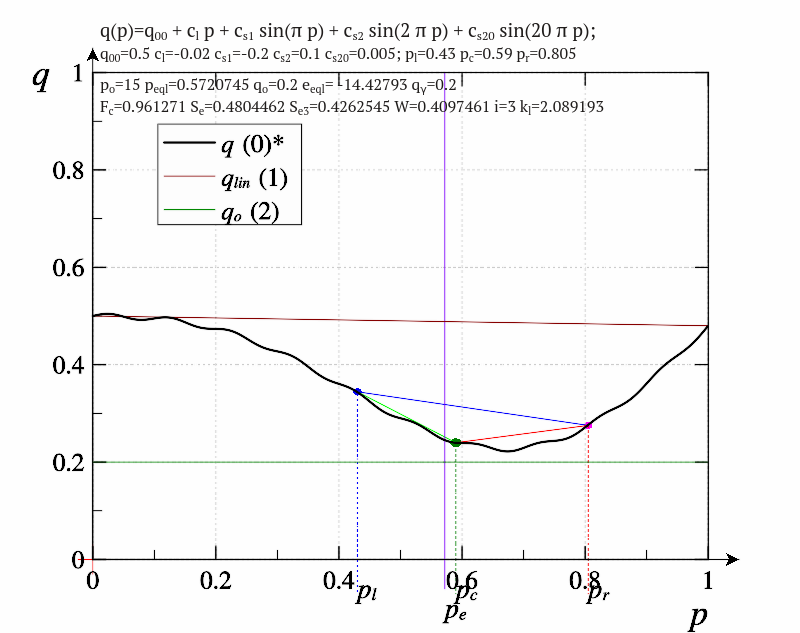
\includegraphics[width=60\TW]{p/pq_sin-p_pq_cgood.png}
  \end{center}
  \caption{Конфігурація точок, відповідна варіанту 2A}
  \label{atu:f:pq_2A}
\end{figure}

Як видно з графіка, це досить нетривіальна конфігурація, яка
може відповідати локальному наближенню
$ q (p) $ до
$ p_o $, що для гарного критерію нехарактерно, тимчасової
конфігурації робочих точок через вплив перешкод, а також
можливості реального знаходження
$ p_o $ в поточному робочому діапазоні, але через певні причини,
перш за все сильної нелінійності
$p(q)$ неправильної оцінки його положення. На підставі наявної
інформації складно зробити висновок про реальні причини, тому
в цьому випадку проводиться мінімальна коригування положення,
і впевненість в отриманому рішенні невелика:
%
\begin{equation}
  \tilde{p}_e = 0.1 ( \tilde{p}_{el} + \tilde{p}_{er} ),
  \;
  c_\mathrm{su} = 0.2, \;  c_\mathrm{dist} = 4, \;   p_b = p_r - p_l,
  \label{atu:eq:pr_e_2A}
\end{equation}



Варіант B.\label{atu:d:p_eql_2B} % brIdx = 4,5
%
Центральна точка --- проміжна~(рис.~\ref{atu:f:pq_2B}),
що відповідає умові
$ ( \tilde{q}_l -1 ) \cdot ( \tilde{q}_r -1 ) < 0 $.

\begin{figure}[htb!]
  \begin{center}
    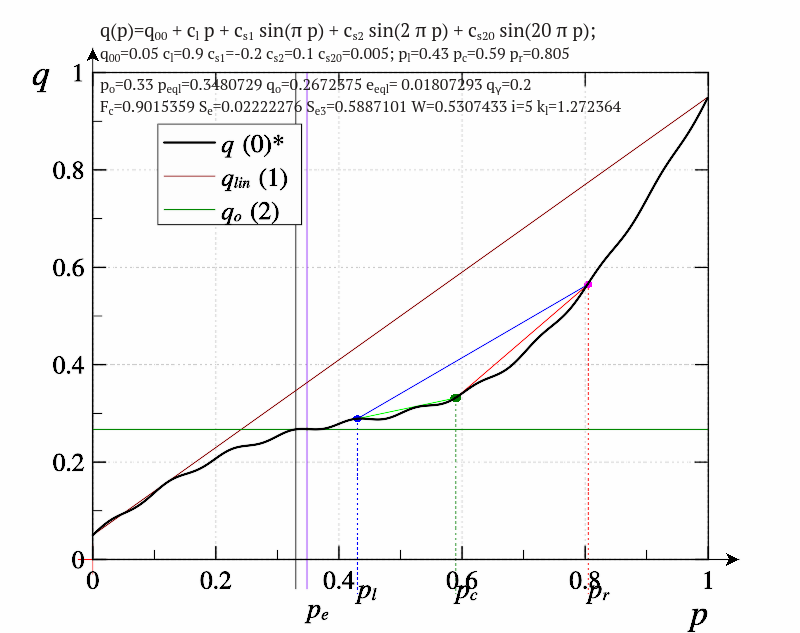
\includegraphics[width=49\TW]{p/pq_sin-p_pq_po=033.png}
    \hfill
    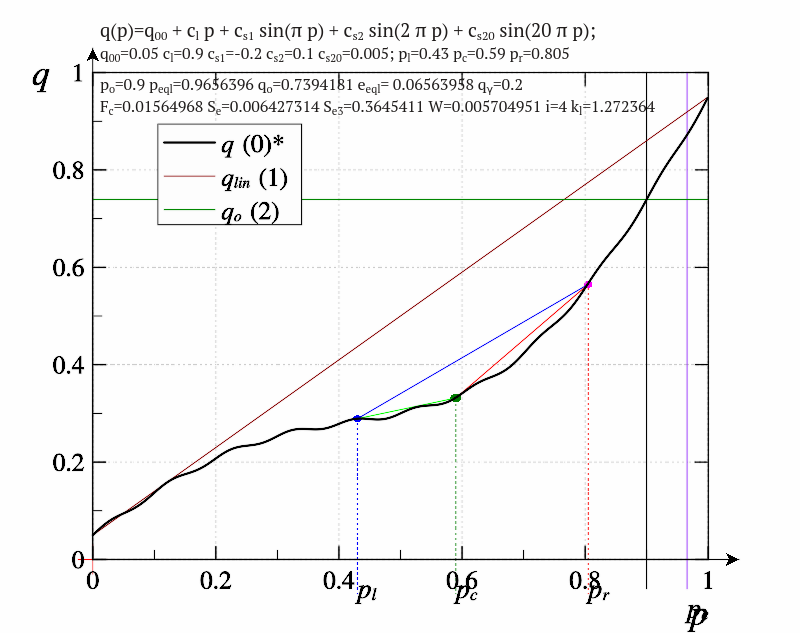
\includegraphics[width=49\TW]{p/pq_sin-p_pq_po=090.png}
  \end{center}
  \caption{Розміщення точок, відповідні випадку 2B}
  \label{atu:f:pq_2B}
\end{figure}

Ця конфігурація не є невизначеною, як в попередньому випадку,
і відповідає екстраполяції залежності за межі
$[p_l, p_r]$. У цьому випадку будемо використовувати
%
\begin{equation}
  \tilde{p}_e
  =
  \begin{cases}
    \tilde{p}_{el}, & \tilde{q}_l < \tilde{q}_r
    \\
    \tilde{p}_{er}, & \text{ otherwise}.
  \end{cases}
  ,
  c_\mathrm{su} = 0.9, \;  c_\mathrm{dist} = 2,  \;
  p_b =
  \begin{cases}
    -\tilde{p}_l, & \tilde{q}_l < \tilde{q}_r
    \\
    \tilde{p}_r, & \text{ otherwise}.
  \end{cases}.
  \label{atu:eq:pr_e2B}
\end{equation}

Щодо високе значення
$ c_\mathrm{su} $ і досить обмежене значення
$ c_\mathrm{dist} $ підкреслюють той факт, що незважаючи на наявність
екстраполяції, метод в цьому випадку може давати непогані
результати.


Варіант C. \label{atu:d:p_eql_2C}% brIdx = 6
%
Центральна точка --- найгірша~(рис.~\ref{atu:f:pq_2C}).

\begin{figure}[htb!]
  \begin{center}
    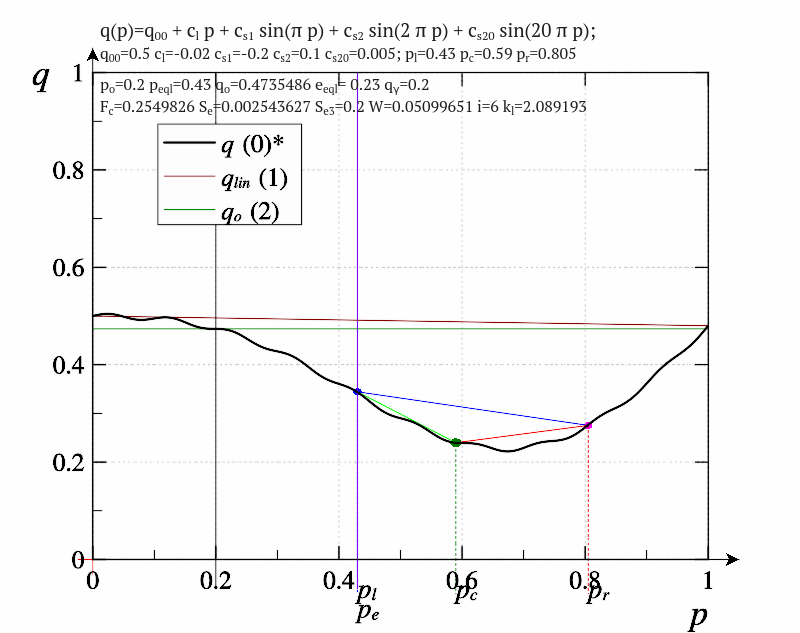
\includegraphics[width=60\TW]{p/pq_sin-p_pq_cbad.png}
  \end{center}
  \caption{Конфігурація точок, відповідна варіанту 2C}
  \label{atu:f:pq_2C}
\end{figure}

Цей варіант один з найменш сприятливих для визначення
$ p_e $, ще більш невизначений в порівнянні з випадком~2A. У цьому
випадку в якості
$ p_e $ можна взяти кращу з крайніх точок, при цьому нульова
відстань від цієї точки у визначенні
$ S $ необхідно компенсувати істотним штрафом в значенні
$ c_\mathrm{su} $, інші коефіцієнти при цьому значення не мають:
%
\begin{equation}
  \tilde{p}_e
  =
  \begin{cases}
    \tilde{p}_{l}, & \tilde{q}_l < \tilde{q}_r
    \\
    \tilde{p}_{r}, & \text{ otherwise}.
  \end{cases}
  ,
  c_\mathrm{su} = 0.1 .
  \label{atu:eq:pr_e2C}
\end{equation}

\paragraph{Випадок 3.}% brIdx = 10
%
Значення
$ q_l $ і
$ q_r $ розташовані по одну сторону від прямої
$ q = q_o $, а
$ q_c $ --- по іншу, тобто існують два кореня в даній
області~(рис.~\ref{atu:f:pq_3}).

\begin{figure}[htb!]
  \begin{center}
    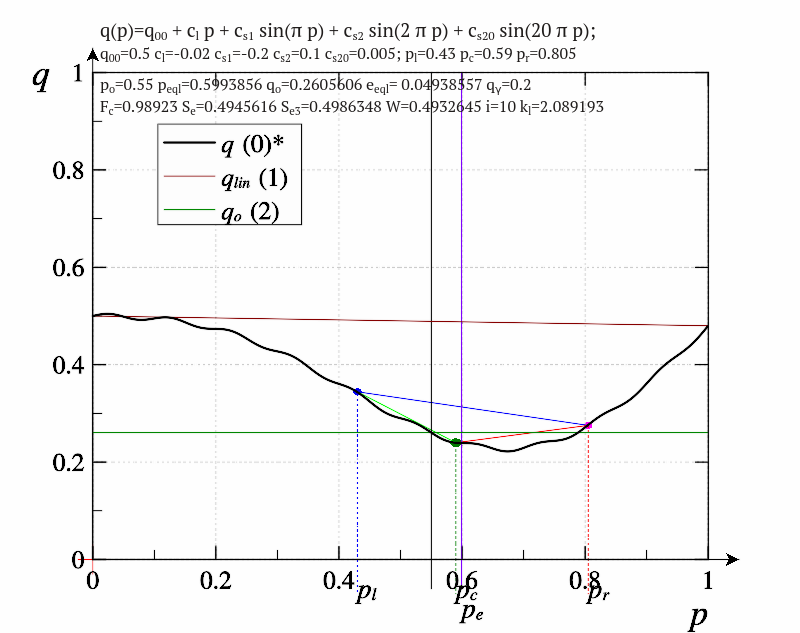
\includegraphics[width=60\TW]{p/pq_sin-p_pq_double.png}
  \end{center}
  \caption{Конфігурація точок, відповідні варіанту 3}
  \label{atu:f:pq_3}
\end{figure}

Це досить нетривіальний випадок, і при правильному критерії
та ідеальних умовах зустрічатися не повинен. Однак, в реальних
умовах, при наявності похибок вимірювання і недосконалості критерію
даний випадок цілком можливий (нехай і досить рідко), і вимагає
окремої обробки. Більш того, на відміну від невизначених
випадків 2A і 2C, даний свідчить про те, що питомі значення дійсно
лежить в поточному робочому діапазоні, але перешкоди і
нелінійності не дають можливості встановити його точне
положення. При цьому, якщо для визначення
$ p_e $ вибрати один з інтервалів
$ [p_l, p_c] $ і
$ [p_c, p_r] $, то цей вибір, з урахуванням перешкод, буде практично
випадковим, і малі зміни в значеннях критерію можуть перемкнути
на іншу гілку. Тому, для визначення
$ p_e $ використовуємо підхід, аналогічний застосований у випадку~2A,
але з іншими коефіцієнтами:
%
\begin{equation}
  \tilde{p}_e = 0.1 ( \tilde{p}_{el} + \tilde{p}_{er} ),
  \;
  c_\mathrm{su} = 0.5, \;  c_\mathrm{dist} = 2, \;   p_b = \frac{p_r - p_l}{2}.
  \label{atu:eq:pr_e_3}
\end{equation}


\paragraph{Випадок 4.}
%
Дві послідовні точки
розташовані по один бік
від прямої
$q = q_o$, а решта --- по інший, тобто в робочому діапазоні існує тільки один
корінь~(рис.~\ref{atu:f:pq_4}).


\begin{figure}[htb!]
  \begin{center}
    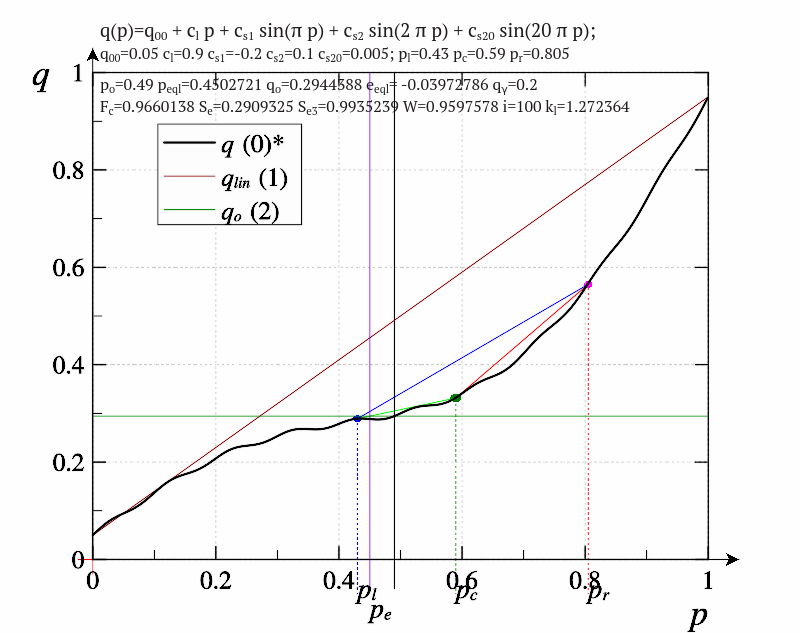
\includegraphics[width=49\TW]{p/pq_sin-p_pq_po=049.png}
    \hfill
    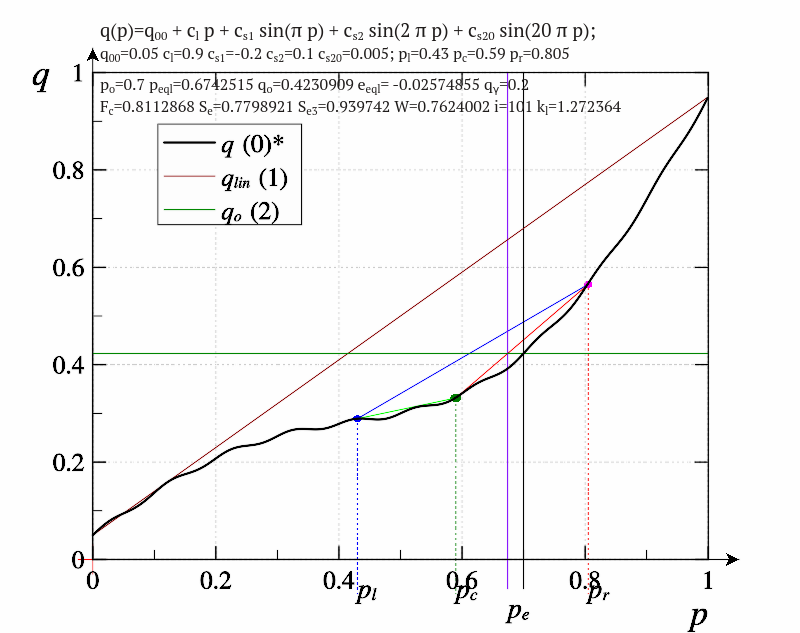
\includegraphics[width=49\TW]{p/pq_sin-p_pq_po=070.png}
  \end{center}
  \caption{Конфігурація точок, відповідні варіанту 4}
  \label{atu:f:pq_4}
\end{figure}

У цьому найсприятливішому випадку проводиться інтерполяція, а не екстраполяція
залежності $q(p)$, і досить вибрати ту ділянку, на якій гарантовано
відбувається перетин. При цьому значення всіх коефіцієнтів підкреслюють
впевненість агента в значенні $p_e$, що отримано:
%
\begin{equation}
  \tilde{p}_e
  =
  \begin{cases}
    \tilde{p}_{el}, & \tilde{q}_l < 0
    \\
    \tilde{p}_{er}, & \text{ otherwise}.
  \end{cases}
  ,
  c_\mathrm{su} = 1.0, \;  c_\mathrm{dist} = 0.5,  \;
  p_b =
  \begin{cases}
    -\tilde{p}_l, & \tilde{q}_l < 0
    \\
    \tilde{p}_r, & \text{ otherwise}.
  \end{cases}.
  \label{atu:eq:pr_e4}
\end{equation}

У будь-якому з розглянутих випадків, має сенс ввести додаткове обмеження на
значення $p_e$, так як через похибки вимірювання і моделювання воно може
виявитися навіть поза діапазону $[p_{\min}, p_{\max}]$. З практичної
точки зору досить добре зарекомендувало себе обмеження
$\tilde {p}_r \in [2 \tilde{p}_l, 2 \tilde{p}_r]$.
З урахуванням низького значення $S$ для
агентів, які потрапили під таке обмеження, їх вплив на загальний результат буде
мінімальним, так як при нормальному перебігу процесу ідентифікації існує хоча б
один агент з високим значенням $S$. Більш суворі обмеження досить рідко
виправдовують себе, так як при цьому не використовуються екстраполяційні
властивості агентів.

Описаний даними правилами спосіб визначення $p_e$ в подальшому будемо
означати як $p_{eql}$\label{atu:d:p_eql}.

\paragraph{Оцінювання впливу оцінки лінійності залежності критерію}

У попередньому аналізі при обчисленні коефіцієнта
``впевненості''~$S$ в розрахунок приймалося тільки відстань від поточних значень
параметрів моделі для
$p_e$. При цьому не враховувалася можливість оцінки лінійності
апроксимації
$q(p)$ за наявними даними. При цьому оцінка повинна бути незалежна
від зміни масштабу як параметрів, так і критеріїв, мати зручну
форму для подальшого використання, і не вимагати обчислень,
занадто чутливих до похибок вимірювання.

Так як в даному випадку один агент спостерігає значення
$p$ і
$q$ для трьох моделей, то оцінити вплив нелінійних факторів він
може в такий спосіб. В першу чергу, за значеннями, відповідним
крайнім точкам лінійною інтерполяцією оцінюється значення
$q_c$ (або ж після нормалізації ---
$ \tilde{q}_c $):
%
\begin{equation}
 q_{c,\mathrm{lin}}
  =
  \frac{  q_l \left( p_r - p_c \right) + q_r \left( p_c - p_l \right) }{p_r-p_l},
  \label{atu:eq:q_clin}
\end{equation}
%
\begin{equation}
  \tilde{q}_{c,\mathrm{lin}}
  =
  \frac{ \tilde{q}_l \tilde{p}_r - \tilde{q}_r \tilde{p}_l }{\tilde{p}_r-\tilde{p}_l}  .
  \label{atu:eq:qr_clin}
\end{equation}

Для забезпечення коректності та малої чутливості отриманих
оцінок до помилок вимірювання слід забезпечити достатню
відстань між сусідніми агентами. Цю вимогу необхідно
враховувати при визначенні динаміки агентів. З іншого боку,
проведення всіх попередніх оцінок величини
$ p_e $ неявно передбачалося
$ \tilde{p}_l <0 $ і
$ \tilde{p}_r> 0 $.

Отже, на початковому етапі роботи методу випадок надмірної
близькості агентів буде виявлятися автоматично і оброблятися
окремо особливим чином. Наприклад, в цьому випадку має сенс
прийняти
$ p_e = p_c $ при збереженні досить високих значень
$ S $ --- якщо метод привів кілька агентів в малий окіл однієї
точки, то або точка дійсно близька до шуканої, або ж весь метод
недостатньо придатний для вирішення поставленого завдання.


З отриманих оцінок
$ q_{c, \mathrm{lin}} $,
$ \tilde{q}_{c, \mathrm{lin}} $
сформуємо такі безрозмірні коефіцієнти, що
дозволяють оцінити нелінійність~$q(p)$:
%
\begin{equation}
  k_l = 1 + \frac{|q_c - q_{c,\mathrm{lin}}|}{|q_r-q_l|} ,
  \label{atu:eq:k_l1}
\end{equation}
%
\begin{equation}
  k_l = 1 + \frac{|\tilde{q}_c - \tilde{q}_{c,\mathrm{lin}}|}{ |\tilde{q}_r-\tilde{q}_l|} .
  \label{atu:eq:k_l2}
\end{equation}

Зазначене подання
$ k_l $ було вибрано з метою безпосереднього використання цієї
величини в
$ S $, тобто якщо
$ \tilde{q}_{c, \mathrm{lin}} \to \tilde{q}_c $, то
$ k_l \to 1 $, і є підстави вважати, що на відстанях порядку
$ p_r-p_l $ оцінка
$ p_e $ достатньо обумовлена. З іншого боку, якщо
$ k_l \gg 1 $, то нелінійні ефекти в даній області переважають над
лінійними, і оцінку
$p_e$ варто розглядати як недостовірну. При практичному
використанні має сенс штучно обмежити цю величину, наприклад
$ k_l <100 $, так як необмежене зростання при прагненні знаменника
до нуля принципово нічого не змінює в роботі методу, але при
цьому можливі проблеми чисто обчислювального характеру.



% }}}2

\subsection{Методи агентів, які використовують значення функції якості}%{{{2

Єдиний нерухомий агент, який використовує значення функції якості, ще більш марний
(з точки зору синтезу системи ідентифікації), ніж один нерухомий агент, який
використовує значення критерію.
%
так як в цьому випадку навіть наявність залежності
$q(p)$ не дає можливості однозначно визначити значення
параметра. Він може сигналізувати про те, що в межах \(\tau \) модель
була чи не була досить адекватна об'єкту.

Наявність історії і можливість переміщатися дають можливість
побудувати систему ідентифікації і з використанням одного агента.
У якості історії
можуть використовуватися, в тому числі, динамічні властивості
ідентифікованого об'єкта
(оригінальний метод адаптивно-пошукової ідентифікації~\cite{mich_92,mich_92}).
Також можуть бути застосовані елементи агента
ідентифікації, яки реалізують усереднення (синхронний детектор та інші).
Застосування методів з однією моделлю вимагає певного механізму
збереження історії процесу пошуку, в межах
одного пошукового ``періоду''. Це сильно обмежує діапазон
застосовності даних методів, в першу чергу --- через значних
часових витрат на пошук, що повторюється у однієї області.

Пара агентів, що взаємодіє між собою, здатна оцінити градієнт функції якості,
і, отже, забезпечити зміщення в потрібному напрямку.
Застосування пари моделей \cite{atu_asau3} (в цьому випадку має сенс
говорити про одного пошуковому агента) дозволяє з меншими
часовими витратами оцінити градієнт функції якості, і,
як наслідок --- визначити значення параметра. Також значною
перевагою такого підходу є менша швидкість зміни параметрів
моделей. Це особливо важно для об'єктів з високою чутливістю
до параметричних збурень.

З урахуванням глобальної інформації можлива адаптація
параметрів пари. У свою чергу, інформація, отримана від пари
може використовуватися для уточнення глобальних параметрів.

Кожен пошуковий агент, визначаючи величину $q_{i}(t)$, і отримуючи $q_o(t)$,
обчислює безрозмірну функцію якості ідентифікації $F (q_o, q_i)$. Як
варіант, агент (або навіть вся керована частина системи ідентифікації) не має
безпосереднього доступу до критерію, і отримує тільки значення~$F$.

Три сусідніх агента, які взаємодіють між собою, здатні не тільки оцінити градієнт
функції якості у власному околі, а й визначити наявність там
максимуму.

На відміну від методів, які використовують значення критерію безпосередньо, в
цьому випадку немає можливості обробляти кожну з пар точок $(p_l, p_c)$ і
$(p_c, p_r)$ незалежно. З трьох точок поблизу $M_{i}$ функція $F(p)$
апроксимується параболою, і абсциса її вершини задає шукане значення параметра.
Змістимо початок координат в точку
$(p_c, F_c)$. Тоді
%
\[
  \tilde{p}_c = 0, \,
  \tilde{p}_l = p_l - p_c, \,
  \tilde{p}_r = p_r - p_c.
\]
%
\[
  \tilde{F}_c = 0, \,
  \tilde{F}_l = F_l - F_c, \,
  \tilde{F}_r = F_r - F_c.
\]
%
\[
  \left\{
    \begin{array}{l}
      a_2 \tilde{p}_l^2 + a_1 \tilde{p}_l  = \tilde{F}_l
      \\
      a_2 \tilde{p}_r^2 + a_1 \tilde{p}_r  = \tilde{F}_r
    \end{array}
  \right. .
\]
%
\[
  a_1 = \frac{\tilde{F}_r \tilde{p}_l^2 - \tilde{F}_l \tilde{p}_r^2 }
             { \tilde{p}_l^2 \tilde{p}_r  - \tilde{p}_l \tilde{p}_r^2 }.
\]
%
\[
  a_2 = - \frac{\tilde{F}_r \tilde{p}_l - \tilde{F}_l \tilde{p}_r }
               { \tilde{p}_l^2 \tilde{p}_r  - \tilde{p}_l \tilde{p}_r^2 }.
\]

\begin{equation}
  \tilde{p}_e = - \frac{a_1}{2 a_2};
  \;
  p_e = p_c - \frac{a_1}{2 a_2}.
  \label{atu:eq:p_eFq}
\end{equation}

При цьому, якщо
$a_2 \ge 0$,
то ця ситуація аналогічна випадку 2C метода $p_{eql}$~(см.~стр.~\pageref{atu:d:p_eql_2A}),
що потребує обмеження $p_e$ та корекції величин $c_\mathrm{su}$ та $c_\mathrm{dist}$.

Визначення $p_e$ по (\ref{atu:eq:p_eFq}) будемо позначати як $p_{eFq}$.

Розглянемо роботу цього методу при тих же умовах, при яких
ілюструвався метод
$p_{eql}$. Перш за все проілюструємо варіант, коли центральна точка
--- найгірша~(рис.~\ref{atu:f:p_eFq_bad}).


\begin{figure}[htb!]
  \begin{center}
    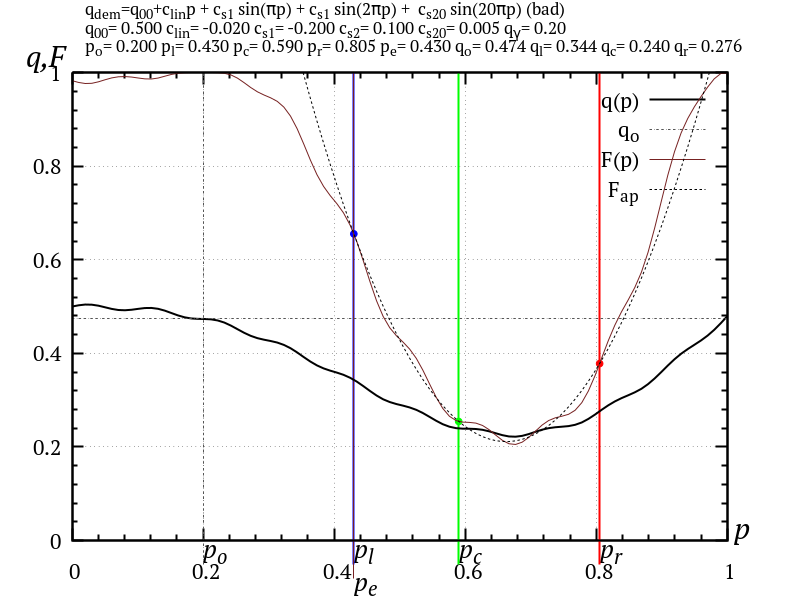
\includegraphics[width=60\TW]{p/p_eFq/q_p_eFq_bad.png}
  \end{center}
  \caption{Визначення точки $ p_e $ методом$ p_{eFq} $ в найгіршому випадку}
  \label{atu:f:p_eFq_bad}
\end{figure}

Як видно з графіка, в цьому випадку апроксимація залежності
$ F (p) $ параболою
$ F_{ap} (p) $ досить точна, але позитивна визначеність величини
$ a_2 $ показує, що знайдений екстремум відповідає мінімуму, що
абсолютно не допомагає у визначенні
$ p_e $. У той же час, дія методу в цьому випадку --- вибір однієї з
граничних точок правильно вказує напрямок.

Протилежний випадок, коли центральна точка --- найкраща, але все
ж недостатньо, представлений на рис.~\ref{atu:f:p_eFq_good}.

\begin{figure}[htb!]
  \begin{center}
    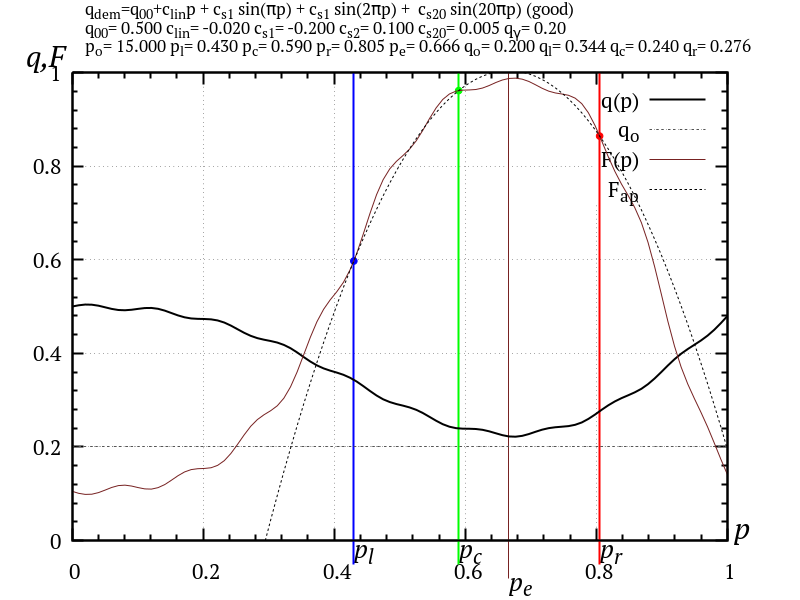
\includegraphics[width=60\TW]{p/p_eFq/q_p_eFq_good.png}
  \end{center}
  \caption{Визначення точки $ p_e $ методом $ p_{eFq} $ в разі, коли центральна точка --- найкраща, але немає перетину $q(p)$ з $ q_o $}
  \label{atu:f:p_eFq_good}
\end{figure}

На відміну від методу
$ p_{eql} $, для розглянутого методу цей випадок не є
особливим. Знайдене значення
$ p_e $ досить добре відповідає точці, в якій
$q(p)$ максимально наближається до
$ q_o $. Це цілком розумна поведінка, з урахуванням того, що при
наближенні до цієї точки, за уточненими даними може бути
знайдено те
$ q (p) = q_o $. З іншого боку, це може бути локальний екстремум, який
не відповідає згаданої значенням
$ p_o $, як і представлено в цьому прикладі.

Приклад невизначеного випадку, коли на робочому інтервалі є
два перетину
$ q (p) $ з
$ q_o $, представлений на рис.~\ref{atu:f:p_eFq_double}.

\begin{figure}[htb!]
  \begin{center}
    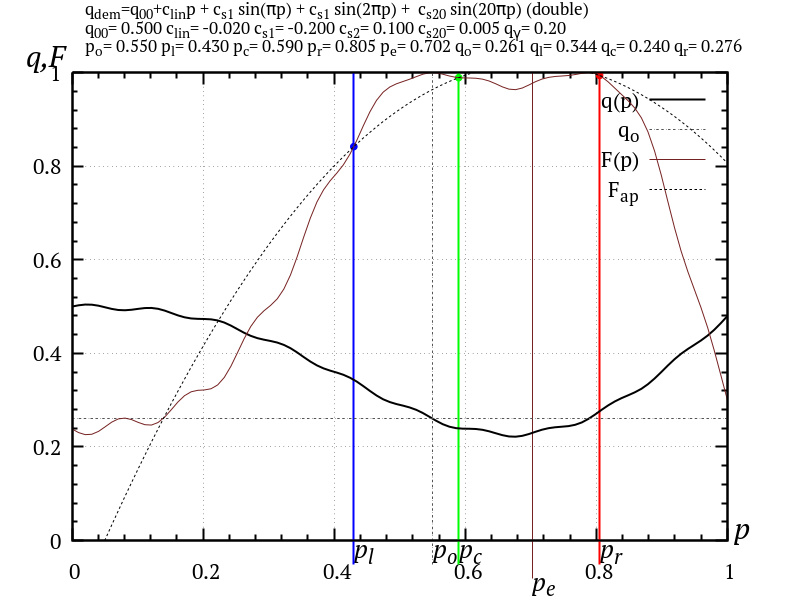
\includegraphics[width=60\TW]{p/p_eFq/q_p_eFq_double.png}
  \end{center}
  \caption{Визначення точки $ p_e $ методом $ p_{eFq} $ в разі двох перетинів $ q (p) $ з $ q_o $}
  \label{atu:f:p_eFq_double}
\end{figure}

Невизначеність умови не дозволяє вибрати будь-яку певну і
найкращу в будь-якому випадку поведінку системи. В даному конкретному
випадку був обраний варіант, що веде значення $p_e$ у бік від вихідного
$p_o$. Більш того, на відміну від методу
$ p_{eql} $, алгоритмічно даний випадок виділити неможливо,
спираючись лише на значення функції якості. Як результат ---
немає можливості зазначити цей випадок зниженням величини
$S$.

Розглянемо більш певний випадок, для якого метод
$p_{eql}$ отримував оцінку
$ p_e $ шляхом екстраполяції (рис.~\ref{atu:f:p_eFq_extra}).

\begin{figure}[htb!]
  \begin{center}
    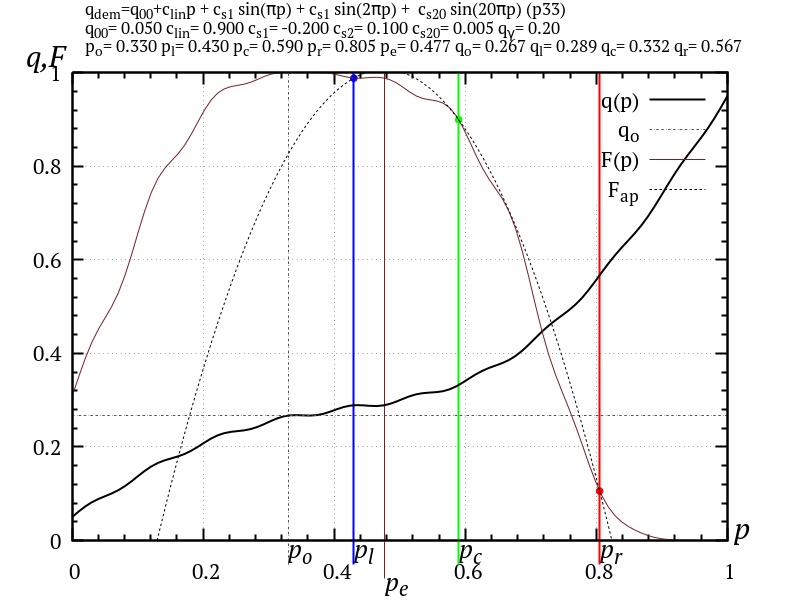
\includegraphics[width=49\TW]{p/p_eFq/q_p_eFq_p33.png}
    \hfill
    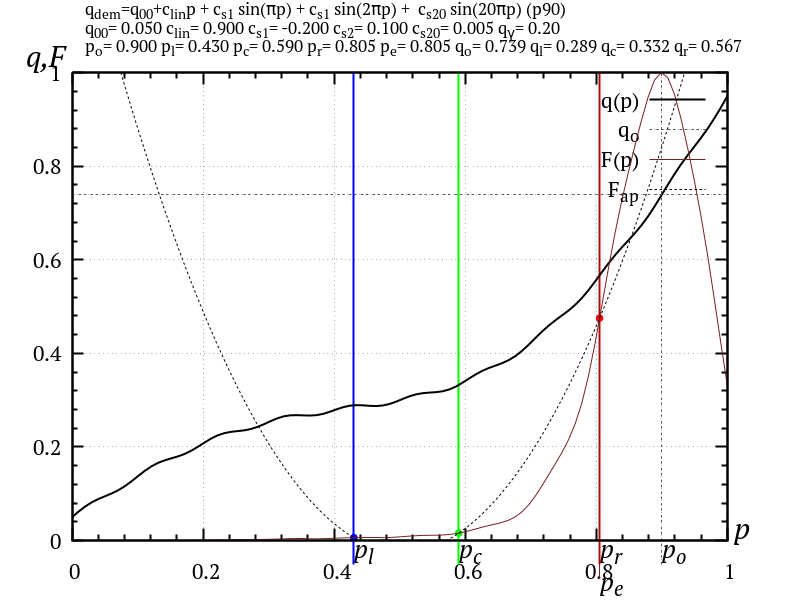
\includegraphics[width=49\TW]{p/p_eFq/q_p_eFq_p90.png}
  \end{center}
\caption{Визначення точки $ p_e $ методом $ p_{eFq} $ при екстраполяції за межі $ [p_l, p_r] $}
\label{atu:f:p_eFq_extra}
\end{figure}

Тут спостерігаються суттєві відмінності від методу
$p_{eql}$. Перш за все, поведінка попереднього методу в цьому,
досить простому випадку, була досить однозначною. Досить було
за заданими правилами зменшувати величину
$S$ при видаленні від робочого інтервалу, для відображення
зменшення ступеня впевненості в отриманому значенні.

Даний метод, як видно на представлених графіках, в східних
випадках може давати абсолютно різні результати. Перший графік,
відповідний
$ p_o = 0.33 $, демонструє не тільки значну похибку ідентифікації,
а й той факт, що немає можливості відокремити цей випадок від
найбільш сприятливого, при
$ p_o \in [p_l, p_r] $. Другий графік ($ p_o = 0.9 $),
хоча вихідні умови принципово не відрізняються від
першого, реалізує умови
$ a_2 \ge 0 $, тобто неможливість визначити
$ p_e $ за рахунок апроксимації другого порядку, і отже, змушує як
наближення використовувати
$ p_r $.

Метод в найбільш сприятливому випадку, при
$p_o \in [p_l,p_r]$, представлено на рис.~\ref{atu:f:p_eFq_intra}.


\begin{figure}[htb!]
  \begin{center}
    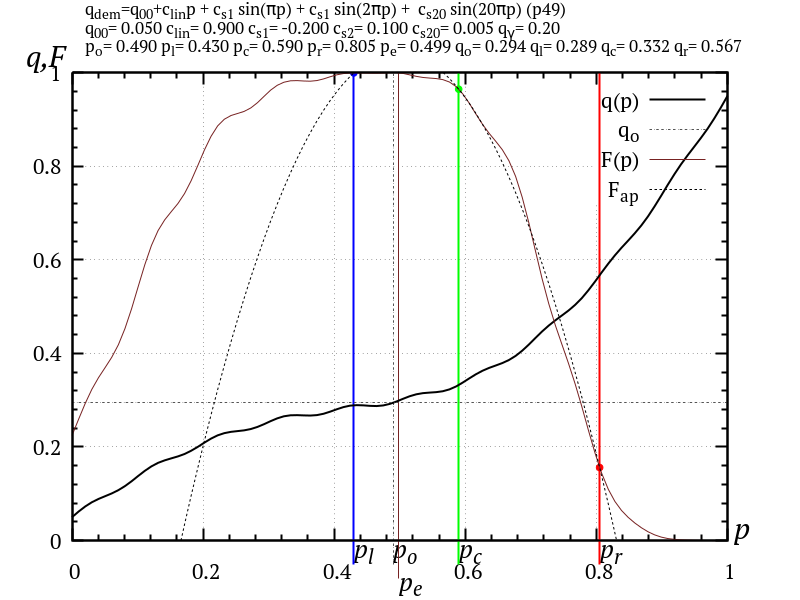
\includegraphics[width=49\TW]{p/p_eFq/q_p_eFq_p49.png}
    \hfill
    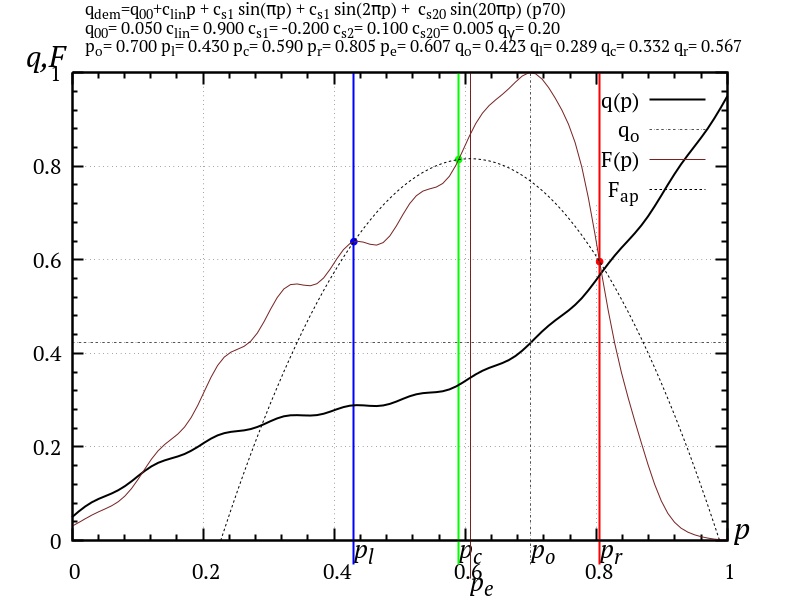
\includegraphics[width=49\TW]{p/p_eFq/q_p_eFq_p70.png}
  \end{center}
\caption{Визначення точки $ p_e $ методом $ p_{eFq} $ при $ p_o \in [p_l, p_r] $}
  \label{atu:f:p_eFq_intra}
\end{figure}

Як і слід було очікувати, оцінка $p_e$ в цьому випадку цілком спроможна, не
дивлячись на те, що в подібних умовах спостерігається різний рівень похибки
ідентифікації.

Розглянемо вплив на працездатність даного методу чутливості
функції якості, яка визначається величиною
$ q_\gamma$. Початкове значення цієї величини
($ q_\gamma = 0.2$) для тестового завдання було підібрано
експериментально~\cite{atu_asau22}. Розглянемо зміну результатів
роботи методу в при
$ p_o \in [p_l, p_r] $ в умовах сильно завищеною чутливості
$ q_\gamma = 0.05 $ (рис.~\ref{atu:f:p_eFq_intra_005}).


\begin{figure}[htb!]
  \begin{center}
    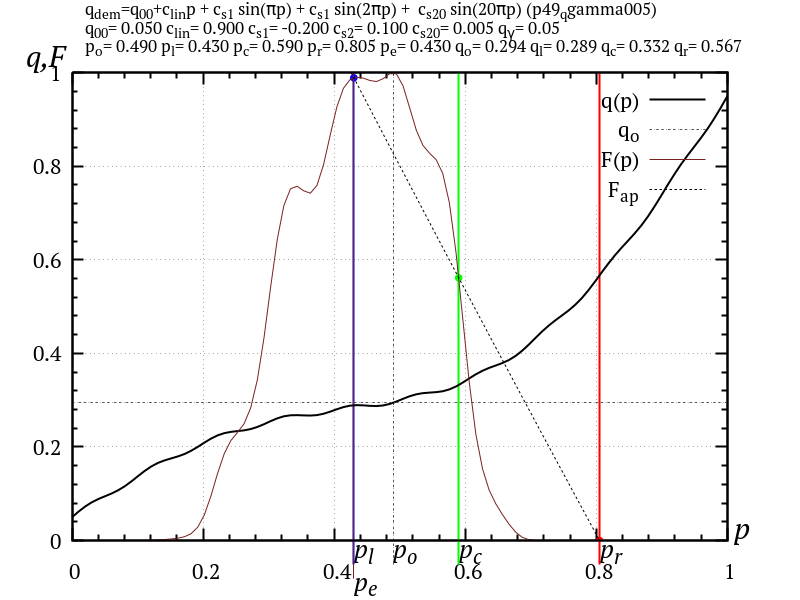
\includegraphics[width=49\TW]{p/p_eFq/q_p_eFq_p49_qgamma005.png}
    \hfill
    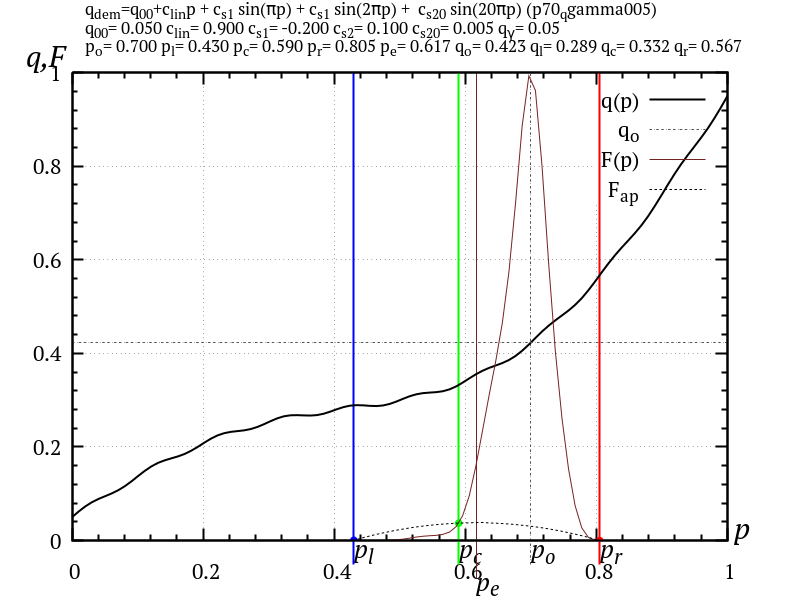
\includegraphics[width=49\TW]{p/p_eFq/q_p_eFq_p70_qgamma005.png}
  \end{center}
\caption{Визначення точки $ p_e $ методом $ p_{eFq} $ при підвищеній чутливості функції якості}
  \label{atu:f:p_eFq_intra_005}
\end{figure}

Цій метод демонструє суттєву чутливість до значення $q_\gamma$.
Зайва чутливість призводить до того, що функція якості є відмінною від нуля в
дуже вузькому діапазоні значень параметра, що призводить до практичної
марності апроксимації і неадекватним результатам
ідентифікації.

Істотно інші результати показує метод в умовах недостатньої
чутливості, що відповідає відносно великим значенням
$q_\gamma$ (рис.~\ref{atu:f:p_eFq_intra_200}).

\begin{figure}[htb!]
  \begin{center}
    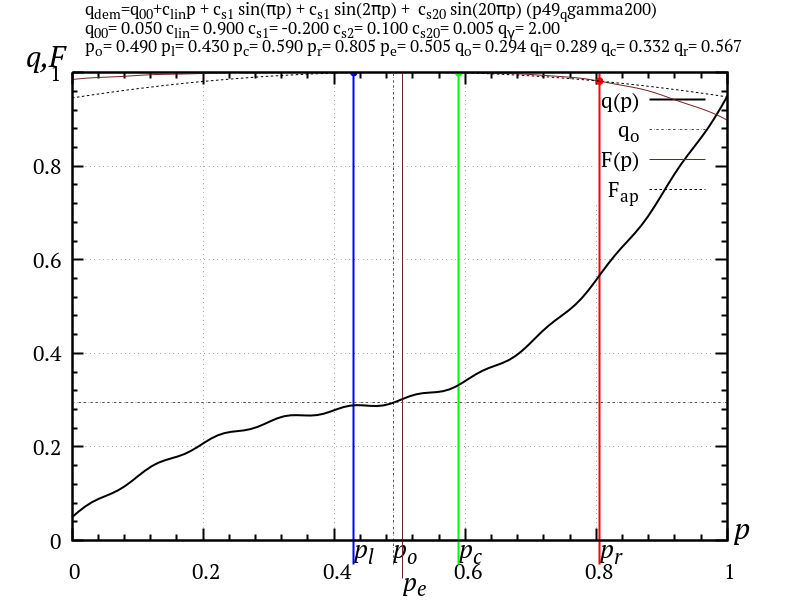
\includegraphics[width=49\TW]{p/p_eFq/q_p_eFq_p49_qgamma200.png}
    \hfill
    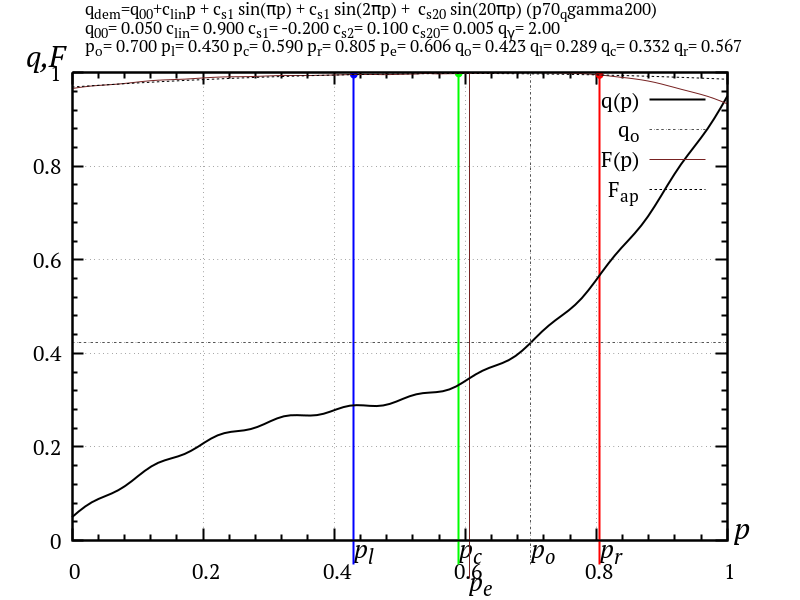
\includegraphics[width=49\TW]{p/p_eFq/q_p_eFq_p70_qgamma200.png}
  \end{center}
\caption{Визначення точки $ p_e $ методом $p_{eFq}$ при недостатній чутливості функції якості}
\label{atu:f:p_eFq_intra_200}
\end{figure}

Досить дивним є той факт, що при значному зменшенні чутливості похибка
ідентифікації росте дуже слабо. В першу чергу це пов'язано з тим, що в цих
умовах сама апроксимація кривої $F$ параболою стає більш точною. Для інших
видів функції якості це не так. Більш того, наведені приклади розраховувалися
за умови відсутності помилок вимірювання. При недостатній чутливості
$F_l \approx F_c \approx F_r \approx 1$, і малі зміни $F$ приведуть до значної
похибки ідентифікації.

В цілому, на підставі отриманих результатів, даний метод демонструє дещо
гірші результати, ніж $p_{eql}$.

Найбільш серйозним недоліком слід вважати неможливість в цьому
випадку адекватним чином визначити величину
$S$, яка на рівні координатора пошуку дозволяє вибрати найбільш
значущих агентів, а на рівні агента --- уникнути надмірної
динаміки далеко від
$ p_o $. Другим за важливістю недоліком є необхідність коректної
настройки величини
$ q_\gamma $, нехай і в досить широких межах. Серед переваг методу
слід відзначити більш просту алгоритмічну організацію, що може
бути істотно при реалізації системи ідентифікації в умовах з
обмеженим обчислювальними ресурсами.



\paragraph{Визначення $ p_e $ методом COG за значеннями функції якості в 3 точках}

Досить простим і маловитратними з точки зору обчислень є метод оцінювання $p_e$ методом
COG (Center Of Gravity) за значеннями функції якості:
%
\begin{equation}
  p_e =
  \frac{p_l F_l + p_c F_c + p_r F_r}{ F_r + F_c + F_r}  .
  \label{atu:eq:p_eFc}
\end{equation}

Умова обмеженості оцінки $p_e \in [p_l; p_r]$ в цьому випадку виконується
автоматично.
Єдина складність --- обробка особливого випадку для тих видів
$F(q) $, які звертаються в нуль на видаленні від центральної
точки. В цьому випадку знаменник (\ref{atu:eq:p_eFc}) звертається в нуль,
а в якості $ p_e $ має сенс вибрати $ p_c $.
Для тих видів функцій якості, які не приймають строго
нульових значень, формально такої проблеми немає.
Але в заданих умовах цей метод занадто
сильно піддається впливу перешкод вимірювання.

Для цього способу не представляється можливим досить корисним
способом визначити величину
$ S $, тому, для збереження однаковості покладемо
$ S = 1 $.

Визначення $p_e$ по (\ref{atu:eq:p_eFc}) в подальшому будемо позначати $p_{eFc}$.


% }}}2

\subsection{Оцінка працездатності та ефективності методів оцінювання ідентифікованого параметра одним пошуковим агентом} % {{{2

Для визначення працездатності і властивостей різних методів оцінювання $p_e$
в контрольованих умовах без урахування динаміки агентів була обрана наступна
тестова задача: залежність $q (p)$ визначалася по (\ref{atu:eq:q_dem}),
$p_{\min}=20$, $p_{\max}=60$,
$q_{00}=7$, $c_\mathrm{lin}=-4.0$.
Початкове розташування агентів рівномірне і штучно зафіксоване:
$p_l=30$, $p_c=40$,  $p_r=50$.

Значення коефіцієнтів
$c_\mathrm{s1}$, $c_\mathrm{s2}$, $c_\mathrm{s20}$
вибиралися по одному з трьох наборів:
%
\begin{equation}
  c_\mathrm{s1} = 0.2, c_\mathrm{s2} = -0.4, c_\mathrm{s20} = 0.02,
  \label{atu:eq:q_dem_all}
\end{equation}
%
\begin{equation}
  c_\mathrm{s1} = 0, c_\mathrm{s2} = 0, c_\mathrm{s20} = 0.02,
  \label{atu:eq:q_dem_s20}
\end{equation}
%
\begin{equation}
  c_\mathrm{s1} = c_\mathrm{s2} = c_\mathrm{s20} = 0 .
  \label{atu:eq:q_dem_lin}
\end{equation}

При цьому набір параметрів (\ref{atu:eq:q_dem_all}) дозволяє досліджувати
поведінку похибки ідентифікації при впливі як низькочастотних,
так і високочастотних нелінійних компонент,
(\ref{atu:eq:q_dem_s20}) ---
тільки високочастотних,
а (\ref{atu:eq:q_dem_lin})
реалізує простий лінійний випадок.

\begin{figure}[htb!]
  \begin{center}
    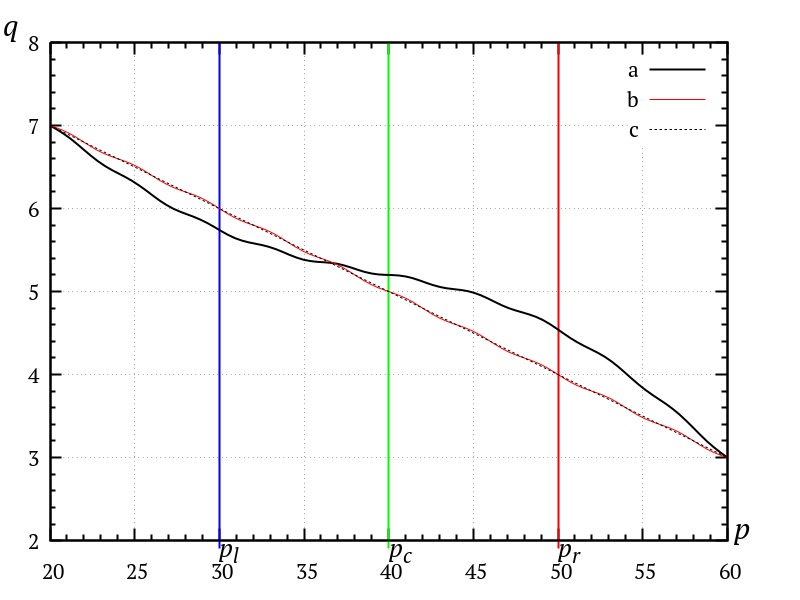
\includegraphics[width=0.7\textwidth]{p/q_p_dem.png}
  \end{center}
  \caption{Вид тестової функції $q_\mathrm{dem}(p)$:
     a --- умови (\ref{atu:eq:q_dem_all}),
     b --- умови (\ref{atu:eq:q_dem_s20}),
     c --- умови (\ref{atu:eq:q_dem_lin})
  }
  \label{atu:f:q_dem}
\end{figure}

У першій серії обчислювальних експериментів значення параметра об'єкта $p_o$
змінювалося в діапазоні $[p_{\min}; p_{\max}]$ при фіксованій відстані
між агентами $A = p_c - p_l = p_r - p_c$. Це дозволило оцінити як
інтерполяційні (при $p_o \in [p_l, p_r]$), так і екстраполяційні можливості
методів. Так як частина методів при визначенні $p_e$ використовує значення
функції якості, то при проведенні експериментів величина $q_\gamma$ також
варіювалася.

Для методу
$ p_{eql} $ безпосередній залежності від цієї величини немає, але
для однаковості представлених результатів все графіки наведені
як залежності від
$ p_o $ і
$ q_\gamma $. Всі представлені графіки, для зручності порівняння,
виконані в одному масштабі і однієї і тієї ж проекції. Масштаб
по осі
$ Z $, що використовується для представлення модуля похибки
ідентифікації, був обраний
$ Z_{\max} = A / 2 = 5 $ для наочного порівняння з відстанню між агентами,
при цьому величини, більші ніж
$A/2$ відповідають невиправдано великий похибці, і знаходяться
за межами графіка.

На рис.~\ref{atu:f:qsl_pe_po_qg_all} подані залежності помилок
ідентифікації для тестового завдання (\ref{atu:eq:q_dem}) при повному
комплекті нелінійних членів  трьома нерухомими
агентами трьома розглянутим методами визначення $p_e$.

\begin{figure}[htb!]
  \begin{center}
    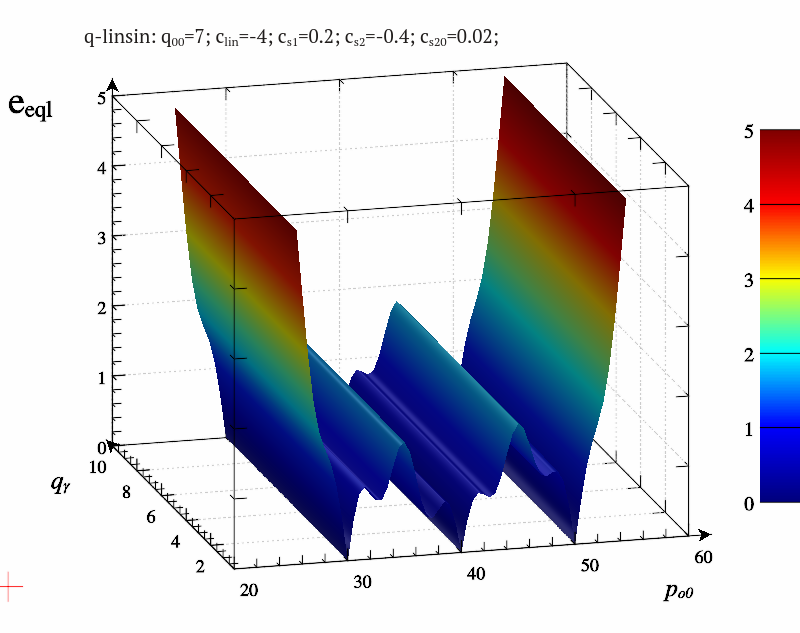
\includegraphics[width=0.32\textwidth]{p/qls_pe-p_po_qg_eql_all.png}
    \hfill
    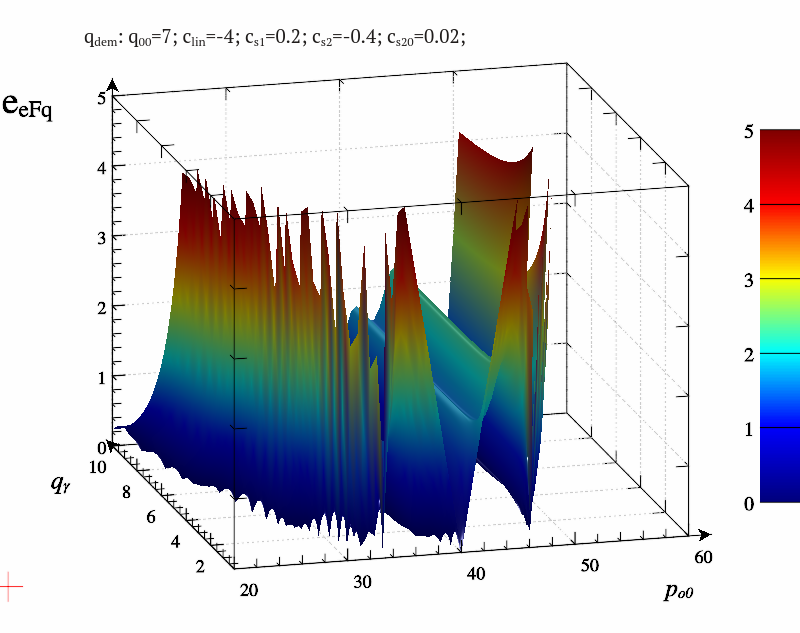
\includegraphics[width=0.32\textwidth]{p/qls_pe-p_po_qg_eFq_all.png}
    \hfill
    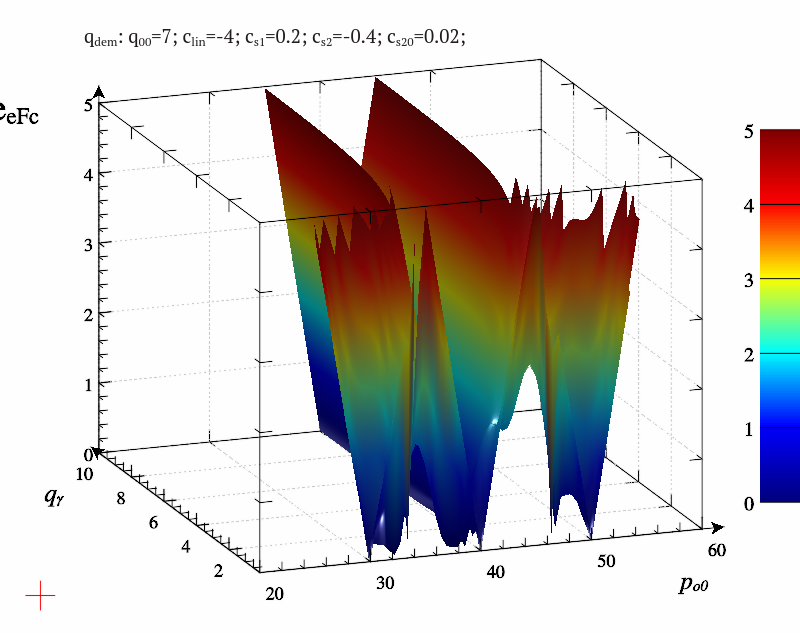
\includegraphics[width=0.32\textwidth]{p/qls_pe-p_po_qg_eFc_all.png}
  \end{center}
  \vspace{-1.0ex}
  \begin{center}
    ~ \hfill a \hfill\hfill b \hfill\hfill c \hfill ~
  \end{center}
  \vspace{-1.5ex}
  \caption{Залежності $e(p_o,q_\gamma)$ для методів $p_{eql}$ (a), $p_{eFq}$ (b), $p_{qFc}$ (c) за умов (\ref{atu:eq:q_dem_all})}
  \label{atu:f:qsl_pe_po_qg_all}
\end{figure}

Метод $p_{eql}$ демонструє досить обмежену похибку ідентифікації при
$p_o \in [p_l; p_r]$, і досить швидке, але лінійно обмежене зростання похибки за
межами цього робочого діапазону. Метод $p_{eFq}$ має істотну залежність
від величини $q_\gamma$: малі значення призводять до суттєвого
зростання похибки, а з подальшим зростанням рівень похибки в межах робочого
діапазону приблизно одного порядку з похибкою в методі $p_{eql}$. При
цьому, за межами робочого діапазону спостерігається більш суттєве зростання
похибки. Метод $p_{qFc}$ демонструє задовільні результати тільки в дуже
вузькому діапазоні значень $q_\gamma$, що ставить під серйозний сумнів
можливість застосування цього методу для реальних задач, оскільки при цьому
немає можливості передбачити таке значення цього параметра, при якому метод буде
працездатний.


На рис.~\ref{atu:f:qsl_pe_po_qg_s20} представлені аналогічні залежності
помилок ідентифікації, але з нелінійних членів залишений самий
високочастотний~(\ref{atu:eq:q_dem_s20}).

\begin{figure}[htb!]
  \begin{center}
    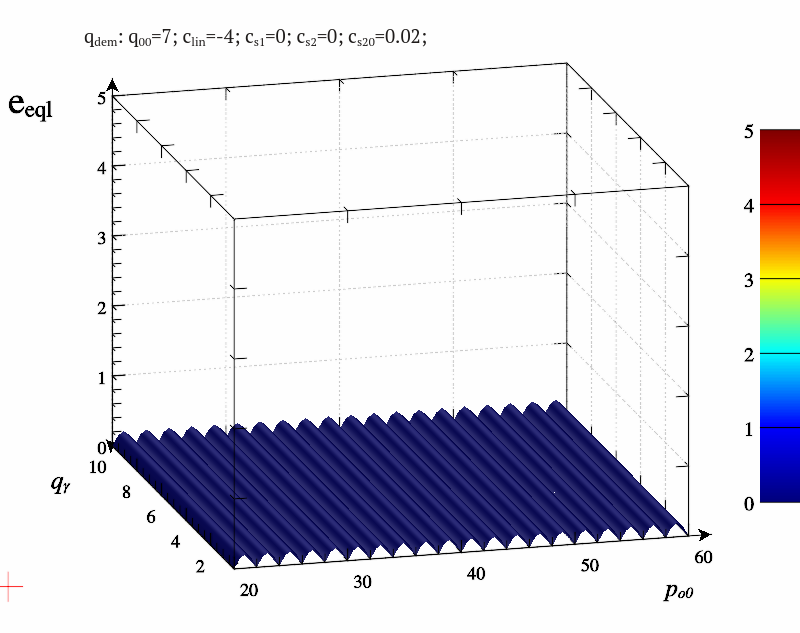
\includegraphics[width=0.32\textwidth]{p/qls_pe-p_po_qg_eql_s20.png}
    \hfill
    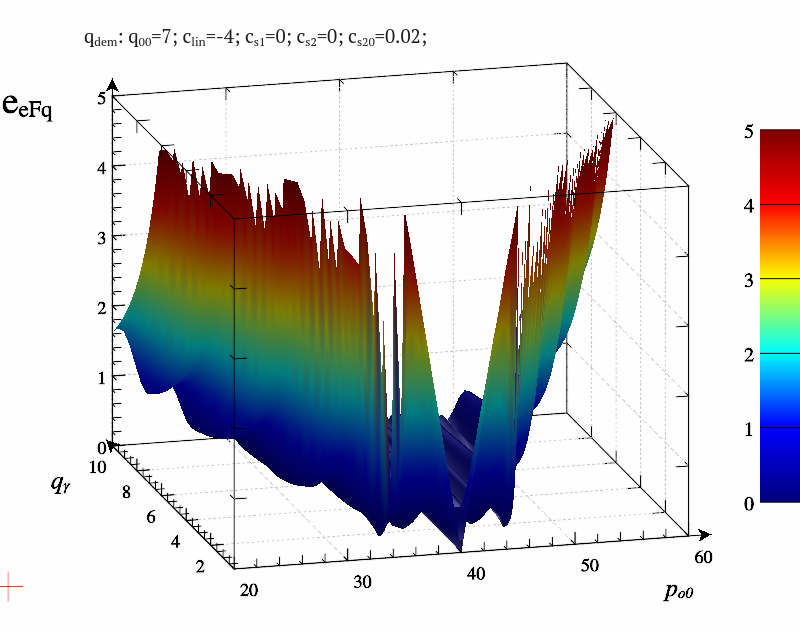
\includegraphics[width=0.32\textwidth]{p/qls_pe-p_po_qg_eFq_s20.png}
    \hfill
    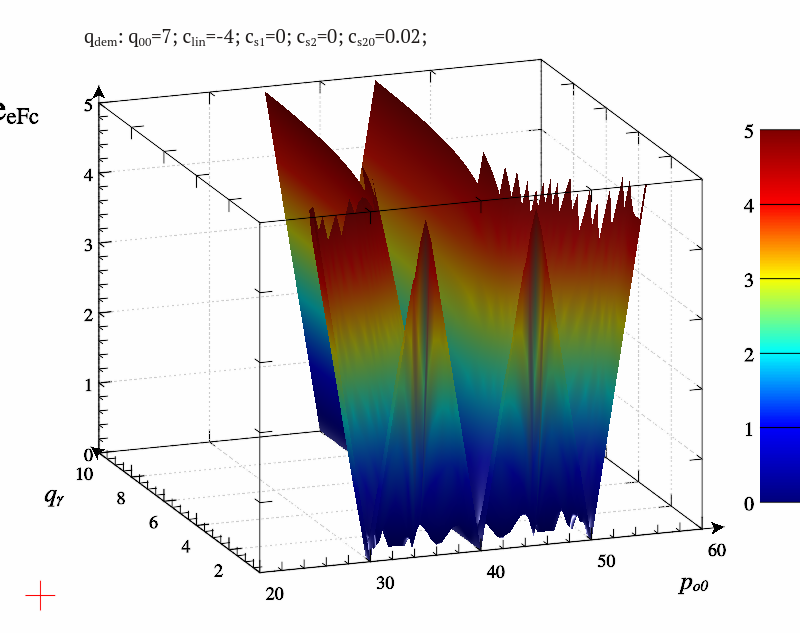
\includegraphics[width=0.32\textwidth]{p/qls_pe-p_po_qg_eFc_s20.png}
  \end{center}
  \vspace{-1.0ex}
  \begin{center}
    ~ \hfill a \hfill\hfill b \hfill\hfill c \hfill ~
  \end{center}
  \vspace{-1.5ex}
  \caption{Залежності $e(p_o,q_\gamma)$ для методів $p_{eql}$ (a), $p_{eFq}$ (b), $p_{qFc}$ (c) за умов (\ref{atu:eq:q_dem_s20})}
  \label{atu:f:qsl_pe_po_qg_s20}
\end{figure}

У цих умовах метод
$ p_{eql} $ демонструє результати, близькі до ідеальних, дрібні
``брижі'' на поверхні похибки відповідають малим періодичним
збуренням
$q(p)$, а в цілому навіть екстраполяція не приводить до зростання
похибки. В якійсь мірі це обумовлено тим, що на робочий діапазон
доводиться ціле число періодів збурення. Залежність похибки
для методу
$ p_{eFq} $ проявляє менше значення помилок для тих ділянок, де
і спостерігався невеликий рівень помилок для попереднього
випадку, і практично незмінний --- за межами цієї
області. Принципової різниці в поведінці методу
$ p_{qFc} $ в порівнянні з попереднім випадком немає.

На рис.~\ref{atu:f:qsl_pe_po_qg_lin} представлені ті ж залежності, але в
тривіальному випадку (\ref{atu:eq:q_dem_lin}), коли залежність
$q(p) $ лінійна.

\begin{figure}[htb!]
  \begin{center}
    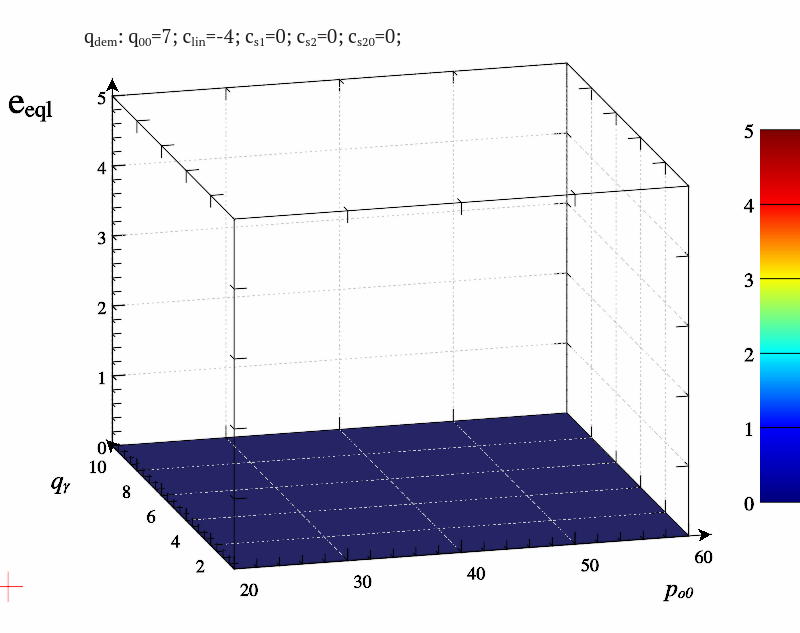
\includegraphics[width=0.32\textwidth]{p/qls_pe-p_po_qg_eql_lin.png}
    \hfill
    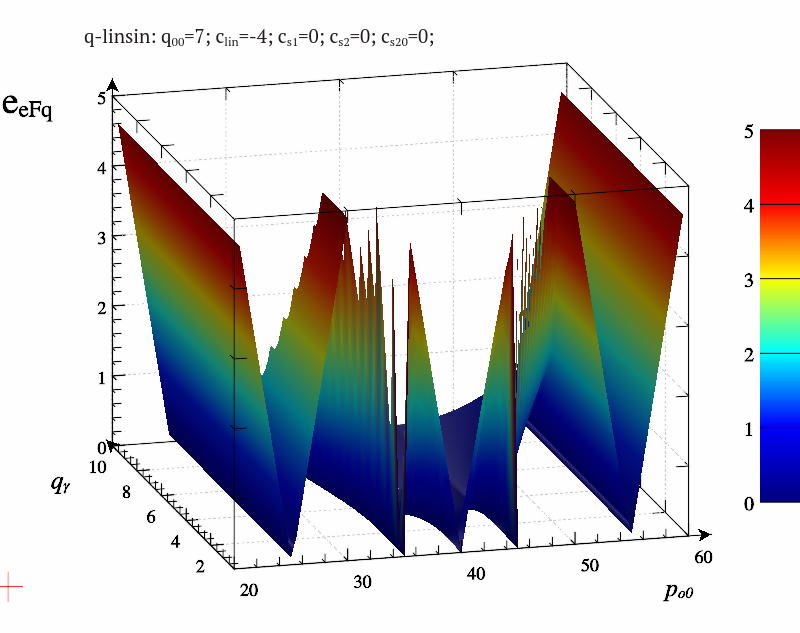
\includegraphics[width=0.32\textwidth]{p/qls_pe-p_po_qg_eFq_lin.png}
    \hfill
    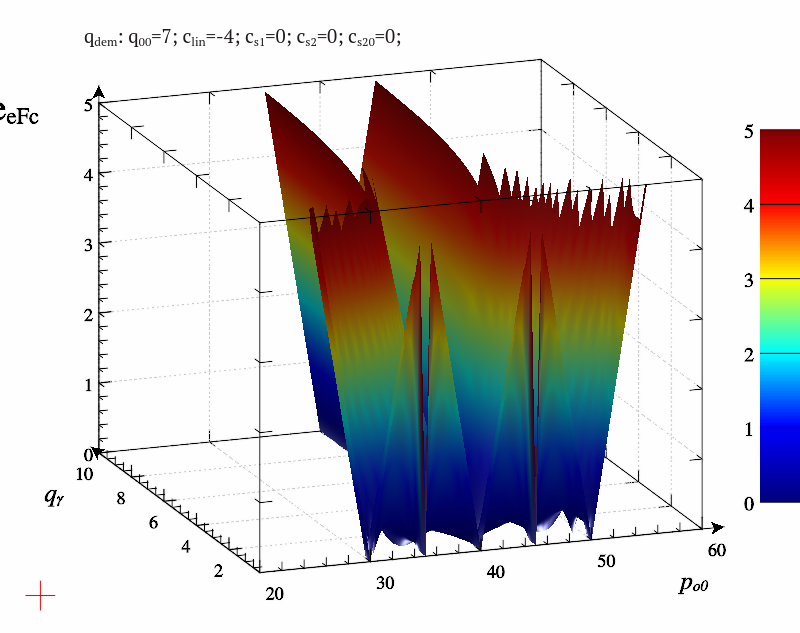
\includegraphics[width=0.32\textwidth]{p/qls_pe-p_po_qg_eFc_lin.png}
  \end{center}
  \vspace{-1.0ex}
  \begin{center}
    ~ \hfill a \hfill\hfill b \hfill\hfill c \hfill ~
  \end{center}
  \vspace{-1.5ex}
  \caption{Залежності $e(p_o,q_\gamma)$ для методів $p_{eql}$ (a), $p_{eFq}$ (b), $p_{qFc}$ (c) за умов (\ref{atu:eq:q_dem_lin})}
  \label{atu:f:qsl_pe_po_qg_lin}
\end{figure}

Як і слід було очікувати, метод
$p_{eql}$ демонструє ідеальні результати. Графік залежності для
методу
$ p_{eFq} $ окреслює його діапазон застосовності --- незважаючи на
лінійність
$q(p)$ метод стає непрацездатним при надмірно чутливої
функції якості. І нарешті, поверхня графіку для методу
$p_{eFc}$, що виглядає практично однаково для всіх розглянутих варіантів,
підтверджує його слабку придатність.


На рис.~\ref{atu:f:qsl_S_po_qg_all} подані залежності
$S (p_o, q_\gamma)$
при тих же умовах, при яких було отримано рис.~\ref{atu:f:qsl_pe_po_qg_all}.
Використовувалося визначення (\ref{atu:eq:S3}), як
потенційно більш адекватне похибці ідентифікації.

\begin{figure}[htb!]
  \begin{center}
    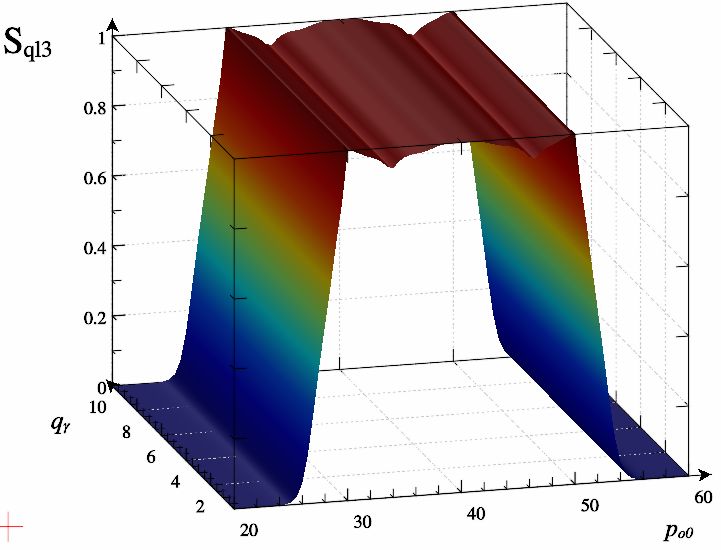
\includegraphics[width=0.32\textwidth]{p/qls_pe-p_po_qg_Sql_all_xl.png}
    \hfill
    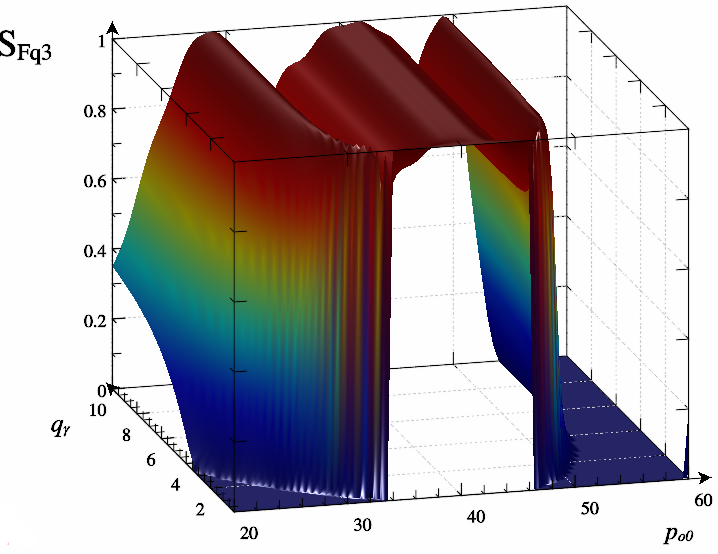
\includegraphics[width=0.32\textwidth]{p/qls_pe-p_po_qg_SFq_all_xl.png}
    \hfill
    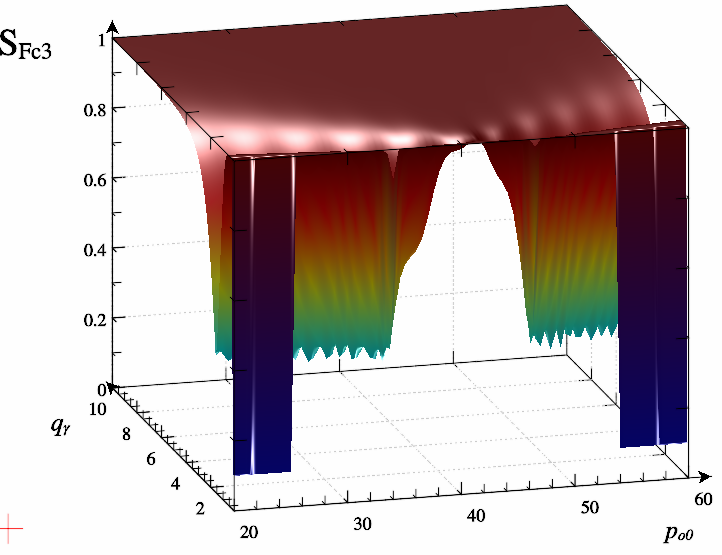
\includegraphics[width=0.32\textwidth]{p/qls_pe-p_po_qg_SFc_all_xl.png}
  \end{center}
  \vspace{-1.0ex}
  \begin{center}
    ~ \hfill a \hfill\hfill b \hfill\hfill c \hfill ~
  \end{center}
  \vspace{-1.5ex}
  \caption{Залежності $S(p_o,q_\gamma)$ для методів $p_{eql}$ (a), $p_{eFq}$ (b), $p_{qFc}$(c) за умов (\ref{atu:eq:q_dem_all})}
  \label{atu:f:qsl_S_po_qg_all}
\end{figure}

Для методу $p_{eql}$ близькі до одиниці значення $S$, як і планувалося,
спостерігаються в тих же областях, де і низький рівень похибки ідентифікації, в
першу чергу --- всередині робочого діапазону. При цьому, ця величина не є
прямим відображення рівня похибки, оскільки це неможливо визначити за трьома точкам.
Метод $p_{eFq}$ також характеризується досить коректним видом цієї залежності,
включаючи низький рівень впевненості при підвищеній чутливості функції якості.
Навпаки, для методу $p_{eFc}$ графік показує, що для нього це визначення $S$ не має сенсу.


На рис.~\ref{atu:f:qsl_S_po_qg_s20} представлені аналогічні залежності,
але з нелінійних членів залишений самий високочастотний~(\ref{atu:eq:q_dem_s20}).

\begin{figure}[htb!]
  \begin{center}
    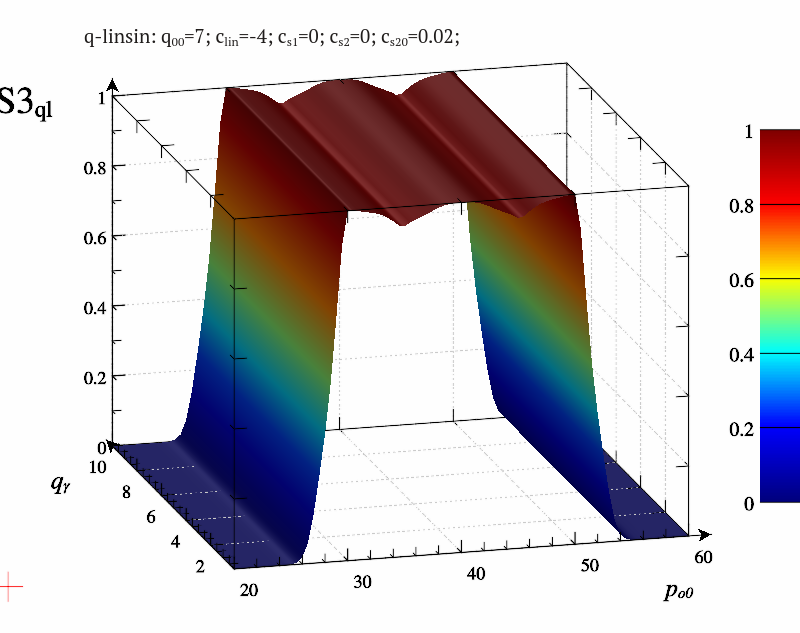
\includegraphics[width=0.32\textwidth]{p/qls_pe-p_po_qg_Sql_s20.png}
    \hfill
    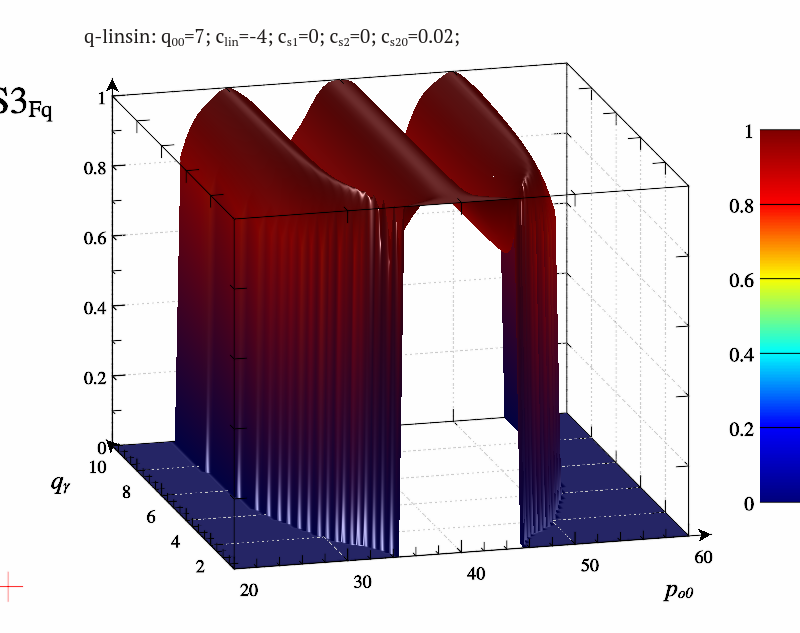
\includegraphics[width=0.32\textwidth]{p/qls_pe-p_po_qg_SFq_s20.png}
    \hfill
    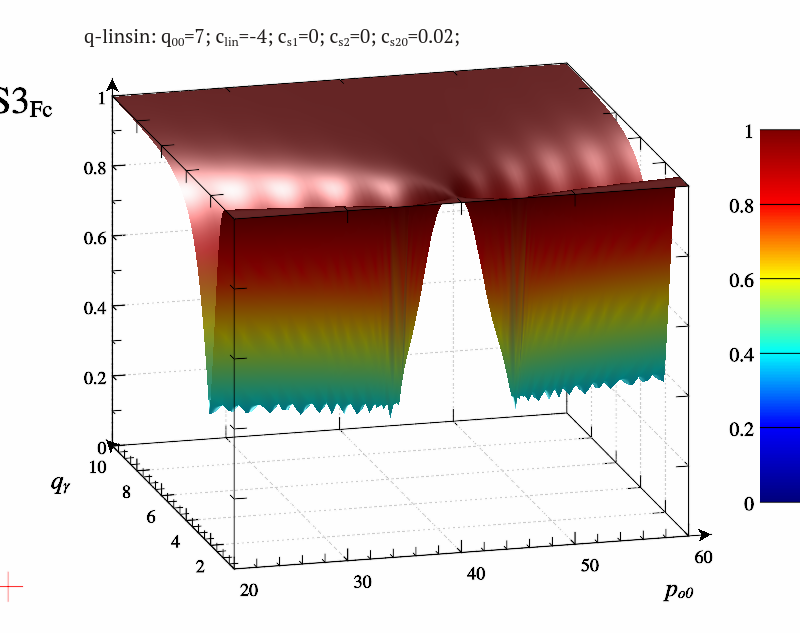
\includegraphics[width=0.32\textwidth]{p/qls_pe-p_po_qg_SFc_s20.png}
  \end{center}
  \vspace{-1.0ex}
  \begin{center}
    ~ \hfill a \hfill\hfill b \hfill\hfill c \hfill ~
  \end{center}
  \vspace{-1.5ex}
  \caption{Залежності $S(p_o,q_\gamma)$ для методів $p_{eql}$ (a), $p_{eFq}$ (b), $p_{qFc}$ (c) за умов (\ref{atu:eq:q_dem_s20})}
  \label{atu:f:qsl_S_po_qg_s20}
\end{figure}

У порівнянні з попереднім випадком, графік для методу
$ p_{eql} $ має набагато більший радіус дії, при збереженні загальної
форми. Це пов'язано з тим, що для даного випадку
$ k_l = 1 $, діапазон впевненого визначення
$ p_e $ відповідно розширюється, що навіть надмірно
підтверджується не зростаючим рівнем похибок. Зміни для методу
$ p_{qFq} $ не такі помітні, так як для нього не враховується оцінка
рівня лінійності. Для методу
$ p_{eFc} $ зберігається майже безглузда залежність.

На рис.~\ref{atu:f:qsl_S_po_qg_lin} представлені ті ж залежності,
але в лінійному випадку (\ref{atu:eq:q_dem_lin}).

\begin{figure}[htb!]
  \begin{center}
    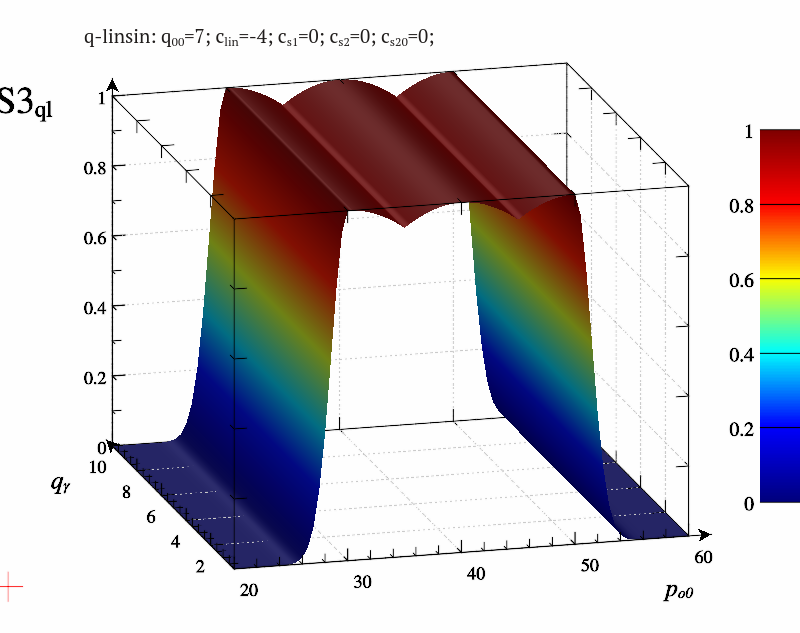
\includegraphics[width=0.32\textwidth]{p/qls_pe-p_po_qg_Sql_lin.png}
    \hfill
    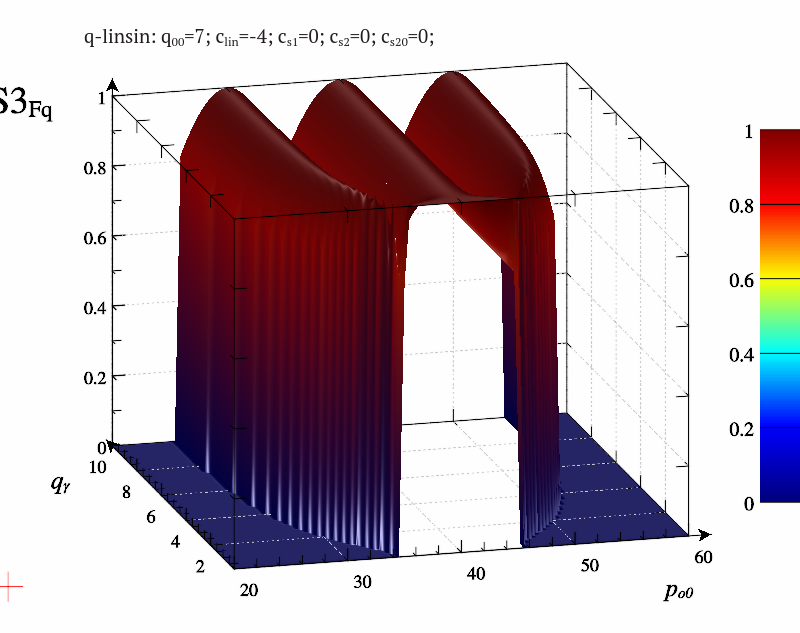
\includegraphics[width=0.32\textwidth]{p/qls_pe-p_po_qg_SFq_lin.png}
    \hfill
    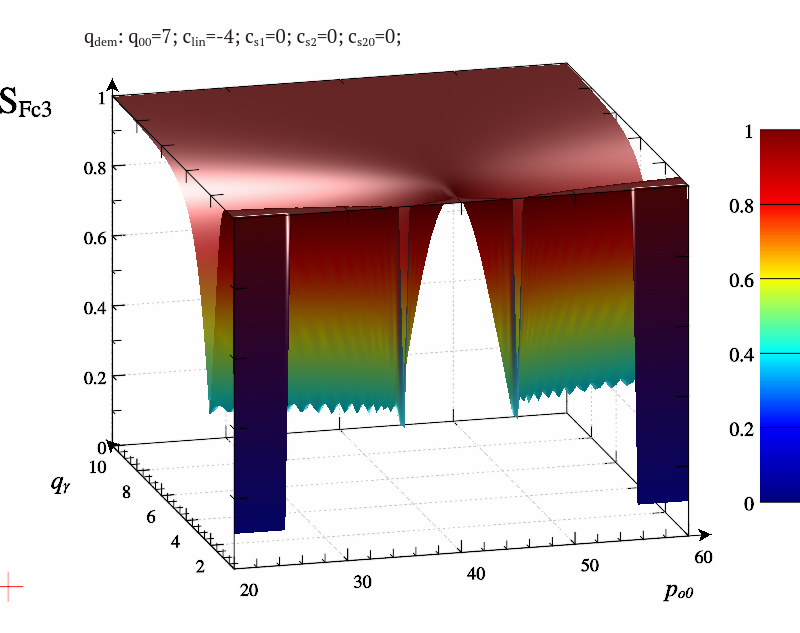
\includegraphics[width=0.32\textwidth]{p/qls_pe-p_po_qg_SFc_lin.png}
  \end{center}
  \vspace{-1.0ex}
  \begin{center}
    ~ \hfill a \hfill\hfill b \hfill\hfill c \hfill ~
  \end{center}
  \vspace{-1.5ex}
  \caption{Залежності $S(p_o,q_\gamma)$ для методів $p_{eql}$ (a), $p_{eFq}$ (b), $p_{qFc}$ (c) за умов (\ref{atu:eq:q_dem_lin})}
  \label{atu:f:qsl_S_po_qg_lin}
\end{figure}

Принципової різниці з попередніми графіками немає, так як відміни в
умовах проявляється на відносно дрібному масштабі, і не впливає
на досить грубу оцінку~$S$.

На рис.~\ref{atu:f:qsl_W_po_qg_all}, \ref{atu:f:qsl_W_po_qg_s20}, \ref{atu:f:qsl_W_po_qg_lin},
представлені залежності
$ W (p_o, q_\gamma) $ для всіх розглянутих варіантів.

\begin{figure}[htb!]
  \begin{center}
    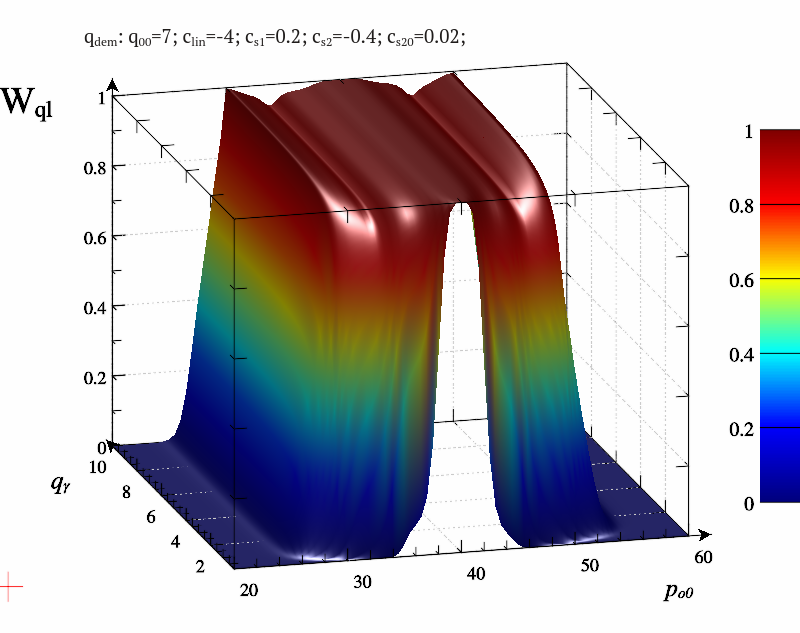
\includegraphics[width=0.32\textwidth]{p/qls_pe-p_po_qg_Wql_all.png}
    \hfill
    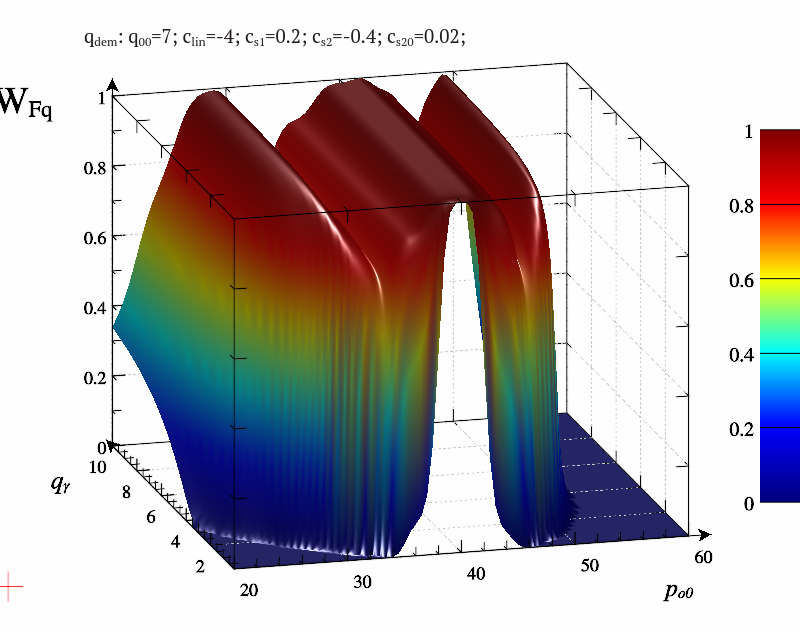
\includegraphics[width=0.32\textwidth]{p/qls_pe-p_po_qg_WFq_all.png}
    \hfill
    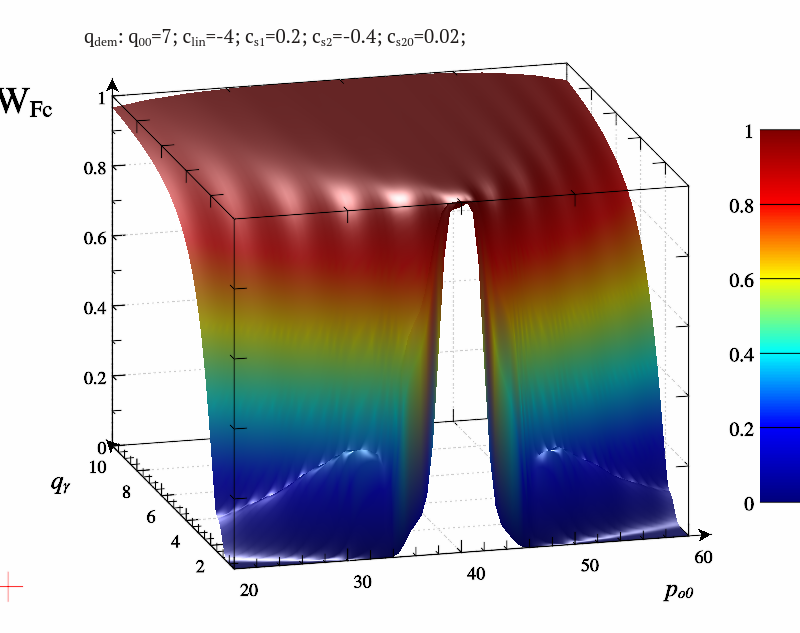
\includegraphics[width=0.32\textwidth]{p/qls_pe-p_po_qg_WFc_all.png}
  \end{center}
  \vspace{-1.0ex}
  \begin{center}
    ~ \hfill a \hfill\hfill b \hfill\hfill c \hfill ~
  \end{center}
  \vspace{-1.5ex}
  \caption{Залежності $W(p_o,q_\gamma)$ для методів $p_{eql}$ (a), $p_{eFq}$ (b), $p_{qFc}$ (c) за умов (\ref{atu:eq:q_dem_all})}
  \label{atu:f:qsl_W_po_qg_all}
\end{figure}


\begin{figure}[htb!]
  \begin{center}
    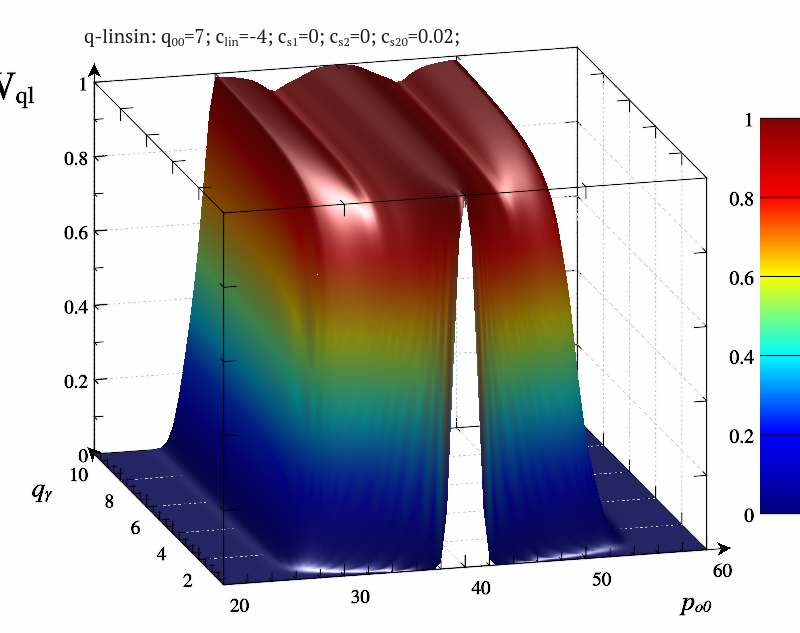
\includegraphics[width=0.32\textwidth]{p/qls_pe-p_po_qg_Wql_s20.png}
    \hfill
    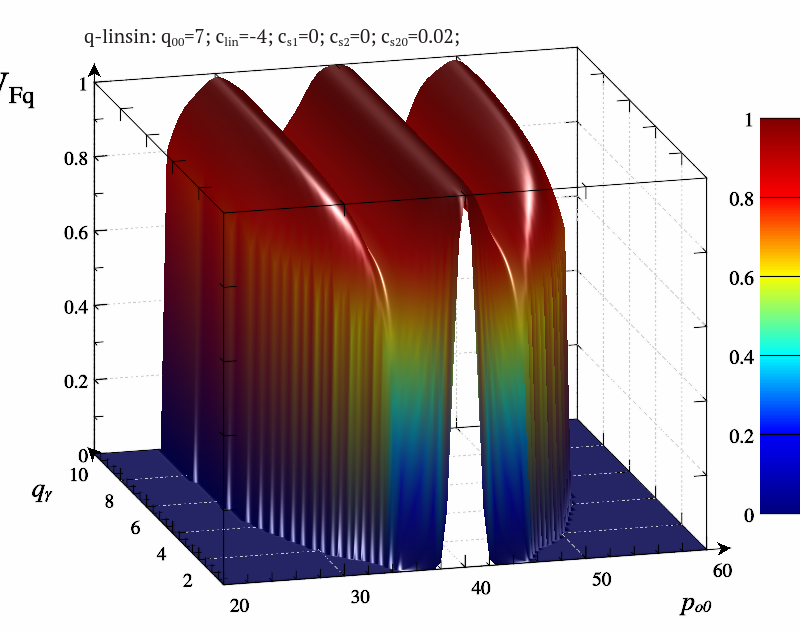
\includegraphics[width=0.32\textwidth]{p/qls_pe-p_po_qg_WFq_s20.png}
    \hfill
    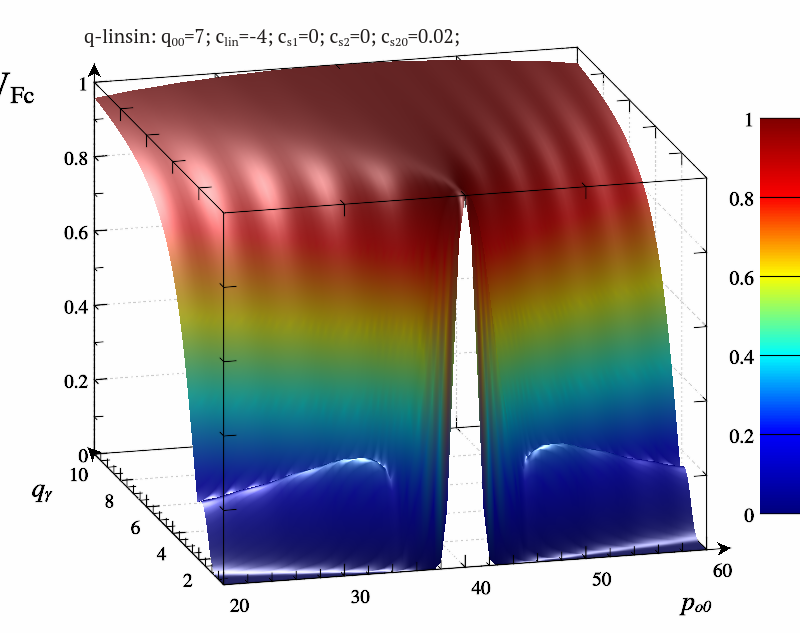
\includegraphics[width=0.32\textwidth]{p/qls_pe-p_po_qg_WFc_s20.png}
  \end{center}
  \vspace{-1.0ex}
  \begin{center}
    ~ \hfill a \hfill\hfill b \hfill\hfill c \hfill ~
  \end{center}
  \vspace{-1.5ex}
  \caption{Залежності $W(p_o,q_\gamma)$ для методів $p_{eql}$ (a), $p_{eFq}$ (b), $p_{qFc}$ (c) за умов (\ref{atu:eq:q_dem_s20})}
  \label{atu:f:qsl_W_po_qg_s20}
\end{figure}

\begin{figure}[htb!]
  \begin{center}
    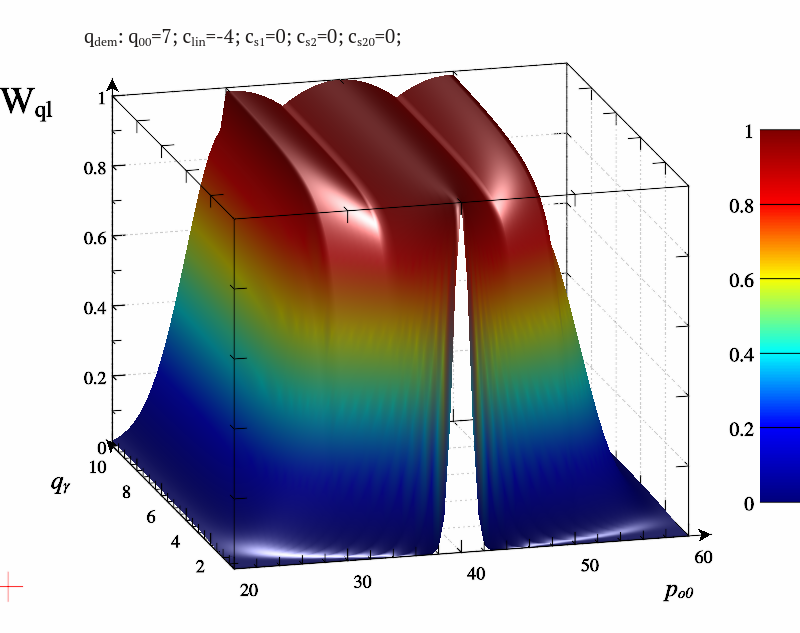
\includegraphics[width=0.32\textwidth]{p/qls_pe-p_po_qg_Wql_lin.png}
    \hfill
    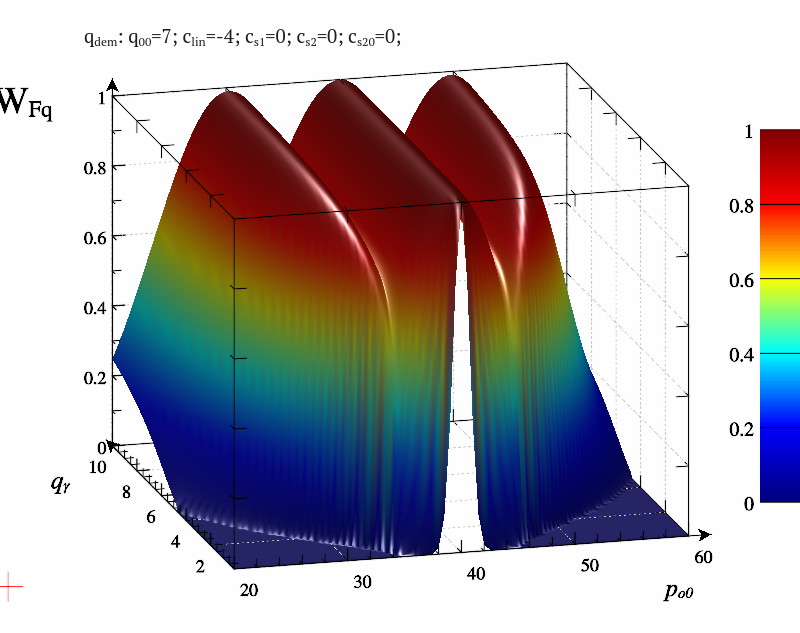
\includegraphics[width=0.32\textwidth]{p/qls_pe-p_po_qg_WFq_lin.png}
    \hfill
    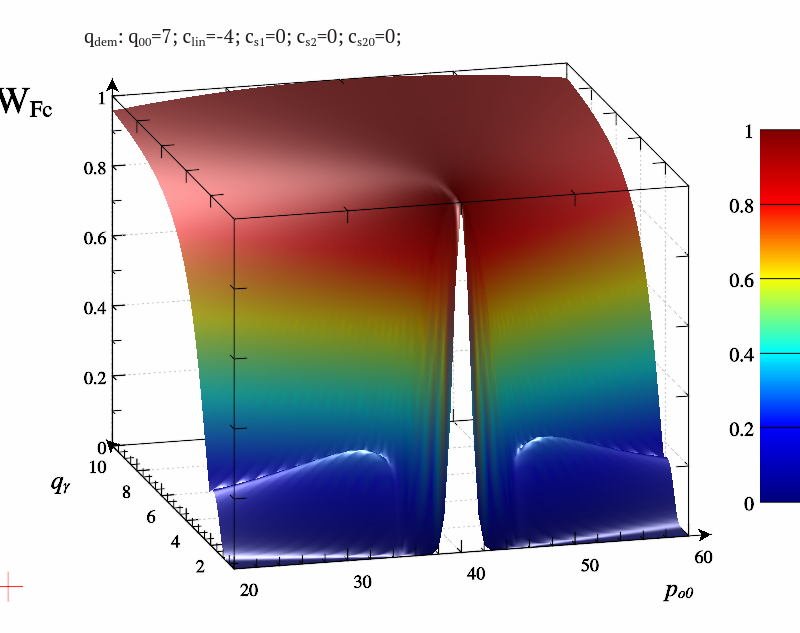
\includegraphics[width=0.32\textwidth]{p/qls_pe-p_po_qg_WFc_lin.png}
  \end{center}
  \vspace{-1.0ex}
  \begin{center}
    ~ \hfill a \hfill\hfill b \hfill\hfill c \hfill ~
  \end{center}
  \vspace{-1.5ex}
  \caption{Залежності $W(p_o,q_\gamma)$ для методів $p_{eql}$ (a), $p_{eFq}$ (b), $p_{qFc}$ (c) за умов (\ref{atu:eq:q_dem_lin})}
  \label{atu:f:qsl_W_po_qg_lin}
\end{figure}

Найбільш помітна відмінність від залежностей
$S(p_o, q_\gamma) $ спостерігається для методу
$p_{eql}$ --- починає грати роль ``штраф'' за надмірну
чутливість функції якості, яка в самому методі практично не
використовується. Однак, для розглянутої області, поблизу
робочого діапазону, відмінність
$W$ від
$S$ не має особливого значення. Основне призначення
$W$ --- обмежувати динаміку агентів, що знаходяться далеко від
шуканого значення~$p_o$.


У другій серії обчислювальних експериментів значення параметра об'єкта було
фіксованим $p_o = 39$, а відстань між агентами $A$ змінювалося від $0.1$
до $20$. При цьому, при $A <1$ точка $p_o$ перебувала за межами інтервалу
$[p_l, p_r]$, і положення $p_e$ визначалося за допомогою екстраполяції.
Значна частина цих графіків відображає протилежний випадок --- $p_O \in [p_l,p_r]$,
і значення $p_e$ визначається інтерполяцією на розширенні (з ростом $A$) діапазоні.

На рис.~\ref{atu:f:qsl_pe_A_qg_all} подані поверхні залежностей помилок ідентифікації
при наявності всіх нелінійних членів.


\begin{figure}[htb!]
  \begin{center}
    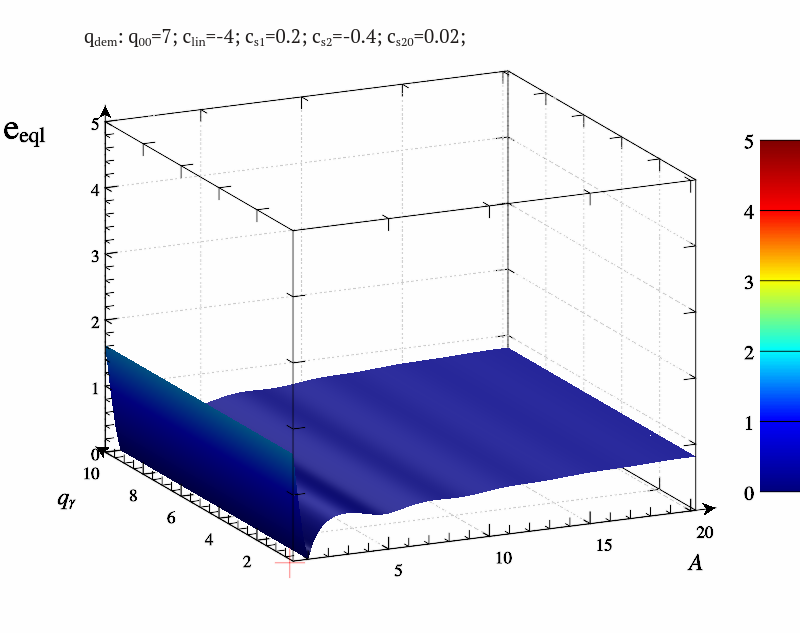
\includegraphics[width=0.32\textwidth]{p/qls_pe-p_A_qg_eql_all.png}
    \hfill
    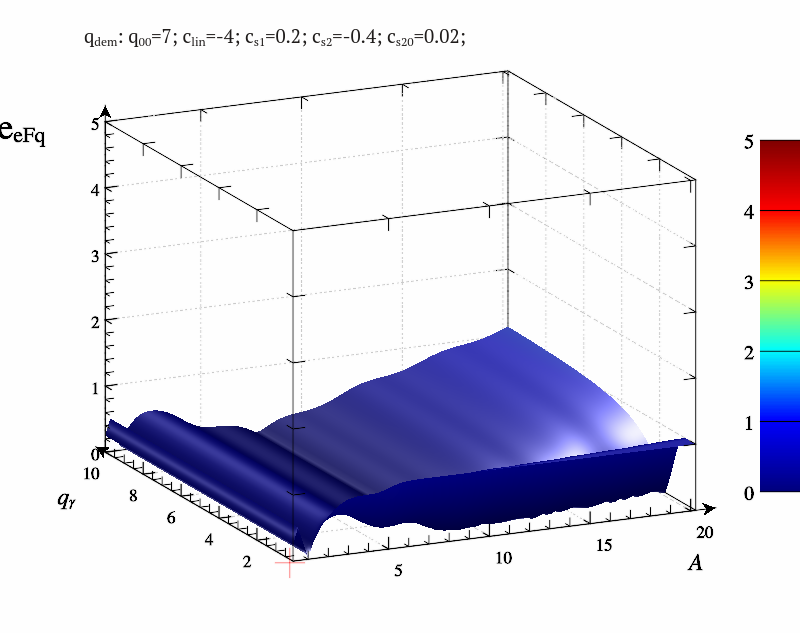
\includegraphics[width=0.32\textwidth]{p/qls_pe-p_A_qg_eFq_all.png}
    \hfill
    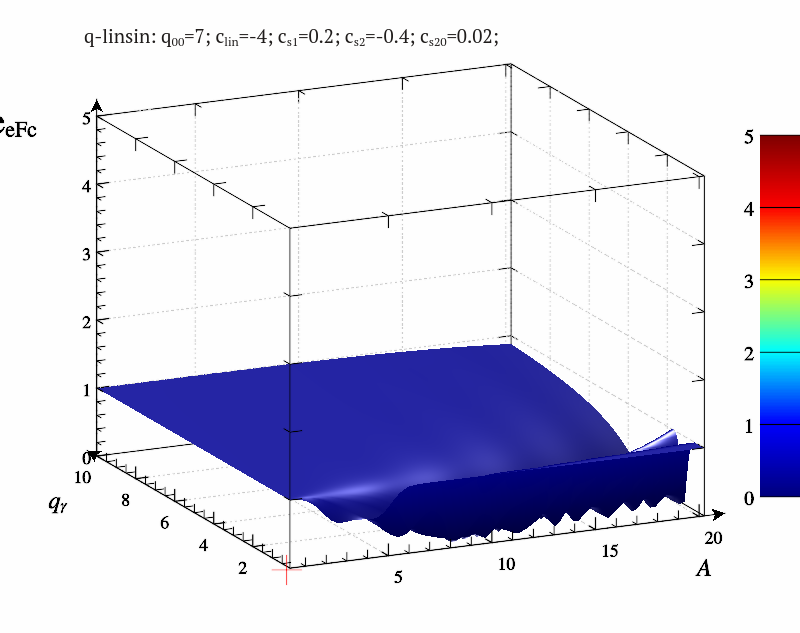
\includegraphics[width=0.32\textwidth]{p/qls_pe-p_A_qg_eFc_all.png}
  \end{center}
  \vspace{-1.0ex}
  \begin{center}
    ~ \hfill a \hfill\hfill b \hfill\hfill c \hfill ~
  \end{center}
  \vspace{-1.5ex}
  \caption{Залежності $e(A,q_\gamma)$ для методів $p_{eql}$ (a), $p_{eFq}$ (b), $p_{qFc}$ (c) за умов (\ref{atu:eq:q_dem_all})}
  \label{atu:f:qsl_pe_A_qg_all}
\end{figure}

Для методу $p_{eql}$ форма цього графіка досить передбачувана --- немає
залежності від $q_\gamma$, на ділянці екстраполяції величина похибки
лінійно падає при $A \to p_c - p_o$. При подальшому зростанні $A$ похибка
помірно зростає, причому в цьому зростанні можна виділити дві ділянки. Перша
характеризується відносно різким зростанням похибки, що пов'язано зі збільшенням
впливу високочастотних нелінійних членів, друга --- досить плавним підйомом.

Графік, відповідний методу $p_{eFq}$ виявляє явну залежність похибки від
$q_\gamma$. Для широкого діапазону величини $ A $ існує досить вузька область
значень $q_\gamma$, при яких похибка мінімальна. Як надмірна, так і
недостатня чутливість функції якості призводить до зростання похибки.

На жаль, навіть для найпростіших випадків, подібних розглядався,
отримання аналітичної залежності у цій галузі утруднено. Також
цей графік відрізняється меншою похибкою в режимі
екстраполяції, але в цілому цей метод програє попередньому.

Графік похибки для методу $p_{eFc}$ підкреслює обмежену придатність цього методу.
Аналогічно до попереднього методу, існує область найбільш
сприятливих для проведення ідентифікації значень
$ q_\gamma $. Однак, рівень похибки практично не падає при
$ p_l \to p_o $, тобто цей метод не виграє в точності при концентрації
агентів в околі
$ p_o $.

Графіки (рис.~\ref{atu:f:qsl_pe_A_qg_s20}), побудовані з використанням тільки
високочастотних нелінійних членів, підтверджують викладені
вище припущення про вплив нелінійностей різного частотного
масштабу на похибку ідентифікації.

\begin{figure}[htb!]
  \begin{center}
    \includegraphics[width=0.32\textwidth]{p/qls_pe-p_A_qg_eql_s20.png}
    \hfill
    \includegraphics[width=0.32\textwidth]{p/qls_pe-p_A_qg_eFq_s20.png}
    \hfill
    \includegraphics[width=0.32\textwidth]{p/qls_pe-p_A_qg_eFc_s20.png}
  \end{center}
  \caption{Залежності $e(A,q_\gamma)$ для методів $p_{eql}$, $p_{eFq}$, $p_{qFc}$ за умов (\ref{atu:eq:q_dem_s20})}
  \label{atu:f:qsl_pe_A_qg_s20}
\end{figure}

При цьому метод
$ p_{eql} $ характеризується практичною відсутністю зростання
похибки як в режимі екстраполяції, так і при значному зростанні
$ A $. Метод
$ p_{eFq} $ також характеризується істотно меншим зростанням
похибки, за винятком області надмірної чутливості. Вид графіка
для методу
$ p_{eFc} $ практично не змінився.

В ідеальному випадку, при лінійної залежності
$ q_\mathrm{dem} (p) $~(рис.~\ref{atu:f:qsl_pe_A_qg_lin}), метод
$ p_{eql} $ демонструє ідеальні результати. Слід зазначити, що в
даній тестовій задачі відсутні похибки вимірювання.

Метод
$ p_{eFq} $ дозволяє досягти малою, але не нульовий
похибки всюди, за винятком області екстраполяції і підвищеної
чутливості. При цьому, рівень помилок навіть у несприятливих
областях відносно малий. Навпаки, метод
$ p_{eFc} $, навіть в ідеальних умовах продовжує показувати тільки задовільні
результати.

\begin{figure}[htb!]
  \begin{center}
    \includegraphics[width=0.32\textwidth]{p/qls_pe-p_A_qg_eql_lin.png}
    \hfill
    \includegraphics[width=0.32\textwidth]{p/qls_pe-p_A_qg_eFq_lin.png}
    \hfill
    \includegraphics[width=0.32\textwidth]{p/qls_pe-p_A_qg_eFc_lin.png}
  \end{center}
  \caption{Залежності $e(A,q_\gamma)$ для методів $p_{eql}$, $p_{eFq}$, $p_{qFc}$ за умов (\ref{atu:eq:q_dem_lin})}
  \label{atu:f:qsl_pe_A_qg_lin}
\end{figure}

Таким чином, на підставі результатів моделювання можна зробити висновки про
можливість застосування розглянутих методів:


\begin{itemize}

  \item
    Метод $p_{eFc}$ має гранично  обмежену придатність,
    єдині переваги --- простота реалізації,
    відсутність особливих випадків і природна обмеженість
    $ p_e $ не повністю компенсують недоліки, тому в подальших
    дослідженнях в даній цей метод застосовуватися не буде.

  \item
    При нормальному функціонуванні метод $p_{eql}$ забезпечує найкращі
    результати. При цьому він складніше у реалізації, вимагає обробки ряду
    особливих випадків.

  \item
    Метод $p_{eFq}$ демонструє результати, які можна
    порівняти з методом $p_{eql}$, при цьому він простіший у реалізації. У тих
    випадках, коли величина критерію самому агенту безпосередньо не відома, цей
    метод, на відміну від методів, заснованих на апроксимації $q (p)$, зберігає
    працездатність. Недоліком є істотна залежність від величини $q_\gamma$.

    Проте, навіть методи, які не використовують функцію якості на
    рівні агента, все одно застосовують її на рівні координатора
    пошуку, і завдання вибору адекватної величини
    $ q_\gamma $ все одно залишається.

  \item
    Методи $p_{eql}$ і $p_{qFq}$ дозволяють досягти меншої похибки
    ідентифікації при зближенні пошукових агентів до $p_o$, за умови $p_o \in [p_l, p_r]$.
    Отже, для підвищення точності ідентифікації необхідно або
    реалізовувати пошукову динаміку об'єкта, або ж нарощувати
    кількість нерухомих агентів, що може бути недосяжно в умовах
    обмеженості ресурсів.


\end{itemize}




% }}}2

\subsection{Динаміка пошукових агентів}%{{{2

Значення $p_e$, отримане пошуковим агентом, може використовуватися
безпосередньо і миттєво в якості значення параметрів для керованих моделей
тільки в тому випадку, якщо об'єкт, і отже моделі, не виявляють власної
динаміки, тобто є статичними. Ідентифікація статичних об'єктів не є ціллю
цієї роботи.

При моделюванні довільної нелінійної динамічної системи,
а особливо хаотичних систем, немає можливості строго
визначити допустиму динаміку зміни параметрів в процесі
ідентифікації. Більш того, існують навіть лінійні системи, для
яких малі, але спеціальним чином підібрані параметричні впливу
призводять до необмеженого росту значень, що відображають
стан системи. Одним з найвідоміших прикладів такої поведінки є
параметричний резонанс~\cite{landau1}. Для систем динамічного хаосу
більш відомим явищем є сигнальна синхронізація систем, однак,
можливість аналогічних параметричних впливів досить очевидна.

Проте, якщо виключити досить рідкісні особливі випадки, можна
оцінити допустиму динаміку зміни параметрів. Перш за все,
в процесі синтезу критерію ідентифікації одним з етапів є
визначення коректного значення
$\tau_q$ (або $a_q$).
Найчастіше, ця величина неявно задає і допустиму
швидкість зміни параметрів моделей в процесі ідентифікації.

При моделюванні динаміки тіла без урахування обертання в механіці досить задати
всі сили, що діють на це тіло. Аналогічно, визначаючи пошукову динаміку агента
потрібно визначити еквівалент ``сил'', що викликають зсув параметрів моделей,
контрольованих агентом. При цьому задачу визначення динаміки можна спростити,
розділивши ``сили'' на дві групи. До першої входять сили, що призводять до ``руху''.
У другу входять сили опору, і, замість розгляду самих сил, досить
визначити правила динаміки, при цьому можливе використання правил, які не мають
прямого відображення на реальні фізичні системи.
Такий поділ дозволяє дозволяє більш простим чином класифікувати
способи завдання пошукової динаміки.


\subsubsection{Визначення сил, що використовуються при описі динаміки пошукового агента} % {{{3

Розглянемо способи визначення основних діючих сил.

$f_e$ ---
``сила тяжіння'' до локальної оцінки $p_e$, забезпечує зміщення
агента в напрямку цієї точки, і, отже, збільшення ``щільності'' агентів в
околі $p_o$.
Розглянемо можливі способи визначення.

Найпростішим, очевидним, з прозорим фізичним змістом є
наступне визначення:
%
\begin{equation}
  f_e(t) = - k_e \left( p_c(t) - p_e(t) \right)  ,
  \label{atu:eq:f_e_lin}
\end{equation}
%
де $k_e$ --- коефіцієнт пропорційності, що відповідає коефіцієнту жорсткості
умовної ``пружини'', що деформується при видаленні $p_c$ від $p_e$. Це
визначення досить універсальне і має сенс при реалізації багатьох пошукових
тактик.
%
Проте, це визначення не позбавлене недоліків. Перш за все,
потенційна яма, яка формується силою виду~(\ref{atu:eq:f_e_lin}), має параболічну
форму, і якщо агент знаходиться на дні цієї ями, малі зовнішні
сили легко виводять агента з центру даної ями, що, в свою чергу,
може призводити до зниження точності ідентифікації.

Вищезгаданого недоліку позбавлене наступне визначення:
%
\begin{equation}
  f_e(t) = - k_e \sign \left( p_c(t) - p_e(t) \right) ,
  \label{atu:eq:f_e_sign}
\end{equation}
%
при цьому сила утворює трикутну потенційну яму.
Але, усунення одного
недоліку призводить до появи декількох інших. Перш за все,
наявність розриву цієї функції вимагає прийняття спеціальних
заходів щодо забезпечення обчислювальної стійкості алгоритмів
при чисельному моделюванні. З іншого боку, постійне значення
цієї функції при віддаленні
$ p_c $ від
$ p_e $ може привести до зниження швидкості пошуку. В першу чергу
до цього недоліку будуть схильні методи ідентифікації з одним
агентом.

Проміжний спосіб визначення розглянутої ``сили'' дає наступне
визначення:
%
\begin{equation}
  f_e(t)
  = - k_e \cdot
  \begin{cases}
    1 &  p_c(t) - p_e(t)  > p_\mathrm{sat}
    \\
    \frac{p_c(t)-p_e(t)}{p_\mathrm{sat}} & | p_c(t)-p_e(t)| \le p_\mathrm{sat}
    \\
    -1 &  p_c(t) - p_e(t)  < -p_\mathrm{sat}
  \end{cases},
  \label{atu:eq:f_e_sat}
\end{equation}
%
де  $p_\mathrm{sat}$ ---
мала в порівнянні з областю пошуку величина. Це визначення в
якійсь мірі поєднує переваги і недоліки двох попередніх. Немає
розриву в нулі, малі зовнішні обурення призводять до досить
обмеженим зсувів, але обмеженість цієї залежності, як і
попередньої, робить незручним використання цього визначення
для систем з одним агентом.

Загальним недоліком визначення сили $f_e$ за виразом (\ref{atu:eq:f_e_lin})
є той факт, що сила визначається тільки по локальним параметрами в околі
агента. Більш того, ігнорується навіть локальне значення впевненості агента в
оцінці $p_e$.

Для агентів, що знаходяться в безпосередній близькості до
$ p_o $, таке визначення сили виправдано. Всі інші агенти в разі
правильного визначення напрямку, будуть цією силою притискатися
до краю своєї смуги, якщо вона є, або ж виявляти тенденцію до
сильного скупчування в іншому випадку. Більш того, для агентів,
що знаходяться далеко від шуканого значення, вплив помилок
вимірювання призводить до постійної зміни оцінки напрямки до
$ p_o $, і як наслідок --- до сильного ``рисканню'' таких агентів. Отже,
необхідне обмеження цієї сили, на підставі локальних,
глобальних, або ж і тих і інших оцінок. наприклад:
%
\begin{equation}
  f_e(t) = - k_e S(t) \left( p_c(t) - p_e(t) \right) ,
  \label{atu:eq:f_e_lin_S}
\end{equation}
%
\begin{equation}
  f_e(t) = - k_e F_c(t) \left( p_c(t) - p_e(t) \right) ,
  \label{atu:eq:f_e_lin_F}
\end{equation}
%
\begin{equation}
  f_e(t) = - k_e W(t) \left( p_c(t) - p_e(t) \right) ,
  \label{atu:eq:f_e_lin_W}
\end{equation}


Наявність тільки сили $f_e$ призводить до того, що поведінка агентів буде
практично незалежною, і для реалізації властивостей ``ансамблю'' агентів
необхідне введення сил, що регламентують колективну поведінку. В першу чергу,
слід визначити силу $f_n$, яка визначає взаємодію агента з найближчими
сусідами. У досить загальному випадку цю силу можна визначити як
%
\begin{equation}
  f_n( p_r, p_c, p_l ) = f_{nr}(p_r-p_c) + f_{nl}(p_c-p_l).
  \label{atu:eq:f_n_gen}
\end{equation}

У разі лінійності і однакових визначень функцій $f_{nr}$ і $f_{nl}$ ця залежність набуває вигляду
%
\begin{equation}
  f_n = k_n ( p_r - 2 p_c + p_l ),
  \label{atu:eq:f_n_lin}
\end{equation}
%
де $k_n$ --- масштабний коефіцієнт, що відповідає коефіцієнту жорсткості
``пружин'', що з'єднують агентів. При цьому слід зазначити, що ця функція буде
приймати нульові значення при будь-якому рівномірному розподілі агентів.
І, відповідно, буде протидіяти впливам, що призводять до
нерівномірного розподілу. При цьому немає поняття ``природної відстані''
між об'єктами, на якому вони знаходяться в стані стійкої рівноваги при
$ f_e = 0 $.

При певних співвідношеннях між
$ k_e $ і
$ k_n $ можлива ситуація, коли траєкторії двох агентів
перетинаються. Для деяких типів агентів, наприклад
$ p_{eFc} $ це не викликає особливих проблем. Для більшості інших
наявність таких перетинів є випадком, коли методи визначення
$p_e$ дають принципово невірні, в тому числі невизначені
результати. Одним із способів недопущення подібних станів є
призначення агентам робочих діапазонів (``смуг''), які не перетинаються.

Другим --- використання нелінійної функції $f_n$,
яка забезпечую сильне, навіть нескінченне відтискування
агентів при зближенні, наприклад:
%
\begin{equation}
  f_n = k_n \left( \log\left( \frac{p_r-p_c}{p_{d0}} \right) -  \log\left( \frac{p_c-p_l}{p_{d0}}\right) \right),
  \label{atu:eq:f_n_log}
\end{equation}
%
де
$p_{d0}$ ---
базова відстань між агентами, що зазвичай дорівнює початкової відстані:
$p_{d0} = \frac{\Delta p}{N-1}$.




Наявність функції
$ f_n $ забезпечує певні аспекти колективної поведінки агентів,
протидіючи невиправданої скупченості агентів. Тем не менше,
наявності цієї функції в багатьох задачах недостатньо для
побудови працездатної системи ідентифікації. В першу чергу,
базовий вид цієї функції не перешкоджає рівномірному стиску
або розтягу, протидію викликає лише нерівномірність цих
процесів. Більш того, ``пилкоподібна'' залежність параметра
об'єкта від часу може призводити до ситуації, коли значення
параметра агента відстежуватимуть послідовно різні агенти, і
як наслідок, весь ансамбль агентів буде послідовно зміщуватися
в одну сторону. Таким чином, потрібна як мінімум ще одна сила,
яка буде перешкоджати таким небажаним ефектам.

Має сенс використовувати $f_c$ --- ``силу тяжіння'' до початкового значення параметра
($p_{c}(0)$) для даної моделі. У лінійній постановці ця сила визначається як
%
\begin{equation}
  f_c = -k_c (p_c - p_{c}(0)) ,
  \label{atu:eq:f_c}
\end{equation}
%
де $k_c$ --- коефіцієнт, що відповідає жорсткості ``пружини'',
що зв'язує агента з його початковим положенням.
Добре зарекомендували себе як нелінійні ``бар'єри'',
так і алгоритмічні методи, які утримують агента
більш-менш жорстко у виділеному йому діапазоні параметра.

Існування сил
$f_n$ і $f_c$
не дає всім моделям прийняти одне і те ж значення параметра
поблизу екстремуму, і, отже, припинити процес пошуку. Це також
дозволяє швидко переключитися на іншу модель в разі швидкої
зміни параметра об'єкта.

Результати моделювання показали, що в може мати
сенс введення додаткових сил ``бар'єрного'' виду, для виключення
перетину траєкторій пошукових агентів, або ж їх відходу з
робочого діапазону.

Системи ідентифікації з одним агентом не вимагають опису
динаміки колективної поведінки, і для них сили
$ f_n $ і
$ f_c $ розумно вважати нульовими. Проте, в цьому випадку постановка
задачі може вимагати обмеження значень параметра моделі. Цього
можна досягти як введенням додаткових функцій ``бар'єрного ''
виду на границі області, так і алгоритмічними обмеженнями.

Зважаючи на вищезазначене, визначимо суму всіх ``сил'',
що діють на пошукового агента:
\begin{equation}
  f_t = f_c + f_n + f_e .
  \label{atu:eq:f_t}
\end{equation}



% }}}3



\subsubsection{Способи визначення пошукової динаміки агента при заданій силі}  % {{{3

\paragraph{Метод ``важкої кульки''}

У цьому випадку пошукова динамка задається наступним чином:
%
\begin{equation}
  m \ddot{p}_c + \nu \dot{p}_c = f_t(t),
  \label{atu:eq:heavy_ball}
\end{equation}
%
де $m$ --- еквівалент маси кульки, $\nu$ --- коефіцієнт умовної в'язкості.
%
Застосування цього підходу виправдано, в першу чергу, при
використанні системи ідентифікації з одним пошуковим агентом. В
цьому випадку послаблюються вимоги на монотонність залежності
$q(p)$, або ж існування лише одного екстремуму
$F(p)$. До недоліків даного підходу слід віднести відносно великі
обчислювальні витрати, і підвищені вимоги до стійкості пошуку.


\paragraph{Метод ``динаміки тіла у в'язкій рідині''}

Також може використовуватися наближення динаміки тіла у в'язкій рідині, коли
вплив інерції дуже малий в порівнянні з в'язкістю, при цьому зміни параметрів
моделей (пошукових агентів) задаються наступним чином:
%
\begin{equation}
  \od{p_c}{t} = v_f f_t(t),
  \label{atu:eq:v_f}
\end{equation}
%
\noindent
де $f_t$ --- сума всіх діючих ``сил'',
$v_f = 1 / \nu$ --- коефіцієнт
пропорційності. Даний підхід, в порівнянні з попереднім, вимагає менших
обчислювальних витрат, і проявляє більшу стійкість. Більш слабкі пошукові
здібності компенсуються застосуванням множини агентів. Тому, в подальшому
викладі для багатомодельних систем буде застосовуватись саме цей підхід.

\paragraph{Спеціальні підходи}

Існують методи адаптивно-пошукової ідентифікації, що визначають
свої правила опису пошукової динаміки. При цьому, можуть не
вводиться поняття
$ p_e $,
$ f_t $ і інші. Проте, в цілому, ці спеціальні способи визначення
динаміки можна звести до використовуваної термінології.

Так, наприклад, оригінальний адаптивно-пошуковий метод
використовує пошукові коливання і для визначення швидкості
зсуву, і для реалізації зміщення як такого. При цьому, після
усереднення на інтервалі пошукового періоду, динаміка пошуку
може бути описана виразом~(\ref{atu:eq:v_f}).

Метод з двома моделями і двома КГПК також задає пошукову
динаміку спеціальним чином. На відміну від попереднього випадку,
для визначення швидкості зсуву параметрів використовується
пара моделей, і зміщення реалізується за рахунок різниці
спрацьовування двох КГПК. Проте, і в цьоиу разі, після усереднення,
динаміка може бути описана виразом~(\ref{atu:eq:v_f}).


% }}}3


% }}}2



% }}}1

\section{Методи, параметри і алгоритми роботи пошукових координаторів} % {{{1

\subsection{Методи визначення значення ідентифікованого параметра координатором пошуку} % {{{2


Розглянемо набір підходів визначення пошуковим координатором точки максимуму
функції якості, а отже --- значення ідентифікованого
параметра~\cite{atu_st99,atu_jacs2015,atu_st103}.


З усього списку вихідних сигналів пошукових агентів координатор використовує
тільки необхідну йому підмножину.
У будь-якому випадку, йому необхідні координати агентів в
просторі параметрів, а також величини, що визначають рівень
важливості даних даного агента для визначення
$ p_\mathrm{id} $.
У якості координати може використовуватися як $p_c$, так і $p_e$.
У якості рівня важливості може використовуватися $F$, $S$, $W$.
Можливі й більш складні методи, які використовують більшу
кількість вихідних сигналів агента.

В якості першого наближення $p_\mathrm{id}$ можна  використовувати
значення $p_c$ тієї моделі, для якої функція якості максимальна:
%
\begin{equation}
  p_{bcF}
  =
  p_{c,i};
  \quad
  i : F_i = \max{F_j}, \, j=0 \ldots N-1 .
  \label{atu:eq:p_bcF}
\end{equation}

Аналогічно визначаються залежності
$p_{bcS}$ та $p_{bcW}$.
%
Застосування величини
$ p_{bcS} $ здається досить сумнівною, оскільки величина
$S$ визначається кожним агентом тільки на підставі локальних
даних, і агенти можуть бути повністю ``впевнені'' в своїй оцінці
$ p_o $, навіть в тому випадку, якщо вони знаходяться досить далеко
від значення
$ F \approx 1 $, але за рахунок перешкод вимінювання отримали цілком
правдоподібну апроксимацію
$ q (p) $ або
$ F (p) $.

Єдиною перевагою даного методу є простота реалізації. При цьому, ніяк не
використовуються апроксимуючи здатності агентів. Більш того, залежності
$p_{bcA}(t)$ схильні до стрибкоподібних змін в момент перемикання з однієї моделі
на іншу.

Слід зазначити, що для методів, які використовують одну модель, це
практично єдиний метод визначення
$p_\mathrm{id}(t)$.

Для того, щоб використовувати апроксимуючи можливості кожного агента у
визначенні (\ref{atu:eq:p_bcF}) замість $p_c$ можна використовувати $ p_e$.
Відповідні методи отримають позначення $p_{beS}$, $p_{beS} $ і $p_{beW}$.

Такі визначення, на відміну від (\ref{atu:eq:p_bcF}), дозволяють,
при досить хорошій апроксимації $q(p)$ принаймні одним кращим агентом,
реалізувати ідентифікацію для будь-якого
$p_o \in [p_{\min}, p_{\max}]$ при нерухомих агентах.

Природно, при цьому точність ідентифікації буде падати, особливо
при вираженій нелінійності
$ q (p) $, але значення
$ p_\mathrm{id} $ не будуть обмеженим набором точок~$p_{i,0}$.
При цьому слід зазначити, що значення
$p_e$ параметра не відповідає жодної моделі, отже, значення як
функції якості
$F$, так і похідною від неї величини
$W$ для цієї точки невідомо. Для тих методів оцінки
$p_e$, які дозволяють апроксимувати значення
$F_e$, надійність цієї оцінки може бути сумнівна. Проте, похибки,
що виникають при такій заміні, повинні мінімізуватися в процесі
пошуку при
$ p_{e, i} \to p_o $.


Наступний метод --- реалізація методу
COG (Center of gravity, Такагі-Сугено)~\cite{atu_asau25,atu_csit2015,atu_asau16},
який використовується при дефазифікації систем нечіткої логіки для всього
ансамблю:
%
\begin{equation}
  p_{gcF}
  =
  \frac{\sum\limits_{i=0}^{N-1} F_{i} p_{ci}}
       {\sum\limits_{i=0}^{N-1} F_{i} }
  .
  \label{atu:eq:p_gcF}
\end{equation}

Аналогічно визначаються методи
$p_{gcS}$,
$p_{gcW}$,
$p_{geF}$,
$p_{geS}$ та
$p_{geW}$.


Наступний підхід має призначення зменшити залежність попереднього від впливу локальних
екстремумів і границь. В цьому випадку визначається модель $M_{i_{m}}$ ($M_{c}$) з
максимальним значенням $F$, а в оцінці використовується тільки найближчий
окіл цієї моделі:
%
\begin{equation}
  p_{lcF}
  =
  \frac{ F_{i-1} p_{c,i-1} + F_{i} p_{c,i} + F_{i+1} p_{c,i+1} }
       { F_{i-1}           + F_{i}         + F_{i+1}         }
  ;
  \quad
  i : F_i = \max{F_j}, \, j=0 \ldots N-1 .
  \label{atu:eq:p_lcF}
\end{equation}
%
або, з урахуванням введених локальних позначень при $ i = c $:
%
\begin{equation}
  p_{leF}
  =
  \frac{ F_{l} p_{l} + F_{c} p_{c} + F_{r} p_{r} }
       { F_{l}       + F_{c}       + F_{r}       }
  .
  \label{atu:eq:p_lcFl}
\end{equation}

Аналогічно визначаються методи
$p_{lcS}$,
$p_{lcW}$,
$p_{leF}$,
$p_{leS}$ та
$p_{leW}$.

Так само в околі кращого агента можна використовувати інтерполяцію по
$F$, аналогічно (\ref{atu:eq:p_eFq}). В позначенні таких методів будемо
використовувати перший символ ``q'', наприклад $p_{qeF}$.


Похибки ідентифікації в просторі параметрів для розглянутих підходів позначимо відповідно:
%
\begin{equation}
  e_{gcF} = p_{gcF} - p_o,
  \quad
  e_{leF} = p_{leF} - p_o,
  \quad
  \ldots
  \quad
  e_{leW} = p_{leW} - p_o.
  \label{atu:eq:e_xx}
\end{equation}
%
Якщо немає необхідності вказувати конкретно
$ F $,
$ S $ або
$ W $, то останній символ в індексі будемо опускати, або замінювати на~``A''.



% }}}2


% }}}1


\section{Класифікація і позначення систем ідентифікації}%{{{1
\label{atu:id_classification}

У даній роботі розглядається набір методів ідентифікації нелінійних динамічних
систем. При цьому, більшість з них мають загальні властивості, і система
ідентифікації в цілому складається з ``набору'' модулів і алгоритмів,
комбінація яких дозволяє вибрати конкретний метод, що підходить для даної
задачі.

Отже, виникає питання коректного і несуперечливого позначення
використовуваного методу. Зважаючи на значну кількість методів,
отриманих шляхом комбінації їх елементів, не має сенсу давати
кожному окреме назви. Виникає потреба в уніфікації позначень
методів, і відповідно, введення певної класифікації. Окремі елементи
класифікації вже використовувалася при визначенні методів
роботи агентів і пошукових координаторів.

Пропонується до використання наступна система позначень, яка послідовно визначає
компоненти системи ідентифікації, починаючи з агентів.

\begin{enumerate}

  \item
    Перший символ (``F'', ``q'', ``x'') визначає,
    яка величина використовується кожним агентом для визначення $p_e$.

    Для позначення методів, для яких в якості критерію
    використовується безпосередньо виходи моделей і об'єктів, буде
    використовуватися символ ``x''. При необхідності, при появі нових
    підходів, можуть бути призначені додаткові символи.

  \item
    Другий символ
    задає спосіб визначення величини $p_e$ одним агентом.

    \begin{description}

      \item[l]  --- ``linear'' ---
        використовується лінійна апроксимація, можливо кусочно-лінійна;

      \item[q]  --- ``quadratic'' ---
        використовується апроксимація другого порядку;

      \item[с] --- ``COG'' ---
        метод ``Center of Gravity'' по околу агента;

      \item[i] --- ``implicit'' ---
       $ p_e $ не задається, динаміка агента задається в неявному вигляді;

      \item[s] --- ``special'' ---
        спосіб визначення обраний на підставі особливих апріорних
        відомостей про вид залежності~$q(p)$;

    \end{description}

  \item
    Третій символ визначає локальну пошукову геометрію, найчастіше --- кількість
    агентів в в пошуковій групі, наприклад: ``2'' --- пошукова пара, ``3'' --- триплет.
    При застосуванні методів, які використовують тільки один
    пошуковий агент, цей елемент класифікації вказує кількість
    моделей, керованих цим агентом.

  \item
    Четвертий символ
    описує поведінку додаткових моделей, які розташовані на границі:
    \begin{description}

      \item[z]  --- ``zero'' ---
        реальна модель не використовується, функція якості
        $ F $ для неї вважається нульовою;

      \item[r] --- ``real'' ---
        використовується реальна модель, але без можливості її зсуву;

      \item[а] --- ``approximate'' ---
        значення критерію і функції якості якимось чином
        апроксимуюся;

      \item[n] --- ``none'' ---
        додаткові моделі не використовуються;

    \end{description}

  \item
    П'ятий символ
    позначає обрану залежність для величини $f_e$ (або
    аналогічної величини, якщо $f_e$ безпосередньо не використовується):
    \begin{description}

      \item[c]  --- ``const'' ---
        величина $f_e $ не бере участі в описі динаміки пошукового агента;

      \item[l] --- ``linear'' ---
        величина $ f_e $ лінійно залежить від $ p_e $~(\ref{atu:eq:f_e_lin});

      \item[s] --- ``sign'' ---
        використовується залежність виду~(\ref{atu:eq:f_e_sign});

      \item[u] --- ``saturate'' ---
        використовується залежність виду~(\ref{atu:eq:f_e_sat});

    \end{description}

  \item
    Шостий символ  визначає множник,
    що використовується для величини $f_e$ при визначенні динаміки об'єкта:
    \begin{description}

      \item[o]  --- ``one'' ---
        додатковий множник не використовується (=1);

      \item[F] ---
        використовується значення функції якості;

      \item[S] ---
        використовується значення ``впевненості'' агента;

      \item[W] ---
        використовується значення ``гідності''.

    \end{description}

  \item
    Сьомий символ
    вказує, яким чином величина $f_t$ (або її еквівалент) впливає на динаміку агента:
    \begin{description}

      \item[z]  --- ``zero'' ---
        агент нерухомий;

      \item[v] --- ``viscous'' ---
        використовується модель в'язкої динаміки~(\ref{atu:eq:v_f});

      \item[b] --- ``ball'' ---
        використовується підхід ``важкої кульки''~(\ref{atu:eq:heavy_ball});

      \item[s] --- ``special'' ---
        особливий вид, задається методом безпосередньо.

    \end{description}

  \item
    Восьмий символ дозволяє вказати,
    який додатковий пошуковий рух реалізує агент:
    \begin{description}

      \item[n]  --- ``none'' ---
        додаткове пошуковий рух не використовується, при цьому, якщо
        не виникає неоднозначності в класифікації, даний символ можна
        упустити;

      \item[t] --- ``triangle'' ---
        використовується пилкоподібний пошуковий рух, наприклад, що
        реалізовується за допомогою КГПК;

      \item[d] --- ``dual'' ---
        використовується пошуковий рух, що реалізовується, наприклад,
        парою КГПК;

      \item[s] --- ``sin'' ---
        використовується гармонійний пошуковий рух, що застосовується,
        наприклад, методом синхронного детектора;

      \item[r] --- ``random'' ---
        використовується випадкове пошуковий рух (різні варіанти
        випадкового пошуку).

    \end{description}


  \item
     Дев'ятий символ задає спосіб визначення ідентифікованого параметра по всьому ансамблю:
    \begin{description}

      \item[b]  --- ``best'' ---
        вибирається найкращий агент без подальшої обробки;

      \item[g]  --- ``global COG'' ---
        метод ``Center of Gravity'' по усьому ансамблю~(\ref{atu:eq:p_gcF});

      \item[l] --- ``local COG'' ---
        метод ``Center of Gravity'' по околу кращого агента~(\ref{atu:eq:p_lcF});

      \item[q] ---
        інтерполяція другого порядку в околі кращого агента~(\ref{atu:eq:p_eFq});

    \end{description}

  У разі, якщо замість ансамблю використовується 1--2 агента, то
  для визначеності буде використаний символ ``b''.


  \item
     Десятий символ визначає, який з вихідних сигналів пошукового агента використовується:
    \begin{description}

      \item[с]  ---  використовується $p_c$;

      \item[e]  --- використовується $p_e$.

    \end{description}

  \item
    Одинадцятий символ вказує,
    яка величина використовується для визначення ваги кожного агента:
    \begin{description}

      \item[F]  ---
        використовується $ F_c $;

      \item[S]  ---
        використовується $ S $, без додаткового уточнення --- $ S_{3} $ (\ref{atu:eq:S3});

      \item[W]  ---
        використовується $ W $.

    \end{description}


\end{enumerate}

Якщо виникає потреба вказати конкретний вид критерію, то в кінець даного
позначення, через точку, додається позначення критерію.
Для позначення підмножин методів замість позначення елемента використовується символ ``A'' --- ``any''.
Цим же символом будемо позначати ситуацію, коли вибір для даного
компонента класифікації не має сенсу.

Додаткове компоненти додаються в кінець після двокрапки. При
необхідності, додатково може бути вказана група символів, що
позначає кількість і розташування активних агентів.
В одновимірному випадку це або просто число, або символ ``N'',
якщо конкретна кількість несуттєва. У двовимірному випадку
використовуються варіанти ``NxM'' для сіткового розташування
агентів, і ``NpM '--- для конфігурації ``хрест''. У разі більшої
розмірності простору параметрів можна використовувати
аналогічні позначення, але, при необхідності, з додатковими
індексами, наприклад:
``10x10p5'', ``$\mathrm{N_1 p N_2 x N_3 p N_4}$''.

Приклади позначень:
``Fc3zlovngcW.$q_{x^2}$''
--- метод, агенти якого для оцінювання величини $p_e$ використовують функцію
якості і квадратичну апроксимацію за даними кожних трьох сусідніх агентів, 2
псевдомоделі на границі, залежність $f_e (p_e-p_c)$ --- лінійна, ``в'язка''
динаміка, одиничний коефіцієнт при цій силі, ``global COG'' для результуючого
значення параметра по значенням $p_c$ і $W$, критерій
``$q_{x^2}$''.



``ql3ruWvnAeF''---
група методів, для оцінювання величини
$ p_e $ використовується критерій і лінійна апроксимацію на
триплетах агентів, 2 справжні моделі на границях, залежність
$ f_e $ від $ p_e $ --- з насиченням і множником
$ W $, ``в'язка'' динаміка, використовуються всі доступні методи
для визначення результуючого значення параметра за значеннями  $ p_e $ і $ F_c $.

``xi1nlostbcA'' ---
оригінальний адаптивно-пошуковий метод.

``xl2nlosdlcA'' ---
адаптивно-пошуковий метод з двома моделями і двома КГПК із
загальним скиданням і безпосереднім використанням виходів
об'єкта і моделей.

``Fl2nlosdlcA.$q_{x^2}$'' ---
Адаптивно-пошуковий метод з двома моделями і двома КГПК із
загальним скиданням, що використовує функцію якості стосовно
критерію $q_{x^2}$.

% }}}1


% ----------------------------------------- ERR -------------------------

\section{Якість ідентифікації}%{{{1

Серед безлічі способів оцінювання якості ідентифікації можна
виділити дві групи. До першої групи належать ті, які виробляють
оцінювання тільки на основі критерію ідентифікації, або, що в
якійсь мірі еквівалентно, по функції якості ідентифікації. В
реальних задачах, коли немає можливості визначити реальні
значення параметрів об'єкта, це практично єдиний варіант. При
цьому мається на увазі, що як критерій ідентифікації, так і
функція якості обрані коректно.

У процесі синтезу нових критеріїв і методів ідентифікації
такий підхід, з одного боку, занадто суворий, з іншого --- не
дає перевірити коректність отриманого результату, так як в
цьому випадку ні близькість критеріїв моделі і об'єкта, ні, тим
більше, близьке до одиниці значення функції якості не означає
працездатність системи ідентифікації. Отже, при аналізі
працездатності, які проводяться як на модельних задачах,
так і на реальних фізичних об'єктах в контрольованих умовах,
необхідно використовувати методи з другої групи, засновані
на порівнянні власне параметрів моделі і об'єкта, тобто на
оцінюванні параметричної похибки ідентифікації
$e(t) = p_o(t) - p_\mathrm{id}(t)$.

У роботах~\cite{info_cipkin, straton_inf, atu_phd_thesis, karabut} були запропоновані
інформаційні методи оцінювання якості ідентифікації. Вони
відрізняються універсальністю, і відображають успішність
вирішення однієї з основних задач ідентифікації --- отримання
інформації від об'єктів. Однак, для побудови інформаційних оцінок
потрібно значно більше ресурсів, ніж для проведення власне
ідентифікації. У деяких випадках, наприклад, при отриманні
даних з реального обладнання, це може бути просто неможливо.



За таких умов,
якість ідентифікації для процесу в цілому задається мірою:
%
\[
  \overline{e} = \mu( p_o(t), p_\mathrm{id}(t) ),
  \quad
  t \in [0;T].
\]

Конкретний вид міри визначається задачею. Якщо в конкретній постановці
важливо знати максимальне відхилення ідентифікованого параметра моделі від
об'єкта, то має сенс вибрати міру $C[0; T]$~\cite{kolmogorov_fun_ana} або ж $ R_{\infty}^n$ для
дискретного представлення:
%
\begin{equation}
  \overline{e_c}(p_o(t),p_\mathrm{id}(t))
  =
  \max \big| p_o(t)-p_\mathrm{id}(t) \big|,
  \quad
  t \in [0;T].
  \label{atu:eq:e_c}
\end{equation}

Більш поширеним є випадок, коли інтерес становить не максимальне значення
$|e(t)|$, а якийсь варіант усереднення цієї величини, наприклад
%
\begin{equation}
  \overline{e_2}(p_o(t),p_\mathrm{id}(t))
  =
  \sqrt{ \frac{1}{T} \int\limits_{0}^{T} \big( p_o(t)-p_\mathrm{id}(t) \big)^2 \, \mathrm{d}t },
  \label{atu:eq:e_2}
\end{equation}
%
або
\begin{equation}
  \overline{e_1}(p_o(t),p_\mathrm{id}(t))
  =
  \frac{1}{T} \int\limits_{0}^{T} \big| p_o(t)-p_\mathrm{id}(t) \big| \, \mathrm{d}t .
  \label{atu:eq:e_1}
\end{equation}
%
Цей підхід особливо виправданий в тих випадках, коли значення
параметра об'єкта зазнає різкі зміни. При цьому, ніяка система
ідентифікації не встигатиме за такими змінами, особливо з
урахуванням часу, необхідного для оцінювання критерію. Отже,
якщо оцінювати в таких умовах якість ідентифікації,
використовуючи \ref{atu:eq:e_c}, то в якості результату отримаємо
всього лише величину стрибків параметра, а не будь-які
характеристики процесу ідентифікації.

У тих, досить рідкісних випадках, коли з апріорної інформації
про систему відомо, що
$ p_o (t) = \mathrm{const} $, має сенс у виразах~(\ref{atu:eq:e_c})--(\ref{atu:eq:e_1})
обмежити діапазони для часу, наприклад
$ [T- \tau_p, T] $, де
$ \tau_p $ --- час, достатній для вимірювання критерію ідентифікації з
необхідною точністю. Це дозволить уникнути впливу перехідних
процесів ідентифікації на інтегральну оцінку похибки. В
інших випадках, представляє інтерес саме реакція на зміни
параметра, тому в даній роботі переважно використовуватиметься
вираз~(\ref{atu:eq:e_2}).



Саме значення як похибки ідентифікації, так і відповідної міри ---
величина розмірна і, в такому вигляді, не придатна для незалежного від
конкретної ситуації оцінювання якості роботи методу. Розглянемо можливі
величини, що дають можливість привести похибку ідентифікації до безрозмірного
вигляду.

В першу чергу, припустимо, що взагалі не проводимо ніякої
ідентифікації, а в якості значення параметра використовуємо або геометричний
центр $p_{00}$ множини $\mathcal{P}$, або, якщо це з будь-якої причини
відомо, точку з максимальним значенням щільності ймовірності. Тоді позначимо
%
\begin{equation}
  \overline{e}_{00}
  =
  \overline{e}(p_o(t),p_{00})
  \label{atu:eq:e_00}
\end{equation}

Відносні похибки для відповідних абсолютних~(\ref{atu:eq:e_xx})
тоді будуть визначені у такий спосіб:
%
\begin{equation}
  \overline{e}_{rbcF} = \frac{\overline{e}_{bcF}}{\overline{e}_{00}}, \;
  \overline{e}_{rleS} = \frac{\overline{e}_{leS}}{\overline{e}_{00}}, \;
  \overline{e}_{rgeW} = \frac{\overline{e}_{geW}}{\overline{e}_{00}},
  \; \ldots \;
  \overline{e}_{rqeF} = \frac{\overline{e}_{qeF}}{\overline{e}_{00}}.
  \label{atu:eq:e_rxx}
\end{equation}

Близькість цих величин до одиниці свідчить про те, що даний метод ідентифікації
в розглянутих умовах марний. Більш того, при серйозних порушеннях в процесі
пошуку, наприклад при втраті стійкості, ці величини можуть і перевищувати
одиницю.

Незважаючи на очевидну користь, такий спосіб приведення до
безрозмірного вигляду помилок має ряд недоліків. По-перше,
не враховується можлива мультиагентна структура системи
ідентифікації, для якої оцінка~(\ref{atu:eq:e_00}) буде занадто
грубою. З іншого боку, не враховуються властивості самої
системи. Наприклад, можлива така ситуація, коли параметр об'єкта
змінюється настільки швидко (по відношенню до часу оцінювання
критерію), що будь-який метод ідентифікації буде марний.

Для оцінювання якості роботи системи ідентифікації з рахунком
множини моделей, можна скористатися кількома прийомами. Перший
--- нехай все агенти нерухомі, а як
$ p_\mathrm{id}(t) $ використовується
$ p_c $ тієї моделі, функція якості для якої максимальна. У термінах
застосовуваної термінології отримане таким чином значення
параметра позначається
$ p_{bc} (t) $ ( ``best central point''), відповідну йому усереднену похибку як
$ \overline{e}_{bc} $. При цьому безрозмірні величини позначимо як
$ \overline{e}_{gebc} $,
$ \overline{e}_{lebc} $, \ldots. Близькість цих величин до одиниці, при
одночасній малості
$ \overline{e}_{r *} $, свідчить про те, що пересування агентів практично
марні, і працездатність системи ідентифікації досягається
практично тільки за рахунок перемикання між агентами. Однією
з причин такої поведінки, за умови відсутності помилок в
налаштовуванні системи, може бути висока чутливість об'єкта до
\textit{динаміці} зміни параметра, наприклад при параметричному
резонансі.

Аналогічний спосіб, але з урахуванням можливостей агентів до
апроксимації ---
$ p_\mathrm{id} (t) $ визначаться як
$ p_e(t)$ для кращого агента. Відповідна величина для
у безрозмірному вигляді позначається
$ \overline{e}_{be} $. Відношення
$ \overline{e}_{bc} / \overline{e}_{be} $ характеризує здатність
агентів до апроксимації.


% }}}1


\section{Дослідження працездатності та властивостей методів на тестових завданнях} % {{{1

\subsection{Постановка тестових завдань}

Для оцінювання можливостей системи ідентифікації відстежувати як гладкі, так і
стрибкоподібні зміни параметрів, пропонується для кожної тестової системи, якщо
це можливо, проводити моделювання процесів ідентифікації за умовами:
%
\begin{equation}
  p_o(t) = p_0 +  U_{p} \sign \sin( \omega_{p} t ),
  \label{atu:eq:po_t_sign}
\end{equation}
%
%
\begin{equation}
  p_o(t) = p_0 +  U_{p} \sin( \omega_{p} t ).
  \label{atu:eq:po_t_sin}
\end{equation}
%
\begin{equation}
  p_o(t) = p_0 +  U_{p} \frac{t}{T}.
  \label{atu:eq:po_t_ramp}
\end{equation}


При цьому, використання залежності виду~(\ref{atu:eq:po_t_sign}) дозволяє
визначити як реакцію системи на стрибкоподібні зміни параметра,
так і перевірити стійкість процесу пошуку. Використання
залежності~(\ref{atu:eq:po_t_sin}) дозволяє перевірити якість ``супроводу''
системою ідентифікації параметра, що плавно змінюється, і, як
правило, в цьому випадку похибка ідентифікації повинна бути
менше. Залежність~(\ref{atu:eq:po_t_ramp}), завдяки лінійної залежності
$ p_o (t) $ корисна для визначення рівномірності роботи методу на
різних ділянках
$ [p_{\min}, p_{\max}] $, а також для ілюстрації динаміки ансамблю
пошукових агентів.



\subsection{Рівноважні стани пошукових агентів на текстовій завданню} % {{{2

Розглянемо конфігурації рівноважного стану пошукових агентів при застосуванні
різних пошукових тактик з числа розглянутих. Для даного завдання немає
необхідності розглядати поведінку координатора пошуку, тому три правих символу
класифікації тут значення не мають.
Використовувалося 5 пошукових агентів: $A_0 \ldots A_4$, початкові
координати яких ($p_{ci,0}$) були розподілені по пошуковому діапазону
рівномірно. Залежність $p_o (t)$ задана як (\ref{atu:eq:po_t_ramp}), при
цьому величини $p_o$ і $U_p$ обрані таки чином, щоб покрити весь робочий
діапазон: $p_0 = p_{c0,0} = 20$, $U_p = p_{c4,0} - p_{c0,0} = 40$.

Так як в цій задачі досліджуються рівноважні стани, то
необхідно забезпечити квазірівноважність системи. Це було
досягнуто за рахунок того, що в значення
$q(p)$ не було внесено додаткової затримки, а загальний час
спостереження
$T$ було вибрано значно більшим, ніж характерний час
перехідних процесів.

При аналізі рівноважних станів конфігурацій
$ p_{ci} (t) $, які в силу квазістаціонарності і обраної залежності
$ p_o (t) $ еквівалентні конфігурацій
$ p_{ci} (p_o) $, в першу чергу зверталася увага на поведінку агентів
поблизу
$p_o$: потрібна наявність як мінімум двох агентів в цьому околі,
допустима наявність трьох, наявність більшої кількості
представляється нераціональною. Наступною важливою властивістю
є відсутність коливань, які би свідчили про нестійкість системи
ідентифікації в цілому. Також розглядалася поведінка далеких
по відношенню до
$ p_o $ агентів, так як надмірне їх зміщення може негативно
позначатися на динамічних характеристиках методу.

На рис.~\ref{atu:f:qls_ramp_Fq3rlovnAAF} наведені результати моделювання при використанні групи методів
``Fq3rlovnAAF''. Слід зазначити, що практично у всьому діапазоні об'єкт
``супроводжується'' двома агентами, і тільки в області ``передачі'' наступній
групі це число зростає до трьох. Слід зазначити відсутність коливань. До
негативних явищ можна буде віднести те, що віддалені агенти притискаються до
границі виділеної їм області, що обумовлено використанням одиничного множника у
визначенні $f_e$. Також необхідно відзначити збільшення
``дистанції супроводу'' в околі точки $p_o = 40$, $t = 10$.

\begin{figure}[htb!]
  \begin{center}
    \includegraphics[width=0.8\textwidth]{p/ramp/qls-p_t_pi_Fq3rlovnAAF_ramp.png}
  \end{center}
  \caption{Рівноважні конфігурації агентів при використанні групи методів Fq3rlovnAAF}
  \label{atu:f:qls_ramp_Fq3rlovnAAF}
\end{figure}

На рис.~\ref{atu:f:qls_ramp_Fq3rlFvnAAF} наведені результати моделювання
при використанні групи методів Fq3rlFvnAAF. Основна відмінність від
попереднього випадку полягає в використанні коефіцієнта
$S$ в визначенні
$ f_e $. Як результат, найдальші агенти зміщуються на меншу
відстань. У той же час, поведінка агентів, ``супроводжуючих'' $p_o $, залишається практично без змін.


\begin{figure}[htb!]
  \begin{center}
    \includegraphics[width=0.8\textwidth]{p/ramp/qls-p_t_pi_Fq3rlFvnAAF_ramp.png}
  \end{center}
  \caption{Рівноважні конфігурації агентів при використанні групи методів Fq3rlFvnAAF}
  \label{atu:f:qls_ramp_Fq3rlFvnAAF}
\end{figure}

На рис.~\ref{atu:f:qls_ramp_Fq3rlSvnAAF} наведені результати моделювання при
використанні групи методів Fq3rlSvnAAF. Тут в якості множника при визначенні
сили
$ f_e $ використовується величина
$ S $, яка не визначається досить коректно для використовуваного
методу оцінки
$ p_{eFq} $. Як результат, поведінка агентів стає не цілком
адекватною. ``Супровід'' як таке залишився, однак,
зросла дистанція, що повинно привести до збільшення похибки
ідентифікації. Поведінка інших агентів, хоч і має сенс, не
сприяє проведенню ідентифікації.

\begin{figure}[htb!]
  \begin{center}
    \includegraphics[width=0.8\textwidth]{p/ramp/qls-p_t_pi_Fq3rlSvnAAF_ramp.png}
  \end{center}
  \caption{Рівноважні конфігурації агентів при використанні групи методів Fq3rlSvnAAF}
  \label{atu:f:qls_ramp_Fq3rlSvnAAF}
\end{figure}


На рис.~\ref{atu:f:qls_ramp_Fq3rlWvnAAF} наведені результати моделювання при
використанні групи методів Fq3rlWvnAAF. У цьому випадку в якості множника
використовується величина
$W$, у визначенні якої використовується вже розглянута в
попередньому випадку величина
$S$. В результаті вийшла картина слабо відрізняється від
попереднього випадку, хоча певна ненульова працездатність
все-таки присутня.

\begin{figure}[htb!]
  \begin{center}
    \includegraphics[width=0.8\textwidth]{p/ramp/qls-p_t_pi_Fq3rlWvnAAF_ramp.png}
  \end{center}
  \caption{Рівноважні конфігурації агентів при використанні групи методів Fq3rlWvnAAF}
  \label{atu:f:qls_ramp_Fq3rlWvnAAF}
\end{figure}

Наступна група методів відрізняється від попередньої тим, що
для оцінки величини
$p_e$ використовується метод
$p_{eql} $, який показав в цілому кращі результати при використанні
триплету нерухомих агентів. На рис.~\ref{atu:f:qls_ramp_ql3rlovnAAF} наведені
результати моделювання при використанні методу ql3rlovnAAF, який
характеризується одиничним множником у визначенні
$f_e$. Основна відмінність від аналогічного методу Fq3rlovnAAF полягає
в тому, що в околі точки
$ t = 10 $ відстань між ``супроводжуючими'' агентами не росте, отже, не
слід очікувати і зростання похибки ідентифікації в околі цієї
точки. Поведінка ``далеких'' агентів залишається аналогічною.


\begin{figure}[htb!]
  \begin{center}
    \includegraphics[width=0.8\textwidth]{p/ramp/qls-p_t_pi_ql3rlovnAAF_ramp.png}
  \end{center}
  \caption{Рівноважні конфігурації агентів при використанні групи методів ql3rlovnAAF}
  \label{atu:f:qls_ramp_ql3rlovnAAF}
\end{figure}

Цілком очікувані результати отримані при застосуванні групи методів
ql3rlFvnAAF, які ілюструє рис.~\ref{atu:f:qls_ramp_ql3rlFvnAAF}. Введення коефіцієнта
$F$ призводить до меншого зсуву ``далеких'' агентів, і,
потенційно --- також може скоротити тривалість перемикання при
стрибкоподібному зміні~$p_o$.

\begin{figure}[htb!]
  \begin{center}
    \includegraphics[width=0.8\textwidth]{p/ramp/qls-p_t_pi_ql3rlFvnAAF_ramp.png}
  \end{center}
  \caption{Рівноважні конфігурації агентів при використанні групи методів ql3rlFvnAAF}
  \label{atu:f:qls_ramp_ql3rlFvnAAF}
\end{figure}


Істотна відмінність в рівноважної конфігурації агентів
спостерігається при переході від способу оцінки
$ p_e $ від
$ p_{eFc} $ до
$ p_{eql} $, наприклад, при використанні групи методів ql3rlSvnAAF
(рис.~\ref{atu:f:qls_ramp_ql3rlSvnAAF}). Так як в цьому випадку застосовується
значно більш коректне визначення величини~$S$,
то і розподіл агентів потенційно є більш сприятливим для
проведення ідентифікації.

\begin{figure}[htb!]
  \begin{center}
    \includegraphics[width=0.8\textwidth]{p/ramp/qls-p_t_pi_ql3rlSvnAAF_ramp.png}
  \end{center}
  \caption{Рівноважні конфігурації агентів при використанні групи методів ql3rlSvnAAF}
  \label{atu:f:qls_ramp_ql3rlSvnAAF}
\end{figure}


У цих умовах використання як множника величини~$W$
не призводить до кардинальної зміни поведінки агентів
(рис.~\ref{atu:f:qls_ramp_ql3rlWvnAAF}) --- група методів ql3rlWvnAAF.
Відмінність проявляється в меншому зміщенні віддалених агентів, що, без
істотної зміни точності повинно призводити до зменшення часу
реакції системи на стрибкоподібну зміну параметра.


\begin{figure}[htb!]
  \begin{center}
    \includegraphics[width=0.8\textwidth]{p/ramp/qls-p_t_pi_ql3rlWvnAAF_ramp.png}
  \end{center}
  \caption{Рівноважні конфігурації агентів при використанні групи методів ql3rlWvnAAF}
  \label{atu:f:qls_ramp_ql3rlWvnAAF}
\end{figure}

Таким чином, встановлено, що в тих випадках, коли для оцінювання $p_e$ використовується
метод $p_{eFq}$, то немає сенсу в якості множника при $f_e$
використовувати $S$ або $W$. Найкращим вибором в цих умовах буде
використання значення функції якості~$F$. До того ж, що підтверджується і
результатами дослідження якості апроксимації $q(p)$, використання методів,
які використовують кусково-лінійну апроксимацію, найбільш прийнятно. У цих
умовах стає виправданим в якості вищезгаданого множника використовувати~$S$
і~$W$, причому останній варіант видається більш виправданим.

% }}}2

\subsection{Похибки ідентифікації в квазістаціонарному випадку на тестовій задачі} % {{{2

Рівноважні конфігурації агентів, які були представлені вище, дають інформацію тільки про
потенційні властивості систем ідентифікації.
Так як якість визначається похибкою ідентифікації,
в першу чергу слід досліджувати її залежності для
квазістаціонарного випадку.
При цьому, слід перевіряти як наявність самого стаціонарного
режиму, так і залежність похибки від
$ p_o $. Для грубого порівняння досить використовувати
середньоквадратичне значення похибки на всьому робочому
діапазоні параметра, візуально контролюючи форму залежності
$ e (p_o) $.

В якості тестової задачі
використовується~(\ref{atu:eq:q_dem}) з усіма нелінійними членами~(\ref{atu:eq:q_dem_all}).
При цьому для кожного методу
проводилася серія обчислювальних експериментів з різним значенням~$p_o$. Інші
параметри як системи ідентифікації, так і умови експериментів вибиралися таким
чином, щоб з одного боку, забезпечити квазістаціонарність в кінці експерименту, а
з іншого --- досягти хорошої швидкості ідентифікації, для надання можливості
досліджувати динамічні властивості без переналаштовування параметрів.

Представлення отриманих результатів ускладнюється тим, що з урахуванням тільки
основних розглянутих елементів в класифікації, виходить 192 можливих метода.
Для більшої компактності представлення результатів
скористаємося тим фактом, що в розглянутих методах координатор
пошуку не налаштовує параметри агентів.
Тому на одному графіку можна відобразити залежності для восьми методів,
що відповідає повному перебору двох передостанніх символів в
класифікації, які для позначення групи методів будуть вказані як
``AA'', а конкретне значення цих символів буде вказано в легенді
графіка. Наприклад, крива, позначена як ``$e_{ge}$'' для групи
методів ``Fq3rlovnAAW'' буде описувати похибку ідентифікації для
методу ``Fq3rlovngeW''. Таким чином результати можна представити на
24 графіках, що також видається дещо надмірним.

В першу чергу розглянемо методи, які давали недостатньо
адекватні результати при дослідженні рівноважних конфігурацій
агентів, а саме --- методи, які для апроксимації
$ p_e $ використовують метод
$ p_{qFc} $, і при цьому в якості множника в визначенні
$ f_e $ використовують величини
$ S $ або
$ W $. Як приклад розглянемо групу методів ``Fq3rlWvnAAF'', залежність
$e(p_o)$ для якої наведено на рис.~\ref{atu:f:Fq3rlWvnAAF_scan}.

\begin{figure}[htb!]
  \begin{center}
    \includegraphics[width=0.8\textwidth]{p/scan/qls-p_p_e_Fq3rlWvnAAF_scan.png}
  \end{center}
  \caption{Залежності $e(p_o)$ для групи методів Fq3rlWvnAAF в квазістаціонарному режимі}
  \label{atu:f:Fq3rlWvnAAF_scan}
\end{figure}


Аналіз отриманих залежностей дозволяє зробити наступні
висновки. По-перше, незважаючи на недостатньо адекватні
рівноважні конфігурації самих агентів, методи ідентифікації в
цілому не втратили працездатності. При цьому жоден з методів
роботи координатора пошуку не дає помітно виділяються
результатів. Кращі результати продемонстрували методи ``Fq3rlWvnqeF''
і ``Fq3rlWvnbeF''. Аналогічні результати були отримані для усіх
методів груп ``Fq3rlSvnAAA'' і ``Fq3rlWvnAAA'', конкретний ``кращий'' метод
міг змінюватися, але в цілому картина залишалася такою~ж.

Як більш вдалий приклад розглянемо групу методів ``Fq3rlFvnAAF''
(рис.~\ref{atu:f:Fq3rlFvnAAF_scan}).

\begin{figure}[htb!]
  \begin{center}
    \includegraphics[width=0.8\textwidth]{p/scan/qls-p_p_e_Fq3rlFvnAAF_scan.png}
  \end{center}
  \caption{Залежності $e(p_o)$ для групи методів Fq3rlFvnAAF в квазістаціонарному режимі}
  \label{atu:f:Fq3rlFvnAAF_scan}
\end{figure}

При загальному меншому рівні похибки ідентифікації, серед
різних підходів до реалізації методів роботи пошукових
координаторів з'явилися явні лідери і виражені залежності. Перш
за все, методи, які використовують значення
$ p_e $ кожного агента, показують меншу похибку, порівняно а
аналогічними методами, але використовують
$ p_c $. Це свідчить про те, що використання підкріплених
відповідним виміряним значенням
$ F_c $ величин гірше, ніж використання значень
$ p_e $ отриманих у результаті апроксимації, для яких відповідне значення функції якості
невідомо. Методи, які використовують глобальний ``COG'', в цілому
дають гірші результати, ніж використовують різні локальні
оцінки. Кращі результати показали методи ``Fq3rlFvnqeF'' і ``Fq3rlFvnbeF''.

Використання при оцінці значимості агента величини
$ S $ замість
$ F $ дає у деякий мірі суперечливі результати (рис.~\ref{atu:f:Fq3rlFvnAAS_scan}).

\begin{figure}[htb!]
  \begin{center}
    \includegraphics[width=0.8\textwidth]{p/scan/qls-p_p_e_Fq3rlFvnAAS_scan.png}
  \end{center}
  \caption{Залежності $e(p_o)$ для групи методів Fq3rlFvnAAS в квазістаціонарному режимі}
  \label{atu:f:Fq3rlFvnAAS_scan}
\end{figure}

Якщо значимість агента оцінюється тільки по його локальної
``самооцінці'', то гірші методи показують дещо кращі результати, а
кращі --- навпаки, дещо гірші. При цьому слід пам'ятати, що величина
$S$ для методів ``Fq3\ldots'' не має достатньо коректного
подання. Групу лідерів складають методи ``Fq3rlFvnleS'', ``Fq3rlFvnqeS'' і
``Fq3rlFvnbeS''.

Використання при оцінці значимості агента величини
$ W $, не дивлячись на те, що її визначенні бере участь вже
розглянута величина
$ F $ дає проміжні результати (рис.~\ref{atu:f:Fq3rlFvnAAW_scan}).

\begin{figure}[htb!]
  \begin{center}
    \includegraphics[width=0.8\textwidth]{p/scan/qls-p_p_e_Fq3rlFvnAAW_scan.png}
  \end{center}
  \caption{Залежності $e(p_o)$ для групи методів Fq3rlFvnAAW в квазістаціонарному режимі}
  \label{atu:f:Fq3rlFvnAAW_scan}
\end{figure}

Незважаючи не кілька гірші результати, показані кращими
методами, в цілому всі методи цієї групи показують досить
непогані результати. Немає ні значних стрибків для ``bc'', ні
розмаху ``ge''. У цій групі методів кращі результати показують
``Fq3rlFvnqeS'' і ``Fq3rlFvnbeS''.


Розглянемо, які зміни відбудуться, якщо використовувати
одиничний множник у визначенні
$ f_e $ на прикладі групи методів ``Fq3rlovnAAW'' (рис.~\ref{atu:f:Fq3rlovnAAW_scan}).

\begin{figure}[htb!]
  \begin{center}
    \includegraphics[width=0.8\textwidth]{p/scan/qls-p_p_e_Fq3rlovnAAW_scan.png}
  \end{center}
  \caption{Залежності $e(p_o)$ для групи методів Fq3rlovnAAW в квазістаціонарному режимі}
  \label{atu:f:Fq3rlovnAAW_scan}
\end{figure}

Незважаючи на помітну різницю в рівноважної конфігурації
агентів для методів ``Fq3rlFvnAAW'' і ``Fq3rlovnAAW'', різниця в похибку
ідентифікації практично не помітна. Це пов'язано з тим, що агенти,
положення яких змінилося, вносять несуттєвий внесок в отримане
значення
$ p_\mathrm{id} $. Однак, це справедливо тільки для квазістаціонарного
випадку. Тим не менш, це дає можливість скоротити кількість
методів для аналізу на даному етапі.

Зведені результати середньоквадратичних помилок ідентифікації,
для методів ``Fq3r\ldots'' наведені в таблиці~\ref{atu:t:err_test_id_Fq}.

\begin{table}[htb!]
  \caption{Похибки ідентифікації в квазістаціонарному режимі при апроксимації $p_e$ методом $p_{eFq}$}
  \label{atu:t:err_test_id_Fq}
  \begin{center}
    \begin{tabular}{|l|c|c|c|c|c|c|c|c|}
    \hline
    Method      & gc    & lc    & qc    & bc    & ge     & le    & qe    & be    \\ \hline
    Fq3rlovnAAF & 2.020 & 0.778 & 0.135 & 0.332 & 0.750  & 0.547 & 0.135 & 0.135 \\ \hline
    Fq3rlovnAAS & 0.733 & 0.797 & 0.959 & 1.033 & 0.385  & 0.319 & 0.321 & 0.318 \\ \hline
    Fq3rlovnAAW & 0.679 & 0.554 & 0.530 & 0.521 & 0.364  & 0.296 & 0.247 & 0.245 \\ \hline
    Fq3rlFvnAAF & 1.980 & 0.778 & 0.136 & 0.334 & 0.761  & 0.546 & 0.136 & 0.136 \\ \hline
    Fq3rlFvnAAS & 0.734 & 0.798 & 0.960 & 1.036 & 0.386  & 0.321 & 0.323 & 0.320 \\ \hline
    Fq3rlFvnAAW & 0.680 & 0.555 & 0.530 & 0.524 & 0.366  & 0.297 & 0.249 & 0.247 \\ \hline
    Fq3rlSvnAAF & 2.520 & 2.082 & 1.180 & 1.352 & 1.569  & 1.575 & 1.160 & 1.164 \\ \hline
    Fq3rlSvnAAS & 1.585 & 1.521 & 1.441 & 2.077 & 1.248  & 1.164 & 1.203 & 1.204 \\ \hline
    Fq3rlSvnAAW & 1.540 & 1.322 & 0.985 & 1.390 & 1.233  & 1.152 & 1.156 & 1.162 \\ \hline
    Fq3rlWvnAAF & 2.541 & 2.092 & 1.208 & 1.368 & 1.568  & 1.573 & 1.187 & 1.192 \\ \hline
    Fq3rlWvnAAS & 1.608 & 1.548 & 1.458 & 2.095 & 1.272  & 1.189 & 1.230 & 1.232 \\ \hline
    Fq3rlWvnAAW & 1.562 & 1.355 & 1.002 & 1.406 & 1.259  & 1.180 & 1.184 & 1.191 \\ \hline
    \end{tabular}
  \end{center}
\end{table}

Нижня половина цієї таблиці відповідає методам, які показали
свою обмежену придатність, і в подальшому не розглядатимуться,
принаймні до тих пір, поки для них не з'явиться досить коректне
визначення величини~$S$.
Верхньої половина таблиці дозволяє узагальнити висновки
про те, що глобальні методи координаторів показують гірші
результати, ніж локальні, використання
$ p_e $ краще
$ p_c $, і кращі результати демонструють методи ``\ldots qeA'' і ``\ldots beA''.

Розглянемо аналогічні залежності для методів, агенти в яких
використовують для апроксимації
$ p_e $ метод
$ p_{eql} $. Для цих методів, на відміну від розглянутих вище, є
можливість коректного визначення величин
$S$ і
$W$. Отже, немає необхідності прибирати частину методів з числа
розглянутих.

Почнемо аналіз з групи методів ``ql3rlFvnAAF''~(рис.~\ref{atu:f:ql3rlFvnAAF_scan}),
для спрощення порівняння з раніше описаними методами, для яких
першим розглянутим нормально працюючим був ``Fq3rlFvnAAF''. Розглянемо
застосування одиничного множника у визначенні
$ f_e $ на прикладі групи методів ``Fq3rlovnAAW''.

\begin{figure}[htb!]
  \begin{center}
    \includegraphics[width=0.8\textwidth]{p/scan/qls-p_p_e_ql3rlFvnAAF_scan.png}
  \end{center}
  \caption{Залежності $e(p_o)$ для групи методів ql3rlFvnAAF в квазістаціонарному режимі}
  \label{atu:f:ql3rlFvnAAF_scan}
\end{figure}

У представлених залежностях, про порівнянні з методами ``Fq3\ldots'',
спостерігаються як загальні характеристики, так і нові
властивості. В першу чергу, використання методу координатора
``ge'' дає гірші результати, і спостерігається аналогічна форма
залежності. Цілком аналогічно, методи з використанням величин
$ p_e $ агентів дають кращі результати, ніж методи, які
використовують
$ p_c $. Також близький до аналогічного набір кращих методів з
групи:``ql3rlFvnleF'', ``ql3rlFvnqeF'' і ``ql3rlFvnbeF''. Значною відмінністю є
істотно менший рівень похибки ідентифікації для цих методів,
при цьому різниця між ``le'', ``qe'' і ``be'' мала.


Використання при цих же умовах на рівні координатора пошуку
величини
$S$ (група методів ``ql3rlFvnAAS'', рис.~\ref{atu:f:ql3rlFvnAAS_scan}) помітно змінює
картину тільки для ``глобальних'' методів, причому трохи  в
кращу сторону. Зі списку кращих випав метод, який використовує
``le'', для двох, що залишилися зміна похибки зневажливо мала. З
негативних явищ варто відзначити збільшення стрибкоподібних
змін похибки для деяких з методів.

\begin{figure}[htb!]
  \begin{center}
    \includegraphics[width=0.8\textwidth]{p/scan/qls-p_p_e_ql3rlFvnAAS_scan.png}
  \end{center}
  \caption{Залежності $e(p_o)$ для групи методів ql3rlFvnAAS в квазістаціонарному режимі}
  \label{atu:f:ql3rlFvnAAS_scan}
\end{figure}

При використанні для тієї ж мети величини
$ W $ (група методів ``ql3rlFvnAAW'', рис.~\ref{atu:f:ql3rlFvnAAW_scan}), дозволяє
досягти кращих результатів для ``глобальних методів'',
зберігаючи високу точність для тієї ж трійки кращих.


\begin{figure}[htb!]
  \begin{center}
    \includegraphics[width=0.8\textwidth]{p/scan/qls-p_p_e_ql3rlFvnAAW_scan.png}
  \end{center}
  \caption{Залежності $e(p_o)$ для методів ql3rlFvnAAW в квазістаціонарному режимі}
  \label{atu:f:ql3rlFvnAAW_scan}
\end{figure}

За інших рівних заміна величини
$ F $ як множника у визначенні
$ f_e $ на одиницю,
$ S $, або ж
$ W $ (наприклад, група методів ``ql3rlWvnAAW'', рис.~\ref{atu:f:ql3rlWvnAAW_scan}),
в квазістаціонарному режимі призводить до дуже незначних
відмінностей, тому на даному етапі досить було розглянути 4
групи по 8 методів.

\begin{figure}[htb!]
  \begin{center}
    \includegraphics[width=0.8\textwidth]{p/scan/qls-p_p_e_ql3rlWvnAAW_scan.png}
  \end{center}
  \caption{Залежності $e(p_o)$ для групи методів ql3rlWvnAAW в квазістаціонарному режимі}
  \label{atu:f:ql3rlWvnAAW_scan}
\end{figure}

Істотною відмінністю методів ``ql3r\ldots'' є менший загальний рівень
похибок, а також відсутність нахиленої ділянки залежності $e (p_o)$ при
$p_o \approx 40$. В околі цієї точки похідна приймає близьке до нуля значення, і
методи ``Fq3r\ldots'' не забезпечують належної чутливості в цій області, що
призводить до зростання похибки ідентифікації.


Зведені результати середньоквадратичних помилок ідентифікації,
для методів ``ql3r\ldots'' наведені в таблиці~\ref{atu:t:err_test_id_ql}.

\begin{table}[htb!]
  \caption{Похибки ідентифікації в квазістаціонарному режимі при апроксимації $p_e$ методом $p_{eql}$}
  \label{atu:t:err_test_id_ql}
  \begin{center}
    \begin{tabular}{|l|c|c|c|c|c|c|c|c|}
    \hline
    Method      & gc    & lc    & qc    & bc    & ge     & le    & qe    & be    \\ \hline
    ql3rlovnAAF & 1.936 & 0.707 & 0.177 & 0.259 & 0.132  & 0.031 & 0.030 & 0.030 \\ \hline
    ql3rlovnAAS & 1.747 & 1.488 & 0.311 & 0.538 & 0.117  & 0.057 & 0.030 & 0.030 \\ \hline
    ql3rlovnAAW & 0.983 & 0.632 & 0.185 & 0.259 & 0.074  & 0.031 & 0.030 & 0.030 \\ \hline
    ql3rlFvnAAF & 1.891 & 0.705 & 0.181 & 0.260 & 0.144  & 0.031 & 0.031 & 0.031 \\ \hline
    ql3rlFvnAAS & 1.770 & 1.512 & 0.318 & 0.563 & 0.116  & 0.057 & 0.031 & 0.031 \\ \hline
    ql3rlFvnAAW & 0.976 & 0.630 & 0.186 & 0.260 & 0.074  & 0.031 & 0.031 & 0.031 \\ \hline
    ql3rlSvnAAF & 1.799 & 0.717 & 0.180 & 0.268 & 0.165  & 0.033 & 0.032 & 0.032 \\ \hline
    ql3rlSvnAAS & 1.782 & 1.552 & 0.312 & 0.577 & 0.117  & 0.060 & 0.032 & 0.032 \\ \hline
    ql3rlSvnAAW & 0.978 & 0.639 & 0.183 & 0.268 & 0.075  & 0.033 & 0.032 & 0.032 \\ \hline
    ql3rlWvnAAF & 1.693 & 0.716 & 0.184 & 0.269 & 0.163  & 0.033 & 0.033 & 0.033 \\ \hline
    ql3rlWvnAAS & 2.024 & 1.549 & 0.319 & 0.589 & 0.097  & 0.061 & 0.033 & 0.033 \\ \hline
    ql3rlWvnAAW & 0.984 & 0.638 & 0.184 & 0.269 & 0.075  & 0.033 & 0.033 & 0.033 \\ \hline
    \end{tabular}
  \end{center}
\end{table}


Аналіз значень в цій таблиці дозволяє зробити наступні
висновки. Частина висновків, наприклад, про перевагу методів з використанням
$p_e$, гірших результати для ``gc'' і ``ge'' повністю аналогічні
попередньому випадку. Відмінністю є відсутність груп методів,
що демонструють недостатньо адекватні результати.

Також важливою відмінністю є практичний збіг результатів,
представлених в шпальтах ``qe'' і ``be'', а при виключенні методів,
назви яких закінчуються на ``AAS'', і стовпців ``le''. Ці стовпці
представлені локальними оцінками
$ p_\mathrm{id} $ на підставі величин
$ p_e $ агентів. При цьому, для визначення величин в стовпці ``be''
потрібні мінімальні обчислювальні витрати --- досить визначити
кращого агента і взяти його значення~$ p_e $.

Таким чином, в квазістаціонарному випадку існує достатній набір працездатних
методів. При наявності можливості, слід використовувати методи, які
використовують величину критерію, на рівні координатора --- $p_e$, і,
наприклад, $W$. Вибір інших елементів класифікації повинен проводитися
виходячи з інших умов, наприклад, вимог до динамічних характеристик системи
ідентифікації.


% }}}2

\subsection{Динаміка агентів і пошукових координаторів на тестовій задачі}%{{{2

Розглянуті тестові завдання в квазістаціонарної постановці
дозволяють оцінити точність методів в сталому режимі. Однак, в
таких умовах всю систему ідентифікації можна було б замінити
однією моделлю, параметр якої повільно зміщується в межах
робочої області. Однією з основних задач, поставлених в
процесі створення мультиагентних методів ідентифікації,
було збільшення швидкості визначення параметра без шкоди
для точності. При цьому слід врахувати, що максимальна
досяжна швидкість ідентифікації визначається часовими
характеристиками інтегрального критерію, які, в свою чергу,
обмежуються властивостями самого об'єкта.

Для дослідження динамічних властивостей розглянутих методів ідентифікації без
прив'язки до конкретного об'єкта будемо вважати, що для тестової задачі
характерний час стабілізації критерію значно менший характерних часів процесів
пошуку.
%
Для реальних задач виконання цієї вимоги призведе до
значного збільшення часу ідентифікації, но для тестової задачі
це прийняте допущення.
%
Таким чином, будемо розглядати тестове завдання~(\ref{atu:eq:q_dem}),
заданий повний набір коефіцієнтів~(\ref{atu:eq:q_dem_all}),
а динаміка параметра описується меандром~(\ref{atu:eq:po_t_sign}).
При цьому для аналізу буде використовуватися тільки один фронт~$p_o(t)$.

Для аналізу динамічних властивостей методів немає необхідності
перебирати всю їх множину. Як уже згадувалося, пошуковий
координатор в розглянутих методах не впливає на динаміку
моделей. Тому досить розглянути тільки одну групу методів роботи
координатора. Був обрана група ``\ldots{}AAW'', як показала стабільно
хороші результати на попередніх етапах. В таких умовах динаміка
агентів визначається в першу чергу методом апроксимації
$ p_e $ і видом функції
$ f_e (p_c, p_e) $. Для підмножини розглянутих методів вид цієї функції
однаковий, але змінюється коефіцієнт в при її визначенні. Таким
чином отримуємо 8 методів для агентів, 8 для координатора ---
разом 64 випадки. Як і при дослідженні похибки ідентифікації в
квазістаціонарному режимі, на одному графіку будемо розміщувати
результати для восьми методів роботи координатора. Для кожного
випадку також буде представлений графік динаміки агентів.

Для оцінки динамічних властивостей методів ідентифікації необхідна природна
одиниця часу, яка визначається самою системою ідентифікації.
В якості такої
одиниці пропонується використовувати час, за яке агент перетинає всю свою
робочу смугу, за умови, що $f_e$ зберігає максимальне можливе значення під
час руху, іншими силами нехтуємо.
Визначимо цей час  наступним чином:
%
\begin{equation}
  t_{ua} = \frac{p_r - p_l}{ v_f k_e (p_r - p_l)} = \frac{1}{v_f k_e}.
  \label{atu:eq:t_ua}
\end{equation}
%
У розглянутих прикладах $t_{ua} = 0.01$.

Динаміка агентів і значень ідентифікованих параметрів для групи методів
``Fq3rlovnAAW'' і вищевказаних умовах приведена на рис.~\ref{atu:f:Fq3rlovnAAW_sign}.


\begin{figure}[htb!]
  \begin{center}
    ~ \hfill
    \includegraphics[width=0.48\textwidth]{p/sign/qls-p_t_pi_m_Fq3rlovnAAW_sign.png}
    \hfill
    \includegraphics[width=0.48\textwidth]{p/sign/qls-p_t_p_m_Fq3rlovnAAW_sign.png}
    \hfill ~
  \end{center}
  \vspace{-1.0ex}
  \begin{center}
    ~ \hfill a \hfill\hfill b  \hfill ~
  \end{center}
  \vspace{-1.5ex}
  \caption{Динаміка реакції агентів (a) та $p_\mathrm{id}$ (b) на стрибок параметру для групи методів ``Fq3rlovnAAW''}
  \label{atu:f:Fq3rlovnAAW_sign}
\end{figure}

Ця група методів характеризується одиничним множником у визначенні $f_e$, що,
з одного боку, дає можливість агентам зміщуватися з максимальною швидкістю, з
іншого --- призводить до того, що ``далекі'' агенти зміщуються сильно,
займаючи місце поблизу границі свого робочого діапазону. Як наслідок --- після
стрибка параметра поблизу положення, відповідного новому значенню, немає
досить близько розташованого агента, що збільшує час реакції системи.

З першого графіка на представленому малюнку видно, що агенти
прийняли нове положення за час близький~$t_{ua}$.
У той же час, динаміка величин
$ p_\mathrm{id} $ для різних методів роботи координаторів різниться. В
першу чергу слід відзначити, що застосування будь-якого з
розглянутих методів роботи координаторів призводить і тому,
що величина
$ p_\mathrm{id} $ зміщується в область
$ p_o $ практично миттєво. В реальних задачах --- за час стабілізації
критерію. Динаміка систем ідентифікації після цього швидкого
зміщення різна. Величини
$ p_{gc} $,
$ p_{lc} $,
$ p_{qc} $ плавно зменшують похибку за час перебудови
агентів. Величина
$ p_{bc} $ поводиться аналогічно, але похибка ідентифікації
залишається досить великою.

Методи, які використовують величини
$p_e$ агентів, виявляють дещо іншу динаміку. Початкове швидке
зміщення призводить величину
$ p_\mathrm{id} $ в окіл
$ p_o $ з похибкою, характерною для сталого режиму. Після цього за
час близько
$ t_{ua} $ відбувається відхилення від цього значення з подальшим
поверненням. Це пов'язано з тим, що незважаючи на початкове
відсутність агента в околі
$p_o$, екстраполяційні можливості агентів для тестового завдання
дають непогане наближення, проте, під час перебудови положення
агентів точність апроксимації тимчасово падає.


Якщо ж в в визначенні
$ f_e $ за інших рівних (група методів ``Fq3rlFvnAAW'') використовується
величина
$F$, то спостерігається дещо інша динаміка (рис.~\ref{atu:f:Fq3rlFvnAAW_sign}).

\begin{figure}[htb!]
  \begin{center}
    \includegraphics[width=0.48\textwidth]{p/sign/qls-p_t_pi_m_Fq3rlFvnAAW_sign.png}
    \hfill
    \includegraphics[width=0.48\textwidth]{p/sign/qls-p_t_p_m_Fq3rlFvnAAW_sign.png}
  \end{center}
  \vspace{-1.0ex}
  \begin{center}
    ~ \hfill a \hfill\hfill b  \hfill ~
  \end{center}
  \vspace{-1.5ex}
  \caption{Динаміка реакції агентів (a) та $p_\mathrm{id}$ (b) на стрибок параметру для групи методів ``Fq3rlFvnAAW''}
  \label{atu:f:Fq3rlFvnAAW_sign}
\end{figure}

Перш за все, через ефективного зменшення
$ f_e $ час перебудови конфігурації агентів збільшується в 1.5--2
рази. В принципі, для даної групи методів це можна компенсувати
збільшенням
$ k_e $ без втрати стійкості. При цьому, через менший вихідного
зміщення ``далеких'' агентів після стрибка параметра в околі
$ p_o $ виявляється один агент. Це призводить до того, що для всіх
методів цієї групи досліджених похибка відразу після стрибка
невисока. Час стабілізації трохи затягується, метод
$ p_{bc} $ демонструє коливання при перемиканні між кращими
агентами, але в цілому, динамічні характеристики цієї групи
методів краще, ніж попередній, при практично однаковим рівнем
похибки після стабілізації.

Застосування у визначенні
$ f_e $ множника
$ S $ показало досить погані результати в квазістаціонарних
умовах. Проте, динамічні властивості групи методів ``Fq3rlSvnAAW''
(рис.~\ref{atu:f:Fq3rlSvnAAW_sign}) представляють певний інтерес.

\begin{figure}[htb!]
  \begin{center}
    \includegraphics[width=0.48\textwidth]{p/sign/qls-p_t_pi_m_Fq3rlSvnAAW_sign.png}
    \hfill
    \includegraphics[width=0.48\textwidth]{p/sign/qls-p_t_p_m_Fq3rlSvnAAW_sign.png}
  \end{center}
  \vspace{-1.0ex}
  \begin{center}
    ~ \hfill a \hfill\hfill b  \hfill ~
  \end{center}
  \vspace{-1.5ex}
  \caption{Динаміка реакції агентів (a) та $p_\mathrm{id}$ (b) на стрибок параметру для групи методів ``Fq3rlSvnAAW''}
  \label{atu:f:Fq3rlSvnAAW_sign}
\end{figure}

Початкове розподіл агентів агентів в цьому випадку досить
рівномірний, і реакція на стрибкоподібне зміна параметра об'єкта
відбувається швидко. Однак, фінальне розташування агентів не
сприяє зменшенню похибки ідентифікації.

Аналогічно квазістаціонарним умовам, використання величини
$ W $ (група методів ``Fq3rlWvnAAW'') не призводить до помітного
поліпшення процесу ідентифікації (рис.~\ref{atu:f:Fq3rlWvnAAW_sign}).

\begin{figure}[htb!]
  \begin{center}
    \includegraphics[width=0.48\textwidth]{p/sign/qls-p_t_pi_m_Fq3rlWvnAAW_sign.png}
    \hfill
    \includegraphics[width=0.48\textwidth]{p/sign/qls-p_t_p_m_Fq3rlWvnAAW_sign.png}
  \end{center}
  \vspace{-1.0ex}
  \begin{center}
    ~ \hfill a \hfill\hfill b  \hfill ~
  \end{center}
  \vspace{-1.5ex}
  \caption{Динаміка реакції агентів (a) та $p_\mathrm{id}$ (b) на стрибок параметру для групи методів ``Fq3rlWvnAAW''}
  \label{atu:f:Fq3rlWvnAAW_sign}
\end{figure}

Точно так само як початковий, так і кінцевий розподіл агентів не
сприяє зниженню похибки ідентифікації. При цьому час реакції
на стрибок залишається близьким до мінімально можливого. З
позитивних змін в порівнянні з попередньою групою методів
можна відзначити меншу кількість стрибків при використанні
$ p_{bc} $, але сам по собі цей метод практичного інтересу не
представляє.


% -----------------------------------------------------------------------------

Розглянемо аналогічні залежності для методів, агенти в яких
для апроксимації
$ p_e $ використовують метод
$ p_{eql} $. Групи методів будемо розглядати в тому ж порядку, якому
вони розглядалися для методів, які використовують
$ p_{eFq} $.

Результати для групи методів ``ql3rlovnAAW'', з одиничним множником
у визначенні
$ f_e $ наведені на рис.~\ref{atu:f:ql3rlovnAAW_sign}.

\begin{figure}[htb!]
  \begin{center}
    \includegraphics[width=0.48\textwidth]{p/sign/qls-p_t_pi_m_ql3rlovnAAW_sign.png}
    \hfill
    \includegraphics[width=0.48\textwidth]{p/sign/qls-p_t_p_m_ql3rlovnAAW_sign.png}
  \end{center}
  \vspace{-1.0ex}
  \begin{center}
    ~ \hfill a \hfill\hfill b  \hfill ~
  \end{center}
  \vspace{-1.5ex}
  \caption{Динаміка реакції агентів (a) та $p_\mathrm{id}$ (b) на стрибок параметру для групи методів ``ql3rlovnAAW''}
  \label{atu:f:ql3rlovnAAW_sign}
\end{figure}

Час встановлення нової конфігурації агентів в цьому випадку
трохи більший, близько
$ 2 t_{ua} $. Поведінка методів, які використовують величину
$ p_c $ агентів, аналогічна --- швидкий стрибок в окіл
$ p_o $, потім --- повільне зменшення похибки ідентифікації разом
з формуванням нової конфігурації агентів, і зміщення хоча б
одного до величини
$ p_o $. Динаміка методів, які використовують
здібності агентів до апроксимації, тобто величину
$ p_e $, помітно відрізняється --- після початкового стрибка немає
зони стабілізації. Це, в першу чергу, пояснюється кращими
апроксимуючими, в тому числі властивостями до екстраполяції
агентів, які використовують метод
$ p_{eql} $. В реальних задачах, які проявляють більше нелінійних
властивостей, це буде не так помітно, але загальна тенденція має
залишитися.

Як вже було зазначено, використання у визначенні
$ f_e $ значення функції якості
$ F $ (група методів ``ql3rlFvnAAW''), не дозволяє ``віддаленим'' агентам
зміщуватися занадто сильно (рис.~\ref{atu:f:ql3rlFvnAAW_sign}).

\begin{figure}[htb!]
  \begin{center}
    \includegraphics[width=0.48\textwidth]{p/sign/qls-p_t_pi_m_ql3rlFvnAAW_sign.png}
    \hfill
    \includegraphics[width=0.48\textwidth]{p/sign/qls-p_t_p_m_ql3rlFvnAAW_sign.png}
  \end{center}
  \vspace{-1.0ex}
  \begin{center}
    ~ \hfill a \hfill\hfill b  \hfill ~
  \end{center}
  \vspace{-1.5ex}
  \caption{Динаміка реакції агентів (a) та $p_\mathrm{id}$ (b) на стрибок параметру для групи методів ``ql3rlFvnAAW''}
  \label{atu:f:ql3rlFvnAAW_sign}
\end{figure}

Така відмінність призводить до того, що всі розглянуті методи
дуже швидко (у порівнянні з $ t_{ua} $) стабілізуються в околі свого кінцевого
значення. Відмінність проявляється лише в тому, яке це
значення. Методи, які використовують значення
$ p_c $ агента, характеризуються дещо більшими похибками
ідентифікації, ніж в попередній групі експериментів, особливо
$ p_{gc} $ і
$ p_{bc} $. Це пояснюється помітним урахуванням даних з ``віддалених''
агентів, які для цієї групи методів розташовані далі від
$ p_o $. З іншого боку, методи, які використовують
$ p_e $ агентів, характеризуються практично однаковою низькою
похибкою ідентифікації.


Застосування величини
$ S $ при формуванні
$ f_e $ для методів, які використовують
$ p_{eql} $ (група методів ``ql3rlSvnAAW'') не призводить до некоректного
розподілу агентів (рис.~\ref{atu:f:ql3rlSvnAAW_sign}).


\begin{figure}[htb!]
  \begin{center}
    \includegraphics[width=0.48\textwidth]{p/sign/qls-p_t_pi_m_ql3rlSvnAAW_sign.png}
    \hfill
    \includegraphics[width=0.48\textwidth]{p/sign/qls-p_t_p_m_ql3rlSvnAAW_sign.png}
  \end{center}
  \vspace{-1.0ex}
  \begin{center}
    ~ \hfill a \hfill\hfill b  \hfill ~
  \end{center}
  \vspace{-1.5ex}
  \caption{Динаміка реакції агентів (a) та $p_\mathrm{id}$ (b) на стрибок параметру для групи методів ``ql3rlSvnAAW''}
  \label{atu:f:ql3rlSvnAAW_sign}
\end{figure}

Спостерігаються незначні відмінності від динаміки групи
методів ``ql3rlFvnAAW''. Динаміка самих агентів проявляє велику
нелінійність, ``глобальні'' методи демонструють дещо кращі
результати, кращі методи --- практично такі ж.

І нарешті, використання величини
$ W $ як множника в
$ f_e $ (група методів ``ql3rlWvnAAW''), призводить до в якійсь мірі
проміжної динаміці (рис.~\ref{atu:f:ql3rlWvnAAW_sign}).

\begin{figure}[htb!]
  \begin{center}
    \includegraphics[width=0.48\textwidth]{p/sign/qls-p_t_pi_m_ql3rlWvnAAW_sign.png}
    \hfill
    \includegraphics[width=0.48\textwidth]{p/sign/qls-p_t_p_m_ql3rlWvnAAW_sign.png}
  \end{center}
  \vspace{-1.0ex}
  \begin{center}
    ~ \hfill a \hfill\hfill b  \hfill ~
  \end{center}
  \vspace{-1.5ex}
  \caption{Динаміка реакції агентів (a) та $p_\mathrm{id}$ (b) на стрибок параметру для групи методів ``ql3rlWvnAAW''}
  \label{atu:f:ql3rlWvnAAW_sign}
\end{figure}

Для даної тестової задачі принципових відмінностей між групами методів
``ql3rlFvnAAW'', ``ql3rlSvnAAW'' і ``ql3rlWvnAAW'' не спостерігається. Для
реальних завдань ідентифікації відмінності можуть бути більш істотними.
%
В першу чергу, різні види нелінійності по-різному
апроксимуюся використовуваними пошуковими
агентами. По-друге, зневага динамічними характеристиками як
об'єкта, так і критерію ідентифікації, прийнята у тестовій
задачі, при ідентифікації систем зі складною нелінійною
динамікою, а там більше --- хаотичних систем, не є виправданою.


% }}}2

% }}}1


\section{Висновки по розділу \thechapter} % {{{1 ----------------------------------- ----------

На підставі вищевикладеного можна зробити наступні висновки:

\begin{itemize}

  \item
    Для вирішення завдання ідентифікації необхідно існування
    критерію, що відображає схожість динаміки об'єкта і моделей.

  \item
    У тих випадках, коли утруднено формування критерію на
    підставі чітких фізичних принципів, має сенс вид критерію
    отримати перебором, заснованому на обмеженій множині уявлень
    інтегральних величин.

  \item
    Саме поняття інтегрального критерію має на увазі певний
    вид усереднення, що в певній мірі відповідає застосуванню
    низькочастотної фільтрації.

  \item
    Застосування функцій якості ідентифікації необхідно для
    визначення досягнення мети ідентифікації, отримання значення
    ідентифікованого параметра координатором пошуку. Деякі методи
    роботи пошукових агентів вимагають значень цих функцій в якості
    вхідного сигналу.

  \item
    Встановлено основні вимоги до властивостей функцій якості
    ідентифікації, розглянуті основні способи визначення.

  \item
    Визначено набір структур систем ідентифікації, заснованих на
    взаємодії пошукових агентів і координаторів пошуку. Визначено
    підклас системи ідентифікації, що використовують при своїй
    роботі динаміку ансамблю пошукових агентів.

  \item
    Визначено методи локальної оцінки значення ідентифікованого
    параметра як для пошукових агентів, які використовують значення
    як критерію, так і функції якості.

  \item
    Визначено способи завдання динаміки пошукових агентів.

  \item
    Визначено методи отримання значення ідентифікованого параметра
    координатором пошуку.

  \item
    Створена класифікація ансамблевих пошукових систем, що дозволяє
    коротким і однозначним чином визначити структуру і динаміку,
    а також створювати нові методи, за умови визначення правил
    роботи елементів пошукових агентів і координаторів пошуку.

  \item
    На простих не динамічних тестових завданнях досліджено базові
    властивості як окремих елементів ансамблевих систем
    ідентифікації, так і систем в цілому.


\end{itemize}

Список використаних джерел у даному розділі наведено у повному
списку використаних джерел під номерами
\cite{atu_apir2013},
\cite{atu_asau10},
\cite{atu_asau11},
\cite{atu_asau12},
\cite{atu_asau14},
\cite{atu_asau16},
\cite{atu_asau18},
\cite{atu_asau22},
\cite{atu_asau23},
\cite{atu_asau24},
\cite{atu_asau25},
\cite{atu_asau27},
\cite{atu_asau3},
\cite{atu_csit2015},
\cite{atu_DSMP2016},
\cite{atu_electronika2013},
\cite{atu_ich2011},
\cite{atu_ISDMCI2016},
\cite{atu_jacs2015},
\cite{atu_khar_autodor25},
\cite{atu_phd_thesis},
\cite{atu_ric2016},
\cite{atu_st103},
\cite{atu_st79},
\cite{atu_st99},
\cite{chernavskii_syn_info},
\cite{crit_method_is},
\cite{eykhoff_modern_id},
\cite{greshilov_mat_met_prognoz},
\cite{info_cipkin},
\cite{karabut},
\cite{kolmogorov_fun_ana},
\cite{landau1},
\cite{mich_92},
\cite{moon_chaotic_vibr},
\cite{prigogine_order_from_chaos},
\cite{prigogine_selforganization},
\cite{rastr_seu},
\cite{rastr_stat_meth_search},
\cite{straton_inf},
\cite{vigner_invar}.


% }}}1


% vim: fdm=marker foldlevel=1 foldignore="%#" fdc=4 ft=tex
